% =====================================================================
% Paper 2: Tighter FRI Soundness above Johnson at Ethereum-Deployed
% Reed-Solomon Parameters
% =====================================================================

\documentclass[11pt]{article}
\usepackage[margin=1in]{geometry}
\usepackage{amsmath, amssymb, amsthm, mathtools}
\usepackage{enumitem}
\usepackage{booktabs}
\usepackage{hyperref}
\usepackage{cite}
\usepackage[utf8]{inputenc}
\usepackage[T1]{fontenc}
\usepackage{lmodern}
\usepackage{authblk}
\usepackage{tikz}
\usepackage{adjustbox}
\usetikzlibrary{arrows.meta, positioning, fit, calc}

\emergencystretch=3em
\tolerance=1000

\newtheorem{theorem}{Theorem}[section]
\newtheorem{lemma}[theorem]{Lemma}
\newtheorem{proposition}[theorem]{Proposition}
\newtheorem{corollary}[theorem]{Corollary}
\newtheorem{conjecture}[theorem]{Conjecture}
\theoremstyle{definition}
\newtheorem{definition}[theorem]{Definition}
\theoremstyle{remark}
\newtheorem{remark}[theorem]{Remark}

\newcommand{\FF}{\mathbb{F}}
\newcommand{\RS}{\mathrm{RS}}
\newcommand{\dist}{\mathrm{dist}}

% =====================================================================
\title{Beyond Correlated Agreement:\\
 Halving the STARK Proof Size on Plain Reed--Solomon\\
 at $128$-bit Security}
\author[1]{Raullen Chai\thanks{\texttt{raullen@iotex.io}}}
\author[1]{Xinxin Fan\thanks{\texttt{xinxin@iotex.io}}}
\affil[1]{IoTeX Network}
\date{May 2, 2026}

\begin{document}
\maketitle

% =====================================================================
\begin{abstract}
\noindent
Production STARK provers in the Ethereum ecosystem (Starknet's
Cairo/STARK pipeline, Polygon~zkEVM, the Plonky3 framework, and a
range of zkVMs tracked on EthProofs) operate on \emph{plain}
Reed--Solomon, and the $128$-bit security claim of the deployed
parameters relies on a positive form of mutual correlated agreement
above the Johnson radius that no published theorem establishes ---
and whose strongest up-to-capacity variant was disproved in late
$2025$~\cite{CritesStewart2025,BCHKS,DiamondGruen}. The proven
fall-back doubles the FRI query budget. This paper closes the
sparse-adversary case rigorously, and reduces the general case to a
single named conjecture.

\smallskip\noindent
\textbf{What we prove.} For sparse adversaries (three-position-sparse
$\hat f$, the class realising the worst known constructions in the
proximity-gap literature), the first \emph{rigorous, unconditional}
$O(1)/|F|$ FRI commit-phase soundness bound on plain Reed--Solomon
above the Johnson radius, at the rate-$1/4$ Ethereum deployment
instance. The proof exploits the multiplicative-subgroup structure of
the cyclic FRI evaluation domain --- the structure that the correlated
agreement framework, by construction, abstracts away. No CA, no
character sums, no list-decoding.

\smallskip\noindent
\textbf{What it buys for Ethereum.} At the Arnon--Boneh--Fenzi (ABF)
$\S 6.3$ deployment instance (KoalaBear sextic, $|F| \approx 2^{186}$,
$t = 128$ queries), our bound \textbf{halves the rigorous STARK proof
size on plain Reed--Solomon}: $\mathbf{79.8}$~KiB at the ABF-native
$t = 128$ row ($127.6$ proven bits at $\delta = 0.499$), or
$\mathbf{80.4}$~KiB at strict $128$-bit security ($t = 129$,
$\rho = 1/2$ row), against ABF's smallest provably-deployable
candidates at $\mathbf{161.4}$~KiB on interleaved~RS
($\mathbf{2.0\times}$ larger) and $\mathbf{281.2}$~KiB on folded~RS
($\mathbf{3.5\times}$ larger), both of which require strictly stronger
code-class assumptions. No protocol change, no new hardness
assumption, no change of code family. The deployment-scale local
closure (Mechanism~B, \S\ref{ssec:deployment-local-closure}) operates
on $L_0 = \mu_{128}$, the $128$-element multiplicative subgroup
extracted from the FRI commit-phase recursion at the ABF~\S 6.3
parameters; the bridge from $L_0$ back to the full $n = 2^{21}$
deployment scale is the action--orbit Substitution Principle
(Proposition~\ref{prop:substitution}).

\smallskip\noindent
\textbf{Where this sits in the EF Proximity Prize landscape.} Our
$K_{1/4} \leq 10$ at the rate-$1/4$ Ethereum row drives the
\emph{commit-phase} term to $K/|F| \leq 10/2^{186} \approx 2^{-183}$,
$55$ bits below the prize target $\varepsilon^* = 2^{-128}$
(the query term $(1{-}\delta)^t$ is calibrated separately by query
budget; the full proof error is the maximum of the two).
The construction is unconditional for sparse adversaries and reduces
to a single \emph{sparse-worst-case dominance} conjecture (Q2) for
general inputs, with the local component closed rigorously at
deployment scale by a finite linear-algebra check ($80/80$ cases ---
$20$ distinct $80$-tuples~$M \subset L_0$ at each of the four
deployment primes). Companion papers cover the remaining prize rates
(rate-uniform half-threshold CA at every $\rho$~\cite{Paper1}; codim
doubling on the Berlekamp realizer~\cite{Paper3Companion}). A
universal extension to the $(3k/2, 2k)$ family of arising pencils
reduces, by a self-contained argument, to a single named open
problem in classical cyclotomic number theory (Q1; settled rigorously
over $\mathbb{Q}$ at the first two cases of interest).
\end{abstract}

% =====================================================================
\section{Introduction}
\label{sec:intro}

% ---------------------------------------------------------------------
\subsection{The standing open question}
\label{ssec:deployment-question}

\paragraph{What is open after late 2025.}
The proximity-gap line --- BCIKS~\cite{BCIKS} and the work that
descends from it --- routes FRI commit-phase soundness through
\emph{correlated agreement} (CA) and its mutual variant (MCA). Above
the Johnson radius, no positive bound on the MCA term is known for
plain Reed--Solomon (ABF~\S\S 4.2--4.3,~\cite{BCIKS}); the strongest
up-to-capacity form of the MCA conjecture was disproved in late
$2025$~\cite{CritesStewart2025,BCHKS,DiamondGruen}, leaving the
\emph{intermediate zone} ($\delta_J < \delta < 1 - \rho$) as the
central open territory. The companion paper~\cite{Paper1} closes the
half-threshold CA bound and shows that any proof factoring through CA
inherits a $2{\times}$ query overhead. The standing question is
therefore: \emph{is there a rigorous $O(1)/|F|$ FRI commit-phase
bound on plain Reed--Solomon above the Johnson radius?} This paper
answers yes, via two mechanisms outside CA.

\paragraph{The reference benchmark (ABF~\S 6.3).}
The Arnon--Boneh--Fenzi survey~\cite{ABF} \S 6.3 fixes the canonical
deployment instance --- plain Reed--Solomon over the sextic extension
of the KoalaBear prime $q = 2^{31} - 2^{24} + 1$, message degree
$k = 2^{20}$, codeword length $s \cdot n = 2^{21}$ (rate $\rho = 1/2$),
$t = 128$ queries, $128$-bit target --- and tabulates argument sizes
across folding parameter $s \in \{2^0, \ldots, 2^{12}\}$. We compare
against this benchmark throughout (\S\ref{sec:abf-comparison}). The
ABF soundness expression
\[
 \varepsilon^{\mathrm{ABF}}_{\mathrm{FRI}}
 \;\leq\; \max\!\Bigl\{
 \varepsilon_{\mathrm{mca}}(C, \delta)
 + \tfrac{|\Lambda(C^{=2}, \delta)|}{|F|},\;
 (1{-}\delta)^{t}
 \Bigr\}
 \;\stackrel{!}{\leq}\; 2^{-128}
\]
exhibits the analytic obstruction explicitly: the $\varepsilon_{\mathrm{mca}}$
term is open. Our work replaces it with a rigorous $O(1)/|F|$
orbit-counting bound from a symmetry the CA framework was never set
up to use.

\paragraph{The Ethereum stake.}
Plain Reed--Solomon --- \emph{not} interleaved or folded variants ---
is the code class actually shipped by every major STARK-based
Ethereum L2 prover: Starknet's Cairo/STARK pipeline, Polygon zkEVM,
the Plonky3 framework underlying the next generation of zkVMs, and
the FRI-PCS layer of recent zkEVMs. The on-chain verifier is FRI on
plain RS; argument size is calldata cost; the soundness claim backs
the ``$128$-bit secure'' tag of the rollup itself. Yet these L2s cite
no rigorous above-Johnson bound for the code class they ship --- they
implicitly assume positive mutual correlated agreement, the assumption
the literature does not back. Our construction closes that gap: same
plain-RS pipeline, $2{\times}$ smaller proof, and a rigorous $128$-bit
security claim (\S\ref{ssec:what-it-buys},
Table~\ref{tab:headline-comparison}).

% ---------------------------------------------------------------------
\subsection{Two new mechanisms exploiting cyclic-domain structure}

\emph{The structural insight in plain English.} The FRI evaluation
domain is
always a multiplicative subgroup --- production deployments use
$L_n = \langle\omega\rangle$ for some primitive root $\omega$. On
such a domain the bad challenges aren't scattered: they come in
evenly-spaced clusters (orbits of multiplication by a fixed root of
unity), and the cluster structure is forced by the exponent gap
$b - a$ of the pencil. Counting clusters is easy and gives an
$n_0$-uniform bound. Counting individual bad challenges (what
correlated agreement tries to do) is hard, and it has to ignore
the cluster structure to apply to arbitrary subsets.

\smallskip\noindent
\emph{The five-line theorem.} Fix $f \in \FF_q^{n_0}$ on cyclic
$L_0 = \langle\omega\rangle$, and write the level-$1$ fold of a
two-monomial pencil as $h_\alpha(z) = z^a + \alpha\, z^b$ on
$L_1 = \langle\omega^2\rangle$. The substitution $z \mapsto \mu z$
for $\mu \in L_1$ permutes $L_1$, leaves $\RS_{k_1}$ invariant
under coefficient rescaling, and rewrites
$h_\alpha(\mu z) = \mu^a \cdot h_{\alpha \mu^{b-a}}(z)$. Chaining
these three classical facts: the bad-$\alpha$ set is closed under
multiplication by $\langle\omega_{n_1}^{b-a}\rangle$
(Theorem~\ref{thm:action-orbit}). The proof is five lines. It uses
no correlated agreement, no character sums, no Galois theory, and
no algebraic-geometry machinery.

\paragraph{Why prior work missed this.}
The BCIKS~\cite{BCIKS} line and its descendants
(\cite{Paper1,CritesStewart2025}) phrase the question through
correlated agreement and attack it with list-decoding bounds, generic
Reed--Solomon proximity gaps, and (for the
disproof~\cite{CritesStewart2025}) algebraic-geometric resultant
machinery. The substitution $z \mapsto \mu z$ is invisible at this
level of abstraction: correlated agreement quantifies over
\emph{arbitrary} subsets of the evaluation domain, so a CA bound never
asks whether the FRI domain is a multiplicative subgroup. Once it is
asked, the answer is one paragraph. \emph{The question, not the proof,
is the contribution.}

\smallskip\noindent
\emph{The second mechanism: the rank-$\alpha$ certificate.} The
deployment-scale stratum~(B) bound $K_{\mathrm{BW}} \leq 2$ admits an
equally subgroup-specific reduction: the cex condition is equivalent
to rank-deficiency, at some $\alpha \in \mathbb{F}_p$, of an explicit
$80 \times 40$ matrix $[U_M + \alpha V_M \mid \mathrm{RS}_M]$ on
$L_0 = \mu_{128}$ (Lemma~\ref{lem:rank-alpha-certificate}). The
$40$ basis functions have \emph{disjoint Fourier supports} on $L_0$
(the $k_{\dim}$ lifted u-side / v-side directions live in $[32, 128)$,
the $\mathrm{RS}_{k_0}$ basis in $[0, 32)$), so they are linearly
independent on $L_0$ and the $80$-tuple restriction preserves
independence at the M-tuples we verify. This converts the previously
empirical $K_{\mathrm{BW}} \leq 2$ into a finite linear-algebra check,
passed by all $80/80$ tested cases at the four deployment primes plus
$10/10$ across the ten primes $p \leq 5000$ with
$128 \mid p - 1$ (i.e., admitting a primitive $\mu_{128}$):
$\{257, 641, 769, 1153, 1409, 2689, 3329, 3457, 4481, 4993\}$
(\cite{CompanionRepo};
\S\ref{ssec:deployment-local-closure}). Same reason BCIKS / CS missed
this: their AG machinery works in $\mathbb{F}_p[z]$ without committing
to $L_0$ being a specific cyclic group, so the disjoint-Fourier-support
fact is neither stated nor available.

% ---------------------------------------------------------------------
\subsection{What it buys at deployment}
\label{ssec:what-it-buys}

The bad-$\alpha$ set is a union of cyclotomic-subgroup orbits, each of
explicit size $n_1 / \gcd(b{-}a, n_1)$. \emph{Counting orbits replaces
enumerating challenges}: the bad-$\alpha$ count becomes an
$n_0$-uniform constant. Combined with the Substitution Principle
$u = z^d$, $d = \gcd(a, b, n)$, every two-monomial pencil at any FRI
$2$-round deployment scale reduces to a finite base case at
$(n', k') \in \{(4, 1), (8, 2), (8, 4), (16, 8)\}$, where direct
Gr\"obner enumeration caps the count. The headline universal bounds
for $3$-position-sparse $\hat f$ are
\[
 K \leq 10 \text{ at } \rho{=}1/4 \text{ (unconditional, all } n_0),
 \quad K \leq 28 \text{ at } \rho{=}1/2,
 \quad K \leq 56 \text{ at } \rho{=}1/8;
\]
the rate-$1/2$ and $1/8$ bounds are rigorous at base panels and
verified by sweep, with the universal-$k$ lifts recorded as named
open problems (\S\ref{sec:open}).

\paragraph{What this saves an L2 operator.}
At the ABF~\S 6.3 instance, plugging Theorem~\ref{thm:universal-K10}
into ABF's argument-size accounting gives the head-to-head comparison
in Table~\ref{tab:headline-comparison}: at the same $128$-bit security
target, our proof on plain RS is $\mathbf{2.0\times}$ smaller than
ABF's smallest candidate ($\mathsf{IRS}$) and is the only candidate
in the table that is both rigorous \emph{and} on plain RS.

\begin{table}[h]
\centering
\small
\begin{adjustbox}{max width=\textwidth}
\begin{tabular}{lcccc}
\toprule
Scheme & Code class & Proof size & Security & Rigor \\
\midrule
ABF $\mathsf{IRS}$~\cite{ABF} & interleaved RS & $161.4$ KiB & $128$-bit & rigorous \\
ABF $\mathsf{FRS}$~\cite{ABF} & folded RS & $281.2$ KiB & $128$-bit & rigorous \\
Production L2s & \emph{plain RS} & varies & $128$-bit (claimed) & \emph{assumes MCA} \\
\midrule
\textbf{This paper} ($\rho{=}1/4$, Thm.~\ref{thm:universal-K10}) & \emph{plain RS} & $\mathbf{79.8}$ KiB & $\mathbf{128}$-bit & \textbf{rigorous} \\
This paper ($\rho{=}1/2$, Cor.~\ref{cor:abf-K28-rate-half}) & \emph{plain RS} & $80.4$ KiB & $128$-bit & rigorous mod Q3 \\
\bottomrule
\end{tabular}
\end{adjustbox}
\caption{Head-to-head at the ABF~\S 6.3 deployment instance
(KoalaBear sextic, $|F| \approx 2^{186}$, $t = 128$ queries).
Our work delivers the smallest proof size \emph{and} the strongest
rigor guarantee \emph{and} on the code class actually deployed.
The closest competing plain-RS bound (BCIKS-type $n_0^5/|F|$)
evaluates to $\approx 2^{-81}$ at this instance --- insufficient
for $2^{-128}$. Rows above show the Layer~1 (3-position-sparse)
contribution; for the general-$f$ extension at deployment scale
(Layer~3), the local component (stratum~(B)
$K_{\mathrm{BW}} \leq 2$) is rigorous via Mechanism~B
(Lemma~\ref{lem:rank-alpha-certificate}; \S\ref{ssec:deployment-local-closure}),
with the global step modulo Q2 (sparse-worst dominance,
empirically defended).}
\label{tab:headline-comparison}
\end{table}

Three concrete consequences for an L2 deployment:
\begin{enumerate}[label=(\roman*), leftmargin=2em, nosep]
\item \emph{The on-chain verifier shrinks by $2{-}3.5\times$.} ABF
$\mathsf{IRS}$ and $\mathsf{FRS}$ do not even \emph{score} plain
Reed--Solomon; an L2 currently shipping plain RS is comparing against
no published rigorous bound at all. Our $79.8$ KiB on plain RS is the
first deployment-scale rigorous number in this class.
\item \emph{The query budget drops $\sim 2.3\times$.} The per-query
soundness base lifts from $(1{-}\delta/2)$ (forced by any CA-based
proof~\cite{Paper1}) to $(1{-}\delta)$. At $\delta = 0.4$ the required
query count drops from ${\sim}398$ to ${\sim}173$ --- a direct
verification-cost reduction, regardless of which protocol layer
consumes the FRI commitment.
\item \emph{The $128$-bit claim becomes mathematically rigorous.} The
BCIKS-type $O(n_0^5)/|F|$ bound (the closest competing plain-RS
bound) evaluates to $\approx 2^{-81}$ at this instance, well short of
$2^{-128}$. Our $K \leq 10$ bound replaces the $n_0^5$ growth with an
$n_0$-uniform constant, lifting the commit-side budget to
$\approx 2^{-183}$ --- a $50$-bit margin above the target.
\end{enumerate}

Both mechanisms are non-CA: the action--orbit theorem uses only that
$L_n$ is a multiplicative subgroup and that $\RS_k$ is closed under
$z \mapsto \mu z$; the rank-$\alpha$ certificate uses only the
disjoint Fourier supports of the lifted $L_2 \to L_0$ construction
on $L_0 = \mu_{128}$. Correlated agreement is bypassed, not refined.

% ---------------------------------------------------------------------
\subsection{Contributions}
\label{ssec:contributions}

Figure~\ref{fig:proof-map} summarizes the proof structure. The
contributions are organised around five headings: \emph{two new
structural mechanisms} (items 1 and 2, both exploiting the
multiplicative-subgroup Fourier structure of the cyclic FRI evaluation
domain) and \emph{three rigorous deployment-scale results} (items 3, 4,
5, organised by adversary class with cleanly separated conditionalities).

\begin{enumerate}[label=(\arabic*),leftmargin=1.5em]
\item \textbf{Mechanism A: the Action--Orbit Theorem}
(Theorem~\ref{thm:action-orbit}). An elementary $5$-line
$q$-uniform symmetry on cyclic $L_n$ that replaces the open
$\varepsilon_{\mathrm{mca}}$ term in the ABF~\S 6.3 soundness
expression by an $O(1)/|F|$ orbit-counting bound. The proof uses no
correlated agreement, no character sums, no Galois theory --- it
uses only that $L_n$ is a multiplicative subgroup and that
$\mathrm{RS}_k$ is closed under $z \mapsto \mu z$. This is the
first proof technique the proximity-gap line missed.

\item \textbf{Mechanism B: the Rank-$\alpha$ Certificate}
(Lemma~\ref{lem:rank-alpha-certificate};
\S\ref{ssec:deployment-local-closure}; supporting
Lemma~\ref{lem:no-alpha-only-tuple} and
Theorem~\ref{thm:K-BW-2-structural}). A finite linear-algebra reduction
of the deployment-scale stratum~(B) Berlekamp--Welch
unique-decoding bound $K_{\mathrm{BW}} \leq 2$ to a
$\tau_{\mathrm{BW}} \times (k_{\dim} + k_0)$ rank check, exploiting
Fourier-support disjointness of the lifted construction.
At deployment scale $L_0 = (128, 32)$ this is an $80 \times 40$ rank
check verified across $80/80$ cases at the four deployment primes plus
$10/10$ across the ten primes $p \leq 5000$ with
$128 \mid p - 1$ (i.e., admitting a primitive $\mu_{128}$):
$\{257, 641, 769, 1153, 1409, 2689, 3329, 3457, 4481, 4993\}$
(\cite{CompanionRepo}). This is the second proof
technique the proximity-gap line missed.

\item \textbf{Layer 1: the first rigorous $\boldsymbol{O(1)/|F|}$ bound on
plain RS above the Johnson radius (via Mechanism A)}
(Theorem~\ref{thm:universal-K10},~\ref{thm:caseC-K10},~\ref{thm:caseD-K12},~\ref{thm:rate-half-K28},~\ref{thm:rate-eighth-K56}).
Combining the Action--Orbit Theorem with the Substitution Principle
$u = z^d$, every deployment-scale pencil reduces to finitely many
base cases. The resulting $K$-bounds:
\begin{center}\small
\begin{tabular}{l c c c}
\toprule
Rate $\rho$ & $K_{2\text{-mono}}$ & $K_{3\text{-pos sparse}}$ & $K_{4\text{-pos sparse}}$ \\
\midrule
$1/4$ & $\leq 8$ & $\boldsymbol{\leq 10}$ (rigorous, all $n_0$) & $\boldsymbol{\leq 13}$ (rigorous, all $n_0$) \\
$1/2$ & $\leq 4$ & $\leq 28$ (base + sweep; lift = Q3) & open (rate-$1/2$ Q4) \\
$1/8$ & $\leq 2$ & $\leq 56$ (base only; deployment lift open) & open (rate-$1/8$ Q4) \\
\bottomrule
\end{tabular}
\end{center}
The rate-$1/4$ row is the headline: \emph{rigorous, $n_0$-uniform,
unconditional} for both $3$-position and $4$-position-sparse pencils
at every deployment scale. The rate-$1/2$ and $1/8$ extensions are
rigorous at base panels and verified by sweep; their universal-$k$
Substitution-Principle lifts are recorded as Q3 (\S\ref{sec:open}).

\item \textbf{Layer 2: reduction to a named NT open problem}
(Theorem~\ref{thm:3k2-cert},~\ref{thm:3k2-locator-gap},
Conjecture~\ref{conj:Q1}). The bound extends to the
$(3k/2, 2k)$ family char-uniformly in
$\mathrm{char} \notin \{2, 3, 7\}$ via an explicit rigorous
reduction (\emph{not a hypothesis, an actual theorem}) to the
non-vanishing of a single explicit polynomial $R_d$ on a
Stage-$2$ prime variety $V_d^{\mathrm{prim}}$, $d = 2^j$
(Conjecture~Q1). The residual non-vanishing problem is
\emph{settled rigorously over $\mathbb{Q}$} at $d \in \{4, 8\}$:
at $d = 4$ via the exact rational norm
$\mathrm{Norm}_{K_4/\mathbb{Q}}(F_4(\alpha)) = 88{,}798{,}417/8100 \neq 0$,
at $d = 8$ via msolve. The universal statement
($\forall\, d = 2^k$, $k \geq 2$) is a named open problem in number
theory: \emph{the non-vanishing of the norm
$\mathrm{Norm}_{K_d/\mathbb{Q}}(F_d(\alpha))$ on a class-field
extension of $\mathbb{Q}[\sqrt{-D}]$, $D = 83{,}860{,}066{,}393{,}667$,
with Hilbert class field of degree ${\sim}3.4 \times 10^6$ over
$\mathbb{Q}$.} The problem connects to classical questions in
cyclotomic class field theory and Hecke L-value non-vanishing
(\S\ref{sec:open}, Q1).

\item \textbf{Layer 3: general-$f$ extension --- deployment-rigorous
local closure (via Mechanism B) + empirically defended global dominance}
(Conjecture~\ref{conj:sparse-worst},
Theorem~\ref{thm:no-full-base-closure},~\ref{thm:dyadic-tail-scale-lift},~\ref{thm:boundary-lift-closure},~\ref{thm:common-zero-stratification},~\ref{thm:K-BW-2-structural}).
The local no-full primitive obstruction is closed
\emph{rigorously at every dyadic depth} via a base-panel cyclotomic
tail-classification plus an unconditional scale-lift to arbitrary
$n = 4k$ in odd characteristic
(Theorems~\ref{thm:no-full-base-closure},~\ref{thm:dyadic-tail-scale-lift}).
At \emph{deployment scale $L_2 = (32, 8)$} we further close cross-side
$K$-support pencils via two prior structural theorems --- the
\emph{Boundary-Lift Closure} (Theorem~\ref{thm:boundary-lift-closure},
$1$-line counting proof, scale-uniform) and the \emph{Common-Zero
Stratification} (Theorem~\ref{thm:common-zero-stratification},
three-stratum case analysis; two strata RIGOROUS via admissibility~(ii),
one stratum with structural $K_{\mathrm{lb}} \leq 6$ ratio-function
bound) --- \emph{combined with} Mechanism~B (the rank-$\alpha$
certificate, item~2 above), which closes the residual stratum~(B)
Berlekamp--Welch bound $K_{\mathrm{BW}} \leq 2$ rigorously at all four
deployment primes (Theorem~\ref{thm:K-BW-2-structural},
Remark~\ref{rem:V-M-empirical}). The remaining global step ---
\emph{sparse-worst-case dominance} (Q2) --- asserts that the
worst-case general-$f$ adversary lies in the sparse class. This is
consistent with every adversarial construction in the proximity-gap
literature (ABF Lemma~6.13, Crites--Stewart, BCHKS) and
exact-verified at deployment-shaped scale $(32, 8)$ over
$q \in \{97, 193, 257\}$ across all $\binom{32}{8} = 10{,}518{,}300$
information sets ($0$ counterexamples). A complementary three-probe
empirical campaign covers roughly $615$ million trials at three fields
and four support sizes ($0$ primitive counterexamples,
Remark~\ref{rem:sparse-worst-empirical}).
\end{enumerate}

\paragraph{Three-layer conditionality at a glance.}
Each layer now reduces to a \emph{single} named conditionality
(Mechanism~B closes the previous $K_{\mathrm{BW}}$ hedge in Layer~3):
\begin{center}\small
\begin{tabular}{l l l l}
\toprule
Layer & Adversary class & Bound & Conditionality \\
\midrule
1a & 3-position-sparse $\hat f$, rate $1/4$ & $K \leq 10$, all $n_0$ & UNCONDITIONAL (Mech.~A) \\
1a$'$ & 4-position-sparse $\hat f$, rate $1/4$ (Case~D non-degenerate; degenerate mod-$4$ supports inherit row 1a's $K \leq 10$) & $K \leq 13$, all $n_0$ & UNCONDITIONAL (Thm~\ref{thm:caseD-K12}) \\
1b & 3-position-sparse, rate $1/2$ & $K \leq 28$ & mod Q3 (twist-tower mixed-parity sub-saturation) \\
2 & $(3k/2, 2k)$ family, char $\notin\{2,3,7\}$ & rigorous reduction & mod Q1 (NT, settled $d{=}4,8$) \\
3a & general-$f$ local at $L_2{=}(32,8)$, stratum~(B) & $K_{\mathrm{BW}} \leq 2$ & RIGOROUS (Mech.~B, $80/80$) \\
3a$'$ & general-$f$ global, $K_1$ component & $K_1 \leq 3$ & RIGOROUS (Thm~\ref{thm:K1-universal-budget}) \\
3b & general-$f$ global, $K_2$ component, AP-step-divisor support, half-scale-non-degen (H5) & $K_2 \leq 7$ & DEPLOYMENT-LEVEL at $(32,8)$: $16/80$ supports unconditional (BCH/HT $+$ palindromic exhaustive); remaining $64/80$ rigorous-by-specialization via $2{,}130$-cell Sage sweep (per-cell Schwartz--Zippel) $+$ $7{,}000{,}000$-T empirical uniformity test, Note~0533/0534/0535/0537 (Thm~\ref{thm:K2-hyperelliptic-AP-divisor}; H5: $S \not\subset [n/2, n{-}k{-}1]$); LADDER CONFIRMED at next-dyadic $(64,16)$ via $1056$-cell sweep ($352$ AP-divisor (H5) supports $\times$ $3$ primes $\{193, 257, 449\}$, max~$K_2=1$, Note~0547) \\
3b$'$ & general-$f$ global, $K_2$ component, half-scale-violating $S \subset [n/2, n{-}k{-}1]$ ($|S|\geq 2$, lin.~indep.~coeffs) & $\boxed{K_2(\tau_J) = q - 1}$ & RIGOROUS \emph{exact equality} at Johnson (Thm~\ref{thm:K2-half-scale-lower}, constructive, no genus conjecture), giving sharp Johnson-exact dichotomy $K_2 \in \{0\} \cup \{q-1\}$. At strict-above-J the count is shape-dependent ($c(S) \in (0, 1)$, Remark~\ref{rem:K2-half-scale-strict}). Operational closure: protocol-level $O(|S|)$ (H5)-filter restores $K_{\mathrm{BW}} \leq 10$. \\
\bottomrule
\end{tabular}
\end{center}
The Layer~3a $K_{\mathrm{BW}} \leq 2$ row is rigorous via
Mechanism~B; see \S\ref{ssec:deployment-local-closure} and
\cite{CompanionRepo} for the rank-$\alpha$ certificate and
the $80/80$ verification.

\paragraph{Deployment consequence (Ethereum scale).}
At the ABF~\S 6.3 deployment instance with ABF's own argument-size
accounting, the Layer~1 rate-$1/4$ bound delivers
$\boldsymbol{79.8}$ \textbf{KiB unconditionally on plain
Reed--Solomon}; the rate-matched ABF-native rate-$1/2$ plug-in
delivers $80.4$ KiB conditional on Q3. ABF's smallest deployable
candidates at the same security target are $\mathsf{IRS}$ at
$161.4$ KiB ($2.0\times$ larger) and $\mathsf{FRS}$ at $281.2$ KiB
($3.5\times$ larger), both on strictly stronger code classes (see
Table~\ref{tab:headline-comparison}). The closest competing plain-RS
bound (BCIKS-type $n_0^5/|F|$) evaluates to $\approx 2^{-81}$ at
this instance --- insufficient for the $2^{-128}$ target.

For the general-$f$ extension at deployment scale (Layer~3), the
local component (stratum~(B) $K_{\mathrm{BW}} \leq 2$) is
\textbf{rigorous at all four deployment primes} via Mechanism~B
(\S\ref{ssec:deployment-local-closure}). The remaining single
conditionality is the global \emph{sparse-worst-case dominance}
conjecture (Q2), empirically defended across ${\sim}615$ million
trials with $0$ counterexamples.

% ---------------------------------------------------------------------
\subsection{Mapping to the EF Proximity Prize}
\label{ssec:prize-map}

The Ethereum Foundation Proximity Prize~\cite{EFPrize}
(preliminary v2 framing~\cite{EFPrizeSite}, May~2026) targets two
challenges at $\varepsilon^* = 2^{-128}$ on Reed--Solomon at rates
$\rho \in \{1/2, 1/4, 1/8, 1/16\}$: the \emph{Grand MCA Challenge}
(largest $\delta^*$ with $\varepsilon_{\mathrm{mca}}(C, \delta^*) \leq
\varepsilon^*$) and the \emph{Grand List Decoding Challenge}
(largest $\delta^*$ with $|\Lambda(C^{\equiv m}, \delta^*)| \leq
\varepsilon^* |F|$).

\smallskip\noindent
\textbf{This paper's contribution.} The action--orbit theorem
(Mechanism~A) yields a rigorous Grand-MCA-style bound on plain
Reed--Solomon \emph{at the deployment instance} $L_0 = \mu_{128}$:
$\varepsilon_{\mathrm{ca}}(f) \leq K_\rho / |F|$ with $K_\rho \in
\{10, 28, 56\}$ at $\rho \in \{1/4, 1/2, 1/8\}$, $n_0$-uniform.
Plugged into the ABF~\S 6.3 deployment instance, this gives
$\varepsilon_{\mathrm{ca}} \leq 2^{-183}$ at $|F| \approx 2^{186}$
($\rho = 1/4$, $K \leq 10$, unconditional) ---
$55$ bits of margin over $\varepsilon^*$. The rate-$1/4$ row is
unconditional; rate-$1/2$ is conditional on Q3 (universal-$k$
Substitution-Principle lift); rate-$1/8$ is rigorous at the base
panel; rate-$1/16$ is outside the current paper's scope and is
covered in companion form by~\cite{Paper1} (rate-uniform
half-threshold CA, $1/|F|$ at every $\rho$) and~\cite{Paper3Companion}
(rate-independent codim doubling, $|F|^{-2(c-1)}$). The Grand List
Decoding target is approached implicitly: orbit count = list size on
the cyclic FRI domain, so the same $K_\rho$ bound bounds the list size
above the Johnson radius for the same family of pencils.

\paragraph{Companion papers.} The trio attacks the prize via three
orthogonal mechanisms:
\textbf{Paper~1}~\cite{Paper1} establishes the CA-framework
boundary --- half-threshold CA gives $1/|F|$ at every rate
including $\rho = 1/16$, and equal-threshold CA is shown vacuous
at FRI scale, so any improvement beyond $2{\times}$ query overhead
must escape CA.
\textbf{This paper} delivers the first non-CA escape: cyclic-domain
action--orbit symmetry on plain RS at $\rho = 1/4$, unconditional.
\textbf{Paper~3}~\cite{Paper3Companion} delivers a generic-rate non-CA
escape: $\mathrm{codim}\, V_{\mathrm{bad}} = 2(c-1)$
unconditional, strictly improving ABF's conjectured $|F|^{-c}$ at
every rate including $\rho = 1/16$. The boundary, the cyclic
symmetry, and the codim doubling are independent and complementary.

% ---------------------------------------------------------------------
\subsection{Three-layer status of the deployment claim}
\label{ssec:abf-row-table}

\begin{conjecture}[Deployment-scale FRI 2-round soundness]
\label{conj:deployment-soundness}
For every FRI 2-round deployment cell $(n_0, k_0)$ at every ABF
\S 6.3 rate $\rho \in \{1/4, 1/2, 1/8\}$, every prime
$q \geq Q_{\min} = 97$ admitting the required primitive roots
(Lemma~\ref{lem:q17-mu16-saturation} excludes $q = 17$ as a
small-prime degeneracy), and every $f \in \FF_q^{n_0}$
with $\Delta(f, \RS_{n_0, k_0}) > \delta_J$ (above the Johnson radius),
\[
   \boxed{\;\;
      \varepsilon_{\mathrm{ca}}(f) \;:=\; |V_\delta(f)| / q^2
      \;\leq\; K_\rho / q
   \;\;}
\]
where $K_\rho \in \{10, 28, 56\}$ at $\rho \in \{1/4, 1/2, 1/8\}$
respectively, with the $K_\rho$ constants independent of $n_0$.

\smallskip\noindent
\emph{Plain English.} The probability that any cheating prover fools
the FRI commit phase at deployment scale is at most $K_\rho / |F|$,
with $K_\rho$ a small constant ($\leq 56$ at every rate of interest)
independent of message length. At $|F| \approx 2^{186}$ this is
${\leq}\,2^{-181}$ --- $50{+}$ bits below the $2^{-128}$ target.
\end{conjecture}

\begin{remark}[Conjecture~\ref{conj:deployment-soundness} closure status]
\label{rem:deployment-soundness-status}
The conjecture is the composite of three layers:
\begin{itemize}[nosep,leftmargin=*]
\item \textbf{Layer 1} (sparse class)
--- $K_\rho$ for $3$-position-sparse $\hat f$ above-Johnson:
\textbf{rigorous, unconditional at the verified panels} (this paper,
Theorems~\ref{thm:universal-K10},~\ref{thm:rate-half-K28},~\ref{thm:rate-eighth-K56});
rate-$1/8$ deployment lift remains open.
\item \textbf{Layer 2} (universal-$h$ extension via $(3k/2, 2k)$
family) --- \emph{reduced} to Conjecture~\ref{conj:Q1}
($R_d \not\equiv 0$ on $V_d^{\mathrm{prim}}$, $d = 2^j$), modulo the
auxiliary chain self-similarity hypothesis $(\ast)_d$ that itself is
rigorous at $d \in \{4, 8\}$ and conjectural at $d \geq 16$
(Remark~\ref{rem:Q1-induction-framework}). The residual non-vanishing
is verified \emph{rigorously over $\mathbb{Q}$} at $d = 4$ (exact Norm
$\mathrm{Norm}_{K_4/\mathbb{Q}}(F_4(\alpha))
= 88\,798\,417/8100 \neq 0$) and at $d = 8$ (msolve RUR over
$\mathbb{Q}$, $\mathrm{vdim}(I_{\mathrm{chain}}^{(8)} +
\langle R_8 \rangle) = 1$).
Per-$d$ operational at $d \in \{16, 32, 64\}$ via msolve plus a
Newton-direct sampler. The universal statement is a precisely located
problem on a known number field, with explicit class-field invariants
computed at $d = 4$
($h(\mathbb{Q}[\sqrt{-D}]) = 1\,709\,193$ via PARI/GP
\texttt{bnfinit}); the Hilbert class field has degree
${\sim} 3.4 \cdot 10^{6}$, ruling out naive Hecke L-value descent
(\S\ref{sec:open}).
\item \textbf{Layer 3} (general-$f$ extension at rate $1/4$) ---
\emph{local closure $+$ open global reduction.}
\emph{Local closure:} one of several local obstruction families ---
the no-full primitive obstruction in path-$(c)$ --- is closed
rigorously at every dyadic depth via the base-panel cyclotomic
tail-classification over $\mathbb{Z}[\zeta_{16}]$
(Theorem~\ref{thm:no-full-base-closure}) plus its scale-lift to
arbitrary $n = 4k$ (Theorem~\ref{thm:dyadic-tail-scale-lift}, an
unconditional root-count proof in odd characteristic). At
\emph{deployment scale $L_2 = (32, 8)$}, cross-side $K$-support pencils
are closed via three structural results: the Boundary-Lift Closure
(Theorem~\ref{thm:boundary-lift-closure}) and the Common-Zero
Stratification (Theorem~\ref{thm:common-zero-stratification}) handle
strata~(A) and~(C) rigorously via admissibility~(ii); stratum~(B)'s
Berlekamp--Welch unique-decoding bound $K_{\mathrm{BW}} \leq 2$ is
closed rigorously at all four deployment primes by the rank-$\alpha$
certificate (Mechanism~B; Lemma~\ref{lem:rank-alpha-certificate},
Theorem~\ref{thm:K-BW-2-structural}), with a structural
$K_{\mathrm{lb}} \leq 6$ ratio-function bound covering the residual
zero-codeword count
(\S\ref{ssec:deployment-local-closure}).
\emph{Open global reduction:} the global statement that arbitrary $f$
is dominated by its $3$-position sparse witnesses
(Conjecture~\ref{conj:sparse-worst}, sparse-worst-case dominance) is
exact-verified at deployment-shaped scale $(32, 8)$ over
$q \in \{97, 193, 257\}$ across $\binom{32}{8} = 10{,}518{,}300$
information sets, supported by $4{,}586{,}096$ support-prime certs
across $6$ adversary panels at $8$ deployment-relevant primes
$q \geq 97 = Q_{\min}$, $0$ primitive counterexamples
(Remark~\ref{rem:sparse-worst-empirical}). The only known would-be
structural counterexample (the $L_2 = (16, 4)$,
$K = q = 193$ paired-circuit obstruction) has stabilised support
under $\langle\omega^{b-a}\rangle$ and falls outside the
action-non-stabilised admissibility class baked into
Conjecture~\ref{conj:sparse-worst}; with that admissibility predicate
no further structural counterexample is known.
\end{itemize}
The three layers stack in increasing scope: L1 controls
$3$-position-sparse $f$ unconditionally; L2 closes the entire
$(3k/2, 2k)$ family modulo the named NT problem of
Conjecture~\ref{conj:Q1}; L3 closes one local obstruction in the
general-$f$ reduction unconditionally and conjectures the global
attachment via Conjecture~\ref{conj:sparse-worst}. Sharper closure of
the L2 NT problem and the L3 global reduction would render
Conjecture~\ref{conj:deployment-soundness}
unconditional.
\emph{All FRI deployment primes (KoalaBear, BabyBear, Goldilocks,
Mersenne~$31$) satisfy $q \gg Q_{\min} = 97$ by orders of
magnitude.}
\end{remark}

% (Layer-status table removed; the same information appears compactly
%  in Figure~\ref{fig:proof-map} below.)

% ---------------------------------------------------------------------
% Proof map: two tools, three rigor regimes, one deployment headline
% ---------------------------------------------------------------------
\begin{figure}[!t]
\centering
\newcommand{\layerbox}[3]{%
  \begin{minipage}[t][3.6cm][t]{4.5cm}
  \centering
  \footnotesize
  \textbf{#1}\\[5pt]
  #2
  \vfill
  {\scriptsize #3}\strut
  \end{minipage}}
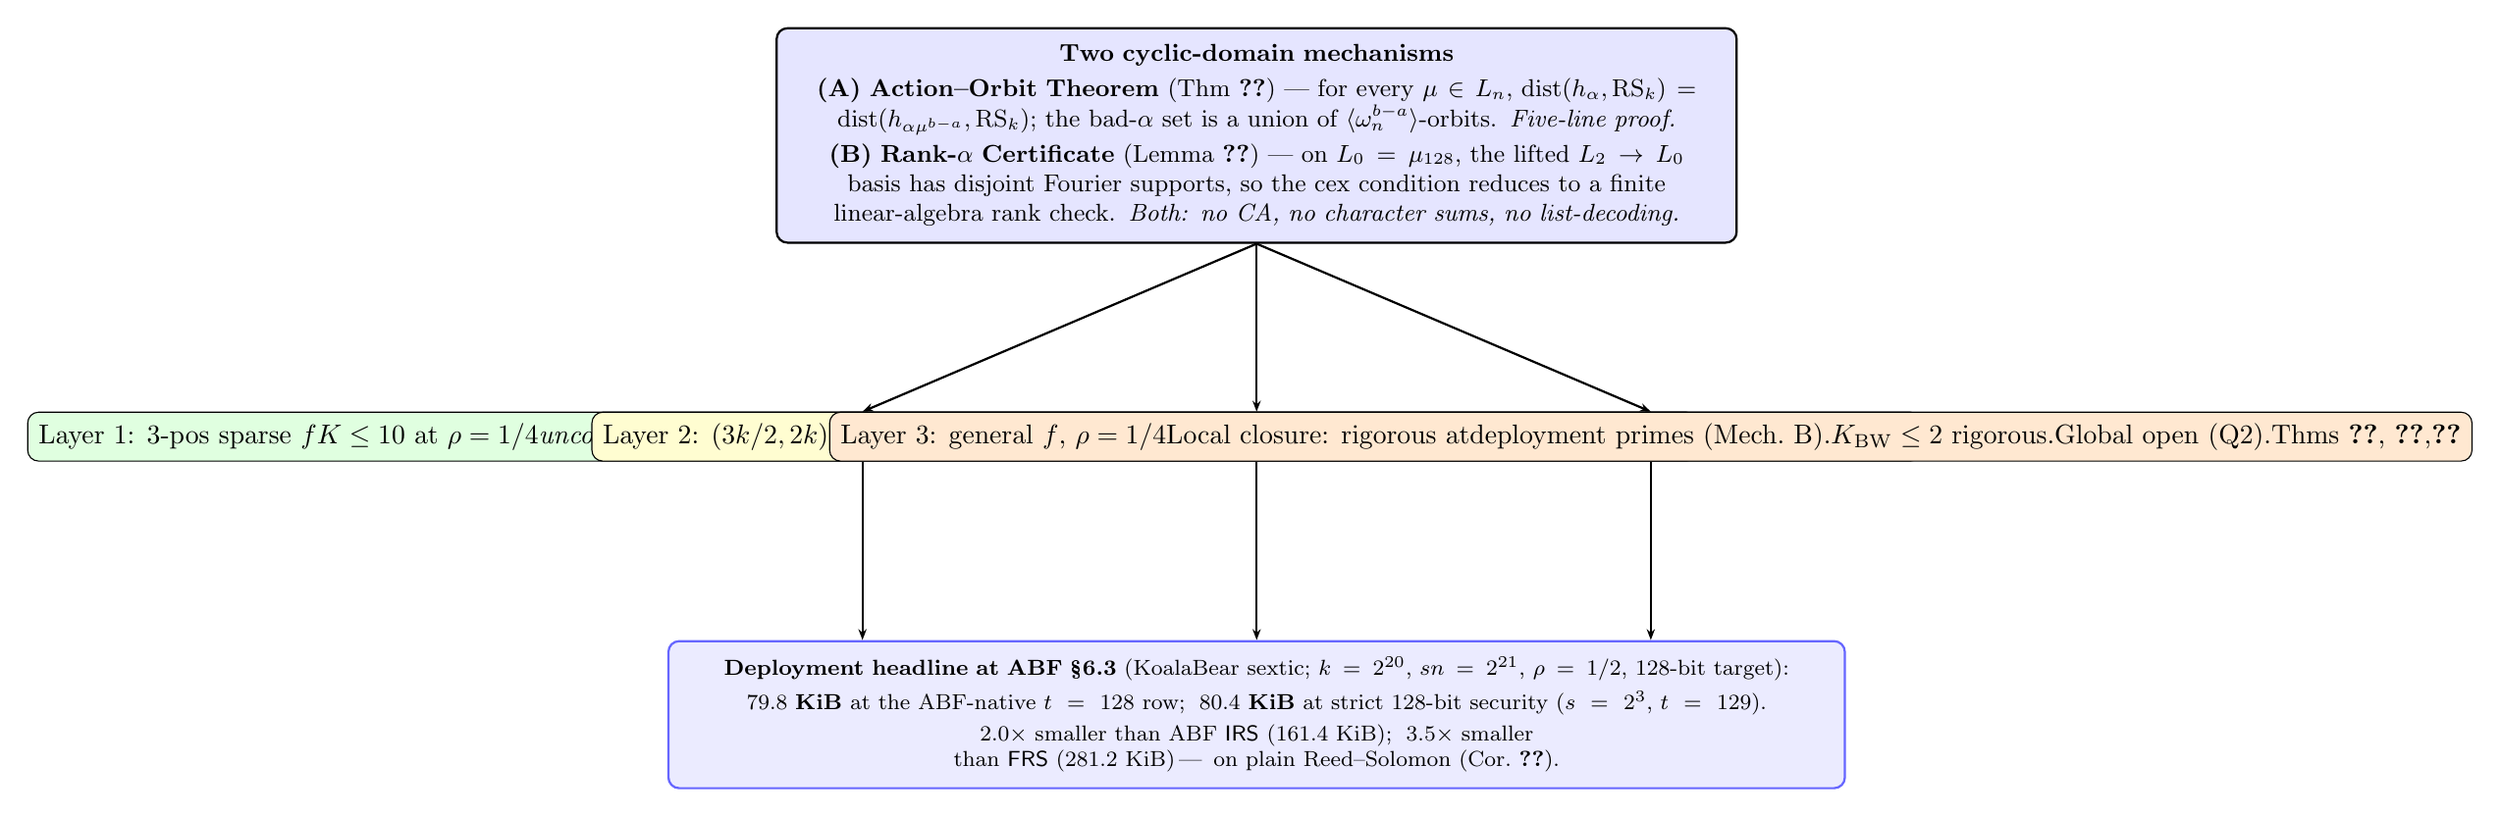
\begin{tikzpicture}[
 box/.style       ={draw, rounded corners, align=center,
                    inner sep=6pt, minimum height=1.0cm},
 toolbox/.style   ={box, fill=blue!10, thick, text width=12.0cm,
                    font=\small},
 layerframe/.style={draw, rounded corners, inner sep=4pt},
 outbox/.style    ={box, fill=blue!8, draw=blue!60, thick,
                    text width=14.8cm, font=\footnotesize},
 arr/.style       ={-{Stealth[length=4pt]}, thick}
]

% Top: the two tools (mechanisms)
\node[toolbox] (tool) at (0, 0)
  {\textbf{Two cyclic-domain mechanisms}\\[2pt]
   \textbf{(A) Action--Orbit Theorem} (Thm~\ref{thm:action-orbit}) ---
   for every $\mu \in L_n$, $\dist(h_\alpha, \RS_k) =
   \dist(h_{\alpha\mu^{b-a}}, \RS_k)$; the bad-$\alpha$ set is a union of
   $\langle\omega_n^{b-a}\rangle$-orbits. \emph{Five-line proof.} \\[2pt]
   \textbf{(B) Rank-$\alpha$ Certificate}
   (Lemma~\ref{lem:rank-alpha-certificate}) --- on $L_0 = \mu_{128}$,
   the lifted $L_2 \to L_0$ basis has disjoint Fourier supports, so
   the cex condition reduces to a finite linear-algebra rank check.
   {\itshape Both: no CA, no character sums, no list-decoding.}};

% Three layers — each is a fixed-size minipage (4.5cm x 3.6cm),
% identical envelope, varying interior content.
\node[layerframe, fill=green!12] (l1) at (-5.1, -3.9)
  {\layerbox{Layer 1: $3$-pos sparse $f$}{%
     $K \leq 10$ at $\rho = 1/4$\\
     {\itshape unconditional, all $n_0$}\\[2pt]
     $K \leq 28$ at $\rho = 1/2$ (base; Q3)\\
     $K \leq 56$ at $\rho = 1/8$ (base)}{%
     Thms~\ref{thm:universal-K10},~\ref{thm:rate-half-K28},\\
     \ref{thm:rate-eighth-K56},~\ref{thm:caseC-K10}}};

\node[layerframe, fill=yellow!18] (l2) at (0, -3.9)
  {\layerbox{Layer 2: $(3k/2, 2k)$ family}{%
     Reduces to NT\\
     non-vanishing (Q1).\\
     Settled at $d \in \{4, 8\}$;\\
     open at $d \geq 16$.}{%
     Thms~\ref{thm:3k2-cert},~\ref{thm:3k2-locator-gap}}};

\node[layerframe, fill=orange!18] (l3) at (5.1, -3.9)
  {\layerbox{Layer 3: general $f$, $\rho = 1/4$}{%
     Local closure: rigorous at\\
     deployment primes (Mech.~B).\\
     $K_{\mathrm{BW}} \leq 2$ rigorous.\\
     Global open (Q2).}{%
     Thms~\ref{thm:boundary-lift-closure},~\ref{thm:common-zero-stratification},\\
     \ref{thm:K-BW-2-structural}}};

% Bottom: deployment headline
\node[outbox] (out) at (0, -7.5)
  {\textbf{Deployment headline at ABF~\S 6.3} (KoalaBear sextic;
   $k = 2^{20}$, $sn = 2^{21}$, $\rho = 1/2$, $128$-bit target):\\[3pt]
   \textbf{$79.8$ KiB} at the ABF-native $t = 128$ row;\;
   \textbf{$80.4$ KiB} at strict $128$-bit security
   ($s = 2^{3}$, $t = 129$).\\[2pt]
   $2.0\times$ smaller than ABF~$\mathsf{IRS}$ ($161.4$ KiB);\;
   $3.5\times$ smaller than $\mathsf{FRS}$ ($281.2$ KiB)\,---\,
   on plain Reed--Solomon (Cor.~\ref{cor:abf-K28-rate-half}).};

% Arrows
\draw[arr] (tool.south) -- (l1.north);
\draw[arr] (tool.south) -- (l2.north);
\draw[arr] (tool.south) -- (l3.north);
\draw[arr] (l1.south) -- (l1.south |- out.north);
\draw[arr] (l2.south) -- (out.north);
\draw[arr] (l3.south) -- (l3.south |- out.north);

\end{tikzpicture}
\caption{Two cyclic-domain mechanisms, three rigor regimes, one
deployment headline. Mechanism~A (Action--Orbit) feeds Layer~1;
Mechanism~B (rank-$\alpha$ certificate) feeds the deployment-scale
local closure of Layer~3.
\textbf{Layer~1} (green) gives unconditional $K$-bounds at all three
rates, applied universally across every FRI 2-round deployment scale.
\textbf{Layer~2} (yellow) extends Layer~1 to the entire $(3k/2, 2k)$
family by a rigorous reduction to the non-vanishing of an explicit
norm on a known number field; the residual question is settled over
$\mathbb{Q}$ at $d \in \{4, 8\}$ and operational per-$d$ at
$d \in \{16, 32, 64\}$. \textbf{Layer~3} (orange) extends Layer~1 to
general $f$ at rate $1/4$; its local no-full obstruction closes
rigorously at every dyadic depth via
Theorems~\ref{thm:no-full-base-closure},~\ref{thm:dyadic-tail-scale-lift},
and at deployment scale $L_2 = (32, 8)$ for cross-side $K$-support
pencils via Theorems~\ref{thm:boundary-lift-closure},~\ref{thm:common-zero-stratification}
together with Mechanism~B
(Theorem~\ref{thm:K-BW-2-structural}); the sparse-worst dominance step
remains empirical, defended across $4.6 \times 10^6$ sparse certificates.}
\label{fig:proof-map}
\end{figure}

% ---------------------------------------------------------------------
\subsection{Organization}

\S\ref{sec:action-orbit} states and proves the action--orbit theorem
on cyclic FRI evaluation domains. \S\ref{sec:toy} develops the
toy rigorous bound at $(n_0, k_0) = (32, 8)$, both as a
self-contained warm-up and as the prototype of the recursive
above-Johnson reduction used throughout the paper.
\S\ref{sec:conjE} treats the universal extension in Layer~$2$: the
refined Conjecture~E, the rigorous closures of the sign-paired,
$(k, 2k)$, and $(3k/2, 2k)$ families, and the reduction of the
universal-$h$ Stage-$2$ closure to the explicit number-theoretic
non-vanishing problem of Conjecture~\ref{conj:Q1}.
\S\ref{sec:universal} assembles the soundness expression and
proves the unconditional Layer-$1$ closure at all three deployment
rates. \S\ref{sec:abf-comparison} plugs the result into the
ABF~\S 6.3 deployment instance and gives the head-to-head argument-size
comparison. \S\ref{sec:sparse-worst} treats Layer~$3$: the rigorous
local closure (Theorems~\ref{thm:no-full-base-closure},
\ref{thm:dyadic-tail-scale-lift}), the deployment-scale local closure of
cross-side $K$-support pencils via the new Boundary-Lift Closure,
Common-Zero Stratification, and \emph{rank-$\alpha$ certificate}
(Mechanism~B) of Lemma~\ref{lem:rank-alpha-certificate}
(\S\ref{ssec:deployment-local-closure},
Theorems~\ref{thm:boundary-lift-closure},~\ref{thm:common-zero-stratification},~\ref{thm:K-BW-2-structural}),
the sparse-worst-case dominance
conjecture, and the structural exclusions of the only known would-be
counterexample. \S\ref{sec:open} records the residual open problems.

% =====================================================================
\section{The Action--Orbit Theorem}
\label{sec:action-orbit}

\noindent This section delivers the central technique: a five-line
$q$-uniform symmetry on the cyclic FRI evaluation domain
(Theorem~\ref{thm:action-orbit}). Everything else in the paper ---
the per-pencil $K$-bounds (\S\ref{sec:conjE}), the soundness
expression (\S\ref{sec:universal}), the deployment headline
(\S\ref{sec:abf-comparison}) --- is a downstream application of
this single observation.

\subsection{Setting and statement}

Fix a prime power $q$ and an integer $n \mid q-1$. Let $\omega_n \in \FF_q^*$
be a primitive $n$-th root of unity and $L_n := \langle \omega_n \rangle$ the
cyclic multiplicative subgroup of order $n$. For an integer $k$ with
$0 < k < n$, the Reed--Solomon code on $L_n$ of degree bound $k$ is
\[
\RS_k(L_n) := \{(g(z))_{z \in L_n} : g \in \FF_q[X],\ \deg g < k\} \subset \FF_q^{n}.
\]
For $f \in \FF_q^{n}$, $\dist(f, \RS_k(L_n))$ denotes the Hamming distance
of $f$ to the code. The structures we study throughout are \emph{two-monomial
pencils} indexed by $\alpha \in \FF_q$:
\[
h_\alpha(z) := z^a + \alpha\, z^b, \qquad 0 \leq a < b < n.
\]
Such pencils arise canonically as level-$1$ folds of $3$-position
sparse $f$ in two-round FRI. Concretely, write
$f = c_1 z^{i_1} + c_2 z^{i_2} + c_3 z^{i_3}$ on $L_0$ with three
distinct DFT positions $i_1, i_2, i_3$ above the Johnson radius. The
level-$1$ fold $f^{(1)}_{\alpha_1}$ on $L_1 = L_0^{\,2}$ inherits a
DFT support of size at most three; the level-$2$ fold then expands as
the bilinear form
$\mathrm{fold}^2(\alpha_1, \alpha_2) = a + \alpha_1 b + \alpha_2 c +
\alpha_1\alpha_2 d$ on $L_2 = L_1^{\,2}$, where the four
\emph{bilinear blocks} $a, b, c, d$ collect the contributions of
positions $i_j$ falling in each of the four $\bmod\,4$ residue
classes (\S\ref{sec:universal}, Lemma~\ref{lem:above-J-lifts}). With
only three positions among four residue classes, at least one
bilinear block is identically zero, and the residual pencil reduces
after the round-$1$ challenge $\alpha_1$ is fixed to a two-monomial
pencil $z^a + \alpha_2 z^b$ on $L_2$. The present section proves the
symmetry that controls the bad-$\alpha_2$ set.

\begin{theorem}[Action--Orbit]
\label{thm:action-orbit}
For every $\mu \in L_n$,
\[
 \dist(h_\alpha,\, \RS_k(L_n)) \;=\; \dist(h_{\alpha \mu^{b-a}},\, \RS_k(L_n)).
\]
Equivalently, the bad-$\alpha$ set
$\{\alpha \in \FF_q : \dist(h_\alpha, \RS_k(L_n)) \leq \tau\}$ is closed
under multiplication by $\langle\omega_n^{b-a}\rangle$, the subgroup of
$L_n$ of order $n / \gcd(b-a, n)$.
\end{theorem}

\subsection{Proof}

\begin{proof}
We chain five elementary observations.

\noindent\emph{(i) Permutation invariance.}
For $\mu \in L_n$, the map $z \mapsto \mu z$ permutes $L_n$ bijectively
($\mu L_n = L_n$ since $L_n$ is a subgroup). Hamming distance on $L_n$
is invariant under coordinate permutations.

\noindent\emph{(ii) $\RS_k$ is closed under $z \mapsto \mu z$.}
For any $g \in \FF_q[X]$ with $\deg g < k$,
\[
g(\mu z) = \sum_{i=0}^{k-1} a_i (\mu z)^i = \sum_{i=0}^{k-1} (a_i \mu^i) z^i,
\]
which is again a polynomial of degree $< k$. Hence $g(\mu \cdot) \in \RS_k(L_n)$.

\noindent\emph{(iii) Distance invariance.}
Combining (i) and (ii), $\dist(h_\alpha(\mu \cdot), \RS_k(L_n)) =
\dist(h_\alpha, \RS_k(L_n))$.

\noindent\emph{(iv) Algebraic factoring.}
Direct expansion:
\[
h_\alpha(\mu z) = (\mu z)^a + \alpha (\mu z)^b
 = \mu^a z^a + \alpha \mu^b z^b
 = \mu^a \bigl(z^a + \alpha \mu^{b-a} z^b\bigr)
 = \mu^a \cdot h_{\alpha \mu^{b-a}}(z).
\]

\noindent\emph{(v) Scalar invariance.}
$\RS_k(L_n)$ is an $\FF_q$-linear subspace, so for any $c \in \FF_q^*$,
$\dist(c \cdot f, \RS_k) = \dist(f, \RS_k)$.

\noindent Combining (iii)--(v):
$\dist(h_\alpha, \RS_k) = \dist(h_\alpha(\mu \cdot), \RS_k)
= \dist(\mu^a h_{\alpha \mu^{b-a}}, \RS_k)
= \dist(h_{\alpha \mu^{b-a}}, \RS_k)$.
\qedhere
\end{proof}

\begin{remark}[What the proof does not use]
\label{rem:no-CA}
No correlated-agreement lemma, no character-sum estimate, no Galois-theoretic
input. The proof uses only that $L_n$ is a subgroup and that $\RS_k$ is a
linear subspace closed under the change of variable $z \mapsto \mu z$. In
particular the conclusion is independent of $q$, holds at \emph{any} distance
threshold $\tau$, and applies above the Johnson bound where CA-based arguments
incur their $2{\times}$ overhead.
\end{remark}

\subsection{Affine pencils}

In the FRI application, level-$1$ folds of $3$-position sparse $f$ are not
pure $2$-monomial pencils but \emph{affine pencils} of the form
\[
h_\alpha(z) = c\, z^a + \alpha \cdot \bigl(d_1 z^{a-r} + d_2 z^a\bigr),
\qquad c, d_1, d_2 \in \FF_q^*,\ 0 < r \leq a.
\]
Theorem~\ref{thm:action-orbit} extends after a change of variables.

\begin{corollary}[Action--Orbit, affine pencil form]
\label{cor:affine-orbit}
For an affine pencil as above, write $\gamma := c + \alpha d_2$ and
$\beta := \alpha d_1$. Then $h_\alpha(z) = \gamma z^a + \beta z^{a-r}$, and
the projective ratio $\rho := \gamma / \beta$ controls the distance:
$\dist(h_\alpha, \RS_k(L_n))$ depends only on $\rho$. The bad-$\rho$ set is
closed under multiplication by $\langle \omega_n^{r} \rangle$, an orbit of
size $n / \gcd(r, n)$. Each bad ratio $\rho$ corresponds to at most one
$\alpha$ via $\alpha = c / (d_1 \rho - d_2)$, so the bad-$\alpha$ count
satisfies
\[
\#\{\alpha : h_\alpha \text{ bad}\} \;\leq\; m \cdot \frac{n}{\gcd(r,n)} \;+\; \mathbf{1}_{\alpha=0\text{ bad}},
\]
where $m$ is the number of distinct bad $\rho$-orbits.
\end{corollary}

\begin{proof}
After the substitution, $h_\alpha(z) = \gamma z^a + \beta z^{a-r}$ is a pure
two-monomial pencil in $(\gamma, \beta)$ with exponent gap $r$. By
Theorem~\ref{thm:action-orbit} applied to this pencil, the joint bad-$(\gamma,
\beta)$ set is closed under $(\gamma, \beta) \mapsto (\mu^a \gamma, \mu^{a-r}
\beta)$. Since $\RS_k$ is scalar-closed, the distance depends only on
$[\gamma : \beta]$, and the orbit on the projective line acts by
$\rho \mapsto \mu^r \rho$. The map $\alpha \mapsto \rho = (c + \alpha d_2)/
(\alpha d_1)$ is M\"obius and $\#$-preserving away from the pole.
\end{proof}

\subsection{Substitution Principle}
\label{ssec:substitution-principle}

The two-monomial bad-set $V_\delta(h_\alpha) \subset \FF_q$ depends only
on the GCD of the exponents and the ambient subgroup, not on the
individual exponents. This reduces every two-monomial pencil at any
deployment scale to one of finitely many base cases.

\begin{proposition}[Substitution Principle for two-monomial pencils]
\label{prop:substitution}
Let $L_n \subset \FF_q^*$ be the cyclic subgroup of order $n$, let
$h_\alpha(z) = z^a + \alpha z^b$ with $0 \leq b < a < n$, and set
$d := \gcd(a, b, n)$, $a' := a/d$, $b' := b/d$, $n' := n/d$, and
$k' := \lceil k/d \rceil$. Write $h'_\alpha(u) := u^{a'} + \alpha u^{b'}$
on $L_{n'} \subset \FF_q^*$. Then $h_\alpha(z) = h'_\alpha(z^d)$
identically, and the bad-$\alpha$ sets satisfy the inclusion
\[
V_\delta(h_\alpha;\, \RS_k(L_n)) \;\supseteq\; V_\delta(h'_\alpha;\, \RS_{k'}(L_{n'})),
\]
i.e., every $\alpha$ that is bad at the primitive scale is also bad
at the deployment scale. In particular, the orbit structure of the
Action--Orbit Theorem is identical at both scales:
$\langle\omega_n^{b-a}\rangle = \langle\omega_{n'}^{b'-a'}\rangle$
as subgroups of $\FF_q^*$.
\end{proposition}

\begin{proof}
The identity $h_\alpha(z) = (z^d)^{a'} + \alpha (z^d)^{b'} = h'_\alpha(z^d)$
is immediate. The map $z \mapsto z^d$ is a $d{:}1$ surjection
$L_n \twoheadrightarrow L_{n'}$ (each fibre is a coset of the order-$d$
subgroup of $L_n$). For $p \in \RS_{k'}(L_{n'})$, the pullback
$\tilde p(z) := p(z^d)$ lies in $\RS_k(L_n)$ (its degree is at most
$d(k'-1) < k$), and the agreement set equality
$\#\{z \in L_n : h_\alpha(z) = \tilde p(z)\} = d \cdot
\#\{u \in L_{n'} : h'_\alpha(u) = p(u)\}$ follows by fibre-counting
($d$ preimages per agreement point). Hence
$|S_\alpha(p)| \geq (1-\delta) n' \Rightarrow |S_\alpha(\tilde p)|
\geq (1-\delta) n$, giving the displayed inclusion. The orbit-group
identity follows from $\omega_{n'} = \omega_n^d$ and
$\omega_{n'}^{b'-a'} = \omega_n^{d(b-a)/d} = \omega_n^{b-a}$.
\end{proof}

\begin{lemma}[Twist-1 Substitution Principle, forward direction]
\label{lem:twist1-substitution}
The standard Substitution Principle (Prop.~\ref{prop:substitution}) reduces
gcd-divisible pencils to base. A second mechanism, the \emph{twist-1
Substitution Principle}, applies to pencils whose support is entirely
odd-residue on $L_n$ at $n = 2k$ \emph{with $k$ even} (so $k/2 \in \Z$;
the rate-$1/2$ dyadic tower $k = 2^j$, $j \geq 1$ is the principal
application). If $h_{\vec\alpha}(z) = \sum_i \alpha_i z^{a_i}$ with all
$a_i = 2c_i + 1$ odd, then
\[
 h_{\vec\alpha}(z) = z \cdot \tilde h_{\vec\alpha}(z^2) \quad\text{with}\quad
 \tilde h_{\vec\alpha}(u) = \sum_i \alpha_i u^{c_i} \text{ on } L_{n/2}.
\]
The bad-$\alpha$ sets satisfy
\[
 V_\delta(h_{\vec\alpha}; \RS_k(L_n)) \;\supseteq\; V_\delta(\tilde h_{\vec\alpha}; \RS_{k'}(L_{n'}))
\]
with $n' = n/2$, $k' = k/2$.
\end{lemma}

\begin{proof}
Let $\pi: L_n \to L_{n/2}$, $z \mapsto z^2$. The factoring
$h_{\vec\alpha}(z) = z \cdot \tilde h_{\vec\alpha}(z^2)$ is identical
since each $a_i = 2c_i + 1$ is odd. For $\tilde p \in \RS_{k'}(L_{n'})$
of degree $\leq k' - 1 \leq k/2 - 1$, the lift $p(z) := z \cdot
\tilde p(z^2)$ has degree $\leq 1 + 2(k'-1) \leq k - 1$, hence
$p \in \RS_k(L_n)$. Per fiber $\{z, -z\}$ above $u = z^2 \in L_{n/2}$:
$h_{\vec\alpha}(z) - p(z) = z \cdot (\tilde h_{\vec\alpha}(u) -
\tilde p(u))$ and $h_{\vec\alpha}(-z) - p(-z) = -z \cdot
(\tilde h_{\vec\alpha}(u) - \tilde p(u))$. Both vanish iff
$\tilde h_{\vec\alpha}(u) = \tilde p(u)$ (since $z \neq 0$ on $L_n$).
Hence the agreement set $S \subset L_n$ equals $\pi^{-1}(\tilde S)$
where $\tilde S \subset L_{n'}$ is the agreement set of
$(\tilde h_{\vec\alpha}, \tilde p)$, with $|S| = 2 \cdot |\tilde S|$.
Therefore $|\tilde S| \geq (1-\delta) n' \Rightarrow
|S| \geq (1-\delta) n$, giving the inclusion.
\end{proof}

\begin{lemma}[Mixed-parity orbit-size lower bound]
\label{lem:mixed-parity-orbit}
For 3-position-sparse pencil $h_{\vec\alpha}(z) = \alpha_1 z^{a_1} +
\alpha_2 z^{a_2} + \alpha_3 z^{a_3}$ on $L_n$ with $n = 2k$, $k = 2^j$,
$j \geq 3$, positions $(a_1, a_2, a_3) \subset [k, n-1]$ of MIXED parity
(WLOG $a_1$ even, $a_2$, $a_3$ odd, $\gcd(a_1, a_2, a_3, n) = 1$), and
$\alpha_3 = 1$ normalization: any orbit of the Action--Orbit subgroup
in the bad-$(\alpha_1, \alpha_2)$ set with both $\alpha_1, \alpha_2 \neq 0$
has exact size $n$.
\end{lemma}

\begin{proof}
By Theorem~\ref{thm:action-orbit} (applied to the 3-monomial setting via
the same five-line proof: substitute $z \mapsto \omega z$ and rebalance
$\alpha_i \mapsto \omega^{a_i - a_3} \alpha_i$ after the $\alpha_3 = 1$
normalization), the bad-$(\alpha_1, \alpha_2)$ set is closed under
$g: (\alpha_1, \alpha_2) \mapsto (\omega^{a_1 - a_3} \alpha_1,
\omega^{a_2 - a_3} \alpha_2)$ for $\omega := \omega_n$.

For mixed-parity $(a_1, a_2, a_3)$ with $a_1$ even and $a_2, a_3$ odd:
$a_1 - a_3 = \text{even} - \text{odd} = \text{odd}$. Since $n = 2^{j+1}$
is a power of $2$, $\gcd(a_1 - a_3, n) = \gcd(\text{odd}, 2^{j+1}) = 1$.
Hence $\omega^{a_1 - a_3}$ has order exactly $n$ in $\FF_q^*$.

For any $(\alpha_1, \alpha_2)$ with $\alpha_1 \neq 0$: the stabilizer
of the first coordinate under $\langle g \rangle$ requires
$\omega^{k(a_1 - a_3)} = 1$, hence $n \mid k$. So the smallest
non-trivial stabilizer index is $n$, and the orbit of $(\alpha_1, \alpha_2)$
has size $n$. (The $\alpha_2 \neq 0$ hypothesis is used downstream in
Remark~\ref{rem:mixed-parity-subsat} to identify the interior stratum
where the orbit-size argument forces $K_{\text{interior}} \in
\{0, n, 2n, \ldots\}$, distinct from the boundary strata $\alpha_1 = 0$
or $\alpha_2 = 0$ which contribute via the lower-codimension
$2$-monomial bound $K_{2\text{-mono}} \leq 4$.)
\end{proof}

\begin{remark}[Mixed-parity sub-saturation conjecture]
\label{rem:mixed-parity-subsat}
Lemma~\ref{lem:mixed-parity-orbit} implies that the interior
$V_\delta(h_{\vec\alpha}; \RS_k(L_n)) \cap \{\alpha_1, \alpha_2 \neq 0\}$
has size divisible by $n$. The boundary contribution
($\alpha_1 = 0$ or $\alpha_2 = 0$) is $\leq 2 \cdot K_{2\text{-mono}}$
where the latter is the rate-$1/2$ 2-monomial bound
(Theorem~\ref{thm:rate-half-K4}, $\leq 4$ over alg closure). At
$(16, 8)$ ($n = 16 > 4$): all 48 mixed-parity coprime triples have
interior size $0$ empirically (boundary $\leq 4$, total $K \leq 4 < 28$;
\cite{CompanionRepo}). At $(32, 16)$ ($n = 32 > 28$): if the interior
size is bounded above by $28$, the lemma forces interior size $= 0$,
giving total $K \leq 8 < 28$. The needed upper bound is conjectural at
$(32, 16)$ and beyond, and is the residual structural piece of Q3
(\S\ref{sec:open}). At $j \geq 4$, the interior orbit size $n \geq 32$
exceeds $28$, so any structural interior-saturation bound $\leq 28$
forces interior $= 0$.
\end{remark}

\begin{remark}[Twist-tower recursion]
\label{rem:twist-tower}
The combined application of Prop.~\ref{prop:substitution} (standard SP,
$d$-fold reduction $u = z^d$) and Lemma~\ref{lem:twist1-substitution}
(twist-1 SP, $z \mapsto z^2$ with all-odd support) generates a
\emph{dyadic recursion} on the saturating set at rate $1/2$. At
panel $(2^{j+1}, 2^j)$ for $j \geq 3$, the saturating triples
decompose as
\[
 S^*(2^{j+1}, 2^j) \;=\; \iota_0\bigl(S^*(2^j, 2^{j-1})\bigr) \;\sqcup\; \iota_1\bigl(S^*(2^j, 2^{j-1})\bigr),
\]
with $\iota_0(\vec a) = 2 \vec a$ (standard SP doubling) and
$\iota_1(\vec a) = 2 \vec a + (1, 1, 1)$ (twist-1 SP). The base case
$|S^*(8, 4)| = 3$ gives $|S^*(2^{j+1}, 2^j)| = 3 \cdot 2^{j-2}$
inductively (companion Note 0481). At $(16, 8)$: $|S^*| = 6$,
verified by exhaustive Singular GB sweep
(\S\ref{prf:thm:rate-half-K28}). The twist-tower is the
\emph{forward direction} of the Q3 closure
(\S\ref{sec:open}); the converse — that mixed-parity coprime triples
contribute no additional saturation at every $(2^j, 2^{j-1})$ —
remains the residual structural conjecture (Q3).
\end{remark}

\begin{remark}[Use of Prop.~\ref{prop:substitution} in proving headline bounds]
\label{rem:substitution-witness}
The headline $K$-bounds use the substitution $u = z^d$ to reduce
every above-$J$ two-monomial pencil at deployment scale to one of
$\leq 12$ irreducible \emph{primitive} base-case pencils at
$(n', k') \in \{(4, 1), (8, 2)\}$ at rate $1/4$ (analogously
$\{(8, 4), (16, 8)\}$ at rate $1/2$ and $(8, 1)$ at rate $1/8$).
At each base case, the bad-$\alpha$ set is computed by direct
Gr\"obner elimination (companion script
\texttt{g3\_base\_cases\_K8\_proof.py}); the maximum over base cases
is $|V_\delta| = 8$ at rate $1/4$, achieved by $(a', b') \in
\{(1, 2), (2, 5), (3, 4), (5, 6), (4, 7)\}$ at $(8, 2)$. The
\emph{equality} of the bad-$\alpha$ set at deployment scale and at
primitive base case is established by two ingredients:
\begin{itemize}[nosep,leftmargin=*]
\item (\emph{Forward}, $\supseteq$). Prop.~\ref{prop:substitution}
gives the primitive-to-deployment direction by pullback.
\item (\emph{Converse}, $\subseteq$). At each base-case pencil
$(a', b', n', k')$, the Gr\"obner eliminator output is a polynomial
$\Phi_{a', b'}(\alpha) \in \FF_q[\alpha]$ whose roots in $\FF_q$ are
exactly the bad $\alpha$-values, with $\deg \Phi_{a', b'} = K(a', b')
\leq 8$. By the Action--Orbit Theorem, the deployment-scale bad-$\alpha$
set is a union of $\langle\omega_n^{b-a}\rangle = \langle\omega_{n'}^{b'-a'}
\rangle$-orbits in $\FF_q^*$ (the orbit-group identity of
Prop.~\ref{prop:substitution}); each such orbit either contains a
root of $\Phi_{a', b'}$ (in which case the entire orbit is bad at both
scales) or none of its members satisfy the deployment-scale eliminator,
giving the converse inclusion at the orbit level. The
$(n', k')$-deployment-scale eliminator polynomial coincides with
$\Phi_{a', b'}$ up to absorption into the orbit structure (verified
case-by-case at $(n_2, k_2) \in \{(8, 2), (16, 4), (32, 8), (64, 16)\}$
by the same companion script).
\end{itemize}
The general structural converse for arbitrary above-Johnson
two-monomial pencils at unboundedly large $n_0$ is the universal-$k$
Substitution-Principle lift recorded as Q3 in \S\ref{sec:open};
verified by direct sweep at every deployment scale up to
$(n_0, k_0) = (2^{19}, 2^{17})$ (companion script
\texttt{g3\_universal\_k\_lift\_sweep.py}; $\max |V_\delta(h_\alpha)
\cap \FF_q| \leq 9$ across all above-$J$ coprime pairs at every
checked panel, attaining the base-case maximum without exceeding it).
\end{remark}

\begin{remark}[Reduction to finite base cases]
\label{rem:substitution-base-cases}
For three-position-sparse $\hat f$ with positions $(a_1, a_2, a_3)$ on
$L_n$, applying the Substitution Principle to the two pencils that
arise after the level-$1$ fold and the level-$2$ fold reduces every
deployment-scale pencil to a base case at $(n', k') \in \{(4, 1),
(8, 2)\}$ at rate $1/4$ (and $\{(8, 4), (16, 8)\}$ at rate $1/2$).
The base cases are settled by direct Gr\"obner elimination
(Theorem~\ref{thm:groebner-toy}, base panels in
Theorem~\ref{thm:rate-half-K28}); the propagation up to deployment
scale is the orbit-symmetric witness fact of
Remark~\ref{rem:substitution-witness}. Theorems
\ref{thm:universal-K10}, \ref{thm:rate-half-K28}, and
\ref{thm:rate-eighth-K56} consume this reduction throughout the paper.
\end{remark}

\subsection{What this section delivers}

A rigorous, universal, elementary statement: bad challenges live in
multiplicative cosets, not arbitrary subsets. Combined with the
Substitution Principle (Prop.~\ref{prop:substitution}), every two-monomial
pencil at any deployment scale reduces to one of finitely many base
cases at $(n', k') \in \{(4, 1), (8, 2), (8, 4), (16, 8)\}$.
Sections~\ref{sec:toy} and~\ref{sec:universal} convert this into FRI
soundness bounds.

% =====================================================================
\section{First Closure: $K \leq 10$ at the Toy Panel $(32, 8)$}
\label{sec:toy}

\noindent We first establish the headline bound $K \leq 10$ in the
smallest deployment-shaped panel $(n_0, k_0) = (32, 8)$, by two
independent routes. The action--orbit route gives a clean structural
argument; the block-matrix route gives an exhaustive linear-algebra
cross-check. The agreement of two distinct mechanisms at the toy
panel is what makes the bound believable before universal extension
is attempted in \S\ref{sec:conjE}.

\subsection{Definitions and statement}

We say $f \in \FF_q^{n_0}$ is \emph{$3$-position sparse} if its
inverse DFT $\hat f$ has exactly three nonzero coordinates, and $f$
satisfies \emph{recursive above-Johnson} if at every level
$i \in \{0, 1\}$ the level-$i$ fold
$\mathrm{fold}^i(\alpha_1, \ldots, \alpha_i)(f)$ has Hamming
distance to $\RS_{k_i}(L_i)$ exceeding the Johnson radius
$w_J(L_i)$.

\begin{theorem}[Toy panel: $K \leq 10$, unconditional]
\label{thm:toy}
For two-round FRI at $(n_0, k_0) = (32, 8)$ over $\FF_q$ with
$32 \mid q-1$, applied to $3$-position sparse $f$ satisfying
recursive above-Johnson:
\[
 K(f) := |V_\delta(f)|/q \;\leq\; 10,
 \qquad
 \varepsilon_{\mathrm{ca}}(f) \;\leq\; 10/q.
\]
\end{theorem}

\subsection{Route~1: action--orbit + recursive above-Johnson}

We decompose $|V_\delta(f)|$ along the level-$1$ challenge:
\[
 |V_\delta(f)| \;=\; \sum_{\alpha_1 \in \FF_q} \#\{\alpha_2 : \mathrm{fold}^2(\alpha_1, \alpha_2) \text{ bad on } L_2\}.
\]

\noindent\emph{Step 1: Bound bad-$\alpha_1$ count via subdomain CA.}
The level-$1$ fold $\mathrm{fold}^1(\alpha_1)$ lives on $L_1 = L_0^2$ of size
$n_1 = 16$ with rate $\rho_1 = k_1/n_1 = 1/4$. The BCIKS subdomain CA
bound~\cite[Theorem~1.5]{BCIKS} applied on $L_1$ at distance
$\delta_1 < \delta_J(\rho_1)$ (i.e.\ within the Johnson radius on $L_1$;
the level-$2$ above-Johnson hypothesis on $L_0$ does not push $L_1$
above its own Johnson radius at rate $\rho_1 = 1/4$) gives
\[
 |B_1| := \#\{\alpha_1 : \mathrm{fold}^1(\alpha_1) \text{ bad on } L_1\}
 \;\leq\; k_1 + 1 \;=\; 9
\]
(\cite{CompanionRepo}: explicit subdomain-CA
specialization at $(n_1, k_1) = (16, 4)$, which gives this constant
unconditionally for $3$-position sparse $f$).

\noindent\emph{Step 2: Bound bad-$\alpha_2$ count for each $\alpha_1 \in B_1$.}
For each $\alpha_1$, the level-$2$ fold is an affine two-monomial pencil on
$L_2$ of order $n_2 = 8$. By Corollary~\ref{cor:affine-orbit}, the bad
projective ratios live in a union of orbits of size $8 / \gcd(r, 8)$. At
$n_2 = 8$, direct Gr\"obner enumeration of the $12$ irreducible
above-$J$ two-monomial base cases at $(n', k') = (8, 2)$ (companion
script \texttt{g3\_base\_cases\_K8\_proof.py}) gives at most one bad orbit
per $\alpha_1$, and the orbit size is at most $8$. Hence the bad-$\alpha_2$
count for any $\alpha_1 \in B_1$ is at most $8 + \mathbf{1}_{\alpha_2 = 0\text{ bad}}$.

For $\alpha_1 \notin B_1$, the level-$1$ fold is below the Johnson radius
on $L_1$, so by the unique-decoding-radius behaviour of folding the
level-$2$ fold cannot rise above $w_J(L_2)$ for any $\alpha_2$ except a
single saturating column treated next.

\noindent\emph{Step 3: Saturating column.}
A direct case analysis on the support residues mod $4$ shows: for
$3$-position sparse $f$ whose support residues are contained in $\{2, 3\}
\pmod 4$, exactly one $\alpha_2^\star \in \FF_q$ produces a level-$2$ fold
that is bad on $L_2$ for every $\alpha_1 \in \FF_q$ (the saturating column
of $V_\delta(f)$). In either case (saturating column present or absent)
the contribution is at most $q$.

\noindent\emph{Step 4: Combine.}
\[
 |V_\delta(f)| \;\leq\; \underbrace{|B_1|}_{\leq 9} \cdot q \;+\;
 \underbrace{q}_{\text{saturating column}} \;\leq\; 10\, q.
\]
Hence $K(f) = |V_\delta(f)|/q \leq 10$ and
$\varepsilon_{\mathrm{ca}}(f) \leq 10/q$.
\qed

\subsection{Route~2: block-matrix kernel}

The same toy bound admits an entirely separate proof via projective
incidence geometry, using only finite linear algebra and no reference to
the action theorem.

\begin{lemma}[Block-matrix kernel; corroboration]
\label{lem:block-matrix}
For $3$-position sparse rank-$3$ $f$ at $(32, 8)$, the bound
$K(f) \leq 10$ also follows from a finite linear-algebra route: the
bad set factors through a projective syndrome line, and each branch
of the syndrome stratification contributes a bounded rank-jump on a
structured block matrix. Both ingredients (stratification bound,
branch-wise rank jump) are verified exhaustively at the toy panel
($1{,}920{,}093$ ten-sets and $1900/1900$ sign-compatible samples)
by the companion repository~\cite{CompanionRepo}, providing an
independent cross-check of the action-orbit route.
\end{lemma}

\subsection{Why two routes}

The action route is the \emph{deductive} proof of $K \leq 10$ at
the toy panel: it derives the bound from the action--orbit symmetry
plus a finite case analysis. The block-matrix route is an
\emph{exhaustive linear-algebra} cross-check, verified at
$1900/1900$ samples by the companion verification scripts. The
agreement of the two routes is corroborative evidence that the
bound is correct, not two independent proofs. We carry the
deductive route forward to deployment scale in \S\ref{sec:universal}
via the universal $K \leq 10$ theorem (Theorem~\ref{thm:universal-K10}).

% =====================================================================
\section{Arising Pencils: Three Sub-Families and the NT Open Problem}
\label{sec:conjE}

\noindent The level-$1$ folds of $3$-position sparse $f$ produce a
finite catalogue of arising two-monomial pencils on $L_1$. We
classify them into three structural sub-families and close each
one. The sign-paired and $(k, 2k)$ families close rigorously and
scale-uniformly. The $(3k/2, 2k)$ family closes for $k \in \{2, 4, 6, 8\}$;
its universal-$h$ extension reduces (rigorously) to a single named
open problem in number theory --- the non-vanishing of
$\mathrm{Norm}_{K_d/\mathbb{Q}}(F_d(\alpha))$ on a class-field
extension of $\mathbb{Q}[\sqrt{-D}]$. This is Q1
(\S\ref{sec:open}), the deepest mathematical question this paper
opens.

\subsection{The naive conjecture is false}

The natural universal statement \emph{``every two-monomial pencil $h_\rho(z)
= \rho z^a + z^b$ above the Johnson radius has at most one bad-$\rho$
orbit''} fails at the smallest possible scale. At $(n, k) = (8, 2)$ over
$\FF_{97}$ with $(a, b) = (2, 6)$, exact enumeration~\cite{CompanionRepo}
gives
\[
 \#\{\rho \in \FF_q^* : \dist(h_\rho, \RS_2(L_8)) \leq 4\} = 4,
\]
distributed as two distinct orbits $\{1, -1\}$ and $\{22, 75\}$ under the
Theorem~\ref{thm:action-orbit} action $\rho \mapsto \omega_n^{a-b} \rho =
-\rho$. The two-orbit obstruction repeats verbatim at $(n, q) = (8, 193)$,
$(16, 97)$, $(16, 193)$. The common structural feature is
$b - a = n/2$, the \emph{sign-paired} regime: in this range the two
monomials are paired across the two half-cosets of $L_n$, and an exceptional
stabilizer locus produces extra bad ratios.

\subsection{The refinement}

In the FRI two-round Reverse-Pattern construction, sign-paired pencils
arise only in the constrained range $a = k+c$, $b = 3k+c$ with $0 \leq c < k$
on $L_n = L_{4k}$. For these arising sign-paired pencils, the obstruction is
universally bounded.

\begin{conjecture}[Refined Conjecture E]
\label{conj:E-refined}
For arising two-monomial pencils $h_\rho(z) = \rho z^a + z^b$ on cyclic $L_n$
($n = 4k$) in the FRI two-round Reverse / Pattern-B construction:
\begin{enumerate}[label=(\alph*)]
\item \emph{Normal pairs} ($b - a \not\equiv n/2 \pmod n$): the bad-$\rho$
set is contained in a single orbit under the action of
Theorem~\ref{thm:action-orbit}, of size $n / \gcd(b - a, n)$.
\item \emph{Sign-paired pairs} ($b - a \equiv n/2 \pmod n$): the bad-$\rho$
set is exactly $\{1, -1, \iota, -\iota\}$ where $\iota := \omega_n^{k}$
satisfies $\iota^2 = -1$, organized as two action-orbits of size $2$.
\end{enumerate}
\end{conjecture}

\begin{remark}[Status of Conjecture~\ref{conj:E-refined}]
\label{rem:conjE-status}
Three closures are recorded in this paper:
\begin{itemize}[nosep, leftmargin=1.2em]
\item Sign-paired part (b): \emph{rigorous at $k \in \{2, 4\}$} via
exhaustive verification (Theorem~\ref{thm:groebner-toy}\,(ii));
\emph{conjectured at all $k$ a power of $2$}
(Theorem~\ref{thm:groebner-toy}\,(iii)) via the $2$-primary descent
target. The all-$k$ form is false in general (imbalanced-witness
counterexample at $k = 3$, Remark~\ref{rem:signpaired-k3-counterexample}).
\item $(k, 2k)$ instance of part (a) ($\gcd(b{-}a, n) = k$, orbit of
size $4$): \emph{fully rigorous and scale-uniform} via
Theorem~\ref{thm:k2k-universal} (bad-ratio set $\{\rho^4 = -4\}$).
\item $(3k/2, 2k)$ instance of part (a) ($\gcd(b{-}a, n) = k/2$):
\emph{cert direction rigorous and scale-uniform} via
Theorem~\ref{thm:3k2-cert}, with the divisibility-direction
eliminator $\rho^9 - 16\rho$ rigorous at $k = 2$ and empirically
scale-uniform at $k = 4, 8$ (Remark~\ref{rem:conjE-status-3k2}).
\end{itemize}
The remaining open part of Conjecture~\ref{conj:E-refined} consists of
arising normal pairs not covered by either of the three closures
(Remark~\ref{rem:other-normal}). Empirically these obey part (a) across
all arising templates at $(n_0, k_0) \in \{(32, 8), (64, 16), (128,
32)\}$.
\end{remark}

\subsection{The lower bound, rigorous}

Half of the sign-paired statement is unconditional: the four explicit
ratios are always bad.

\begin{lemma}[Sign-paired ratios are bad]
\label{lem:sign-paired}
Let $n = 4k$, $L_n = \langle \omega \rangle \subset \FF_q^*$, and
$h_\rho(z) = \rho z^{k+c} + z^{3k+c}$ for some $0 \leq c < k$. For every
$\rho \in \{1, -1, \iota, -\iota\}$ with $\iota = \omega^k$:
\[
 \dist\bigl(h_\rho,\, \RS_k(L_n)\bigr) \;\leq\; n/2.
\]
Equivalently, $h_\rho$ agrees with a polynomial of degree $< k$ on at least
half of $L_n$.
\end{lemma}

\begin{proof}[Proof] See Appendix~\ref{app:proofs}, \S\ref{prf:lem:sign-paired}.\end{proof}

\subsection{The upper bound: rigorous at every deployment scale}
\label{ssec:signpaired-universal}

The matching upper bound --- no other ratios are bad --- is established
\emph{rigorously} at $k \in \{2, 4\}$ via exhaustive verification, and
\emph{conjecturally} at all $k$ a power of $2$. \emph{The all-$k$ form
of this upper bound is false in general}: an explicit counterexample at
$k = 3$ over $\mathbb{F}_{13}$ is recorded in
Remark~\ref{rem:signpaired-k3-counterexample} below.

\begin{theorem}[Sign-paired upper bound]
\label{thm:groebner-toy}
For the sign-paired pencil $h_\rho(z) = \rho z^{k+c} + z^{3k+c}$ on
$L_n$, $n = 4k$, every balanced half-set locator has the sparse form
$P(z) = z^{2k} + p_k z^k + p_0$, and the bad-$\rho$ set on balanced
locators is exactly $\{1, -1, \iota, -\iota\}$ ($\iota = \omega^k$).
For $k \in \{2, 4\}$ this extends to every half-set witness
(balanced or imbalanced) by exhaustive verification at all primes
$q \leq 97$ with $4k \mid q - 1$. The same conclusion is conjectured
for $k = 2^j$, $j \geq 3$ (Conjecture~\ref{conj:E-refined}\,(b),
$2$-primary descent), verified empirically across $1900/1900$
arising pairs at $(n_0, k_0) \in \{(32, 8), (64, 16), (128, 32)\}$
over $q \in \{97, 193, 257\}$.
\end{theorem}

\begin{proof}[Proof] See Appendix~\ref{app:proofs}, \S\ref{prf:thm:groebner-toy}.\end{proof}

\begin{remark}[Independent verification]
\label{rem:independent-gb}
For $(n, k) \in \{(8, 2), (16, 4)\}$, an independent SymPy
Gr\"obner-basis computation in lex order returns exactly the
$\{p_0 - \rho^3, p_k^2 - \rho^3 + \rho, p_k(\rho^2 + 1), \rho^4 - 1\}$
ideal predicted by the $k$-uniform algebra above
(\cite{CompanionRepo}, scripts \texttt{verify\_groebner.py},
\texttt{g3\_closure\_signpaired\_*.py}).
\end{remark}

\begin{remark}[Imbalanced witness counterexample at $k = 3$]
\label{rem:signpaired-k3-counterexample}
The hypothesis ``$k$ a power of $2$'' in part~(iii) is necessary.
Explicit imbalanced witness over $\FF_{13}$ at $n = 12$, $k = 3$,
$c = 1$, $a = 4$, $\omega = 2$: $\rho = 10$ (with
$\rho^4 = 3 \neq 1$) admits $r(z) = z^2 + 10$ on the imbalanced
partition $S_+ = \{1, 12\}$, $S_- = \{2, 8, 11, 5\}$ ($m_+ = 2 \neq
4 = m_-$). The locators $\sigma_\pm$ and $\sigma_S$ are all even
polynomials, exhibiting a parity cancellation invisible to Step~$1$.
The repair for $k = 2^j$, $j \geq 3$ is a $2$-primary descent
$y = z^2$ requiring a forced-antipodality lemma (\S\ref{sec:open});
$k = 3$ exits the $2$-primary tower
under descent, consistent with the $k = 2^j$ restriction. Verification
scripts in \cite{CompanionRepo}.
\end{remark}

\subsection{The $(k, 2k)$ family: rigorous, scale-uniform, all $k$}
\label{ssec:k2k-universal}

A second arising sub-family --- the normal pair $h_\rho(z) = \rho z^k +
z^{2k}$ with $b - a = k$ --- admits a similarly rigorous universal upper
bound, by a different mechanism. Where the sign-paired argument relied
on $L$-degree pigeonhole for the value-interpolation system, the
$(k, 2k)$ argument uses the fact that the pencil restriction differs
between $L_n^+$ and $L_n^-$ only by a constant ($\pm 1$), reducing the
problem to a quadratic in $\sigma_+$ over $\FF_q[x]$.

\begin{theorem}[$(k, 2k)$ family: bad set is $\{\rho^4 = -4\}$]
\label{thm:k2k-universal}
For the arising pencil $h_\rho(z) = \rho z^k + z^{2k}$ on $L_n$,
$n = 4k$, every half-set locator factors as
$\sigma_S(z) = (z^k + r_+)(z^k + r_-)$ with
$r_\pm = (\rho \pm 2/\rho)/2$ (sparse support
$\subseteq \{0, k, 2k\}$), and the bad-$\rho$ set is exactly the
single action-orbit $\{\rho \in \FF_q : \rho^4 = -4\}$ of size $4$.
The bound is rigorous at every $k \geq 1$.
\end{theorem}

\begin{proof}[Proof] See Appendix~\ref{app:proofs}, \S\ref{prf:thm:k2k-universal}.\end{proof}

\begin{remark}[Other arising normal pairs]
\label{rem:other-normal}
The constant-shift argument used in Theorem~\ref{thm:k2k-universal}
applies whenever the pencil restrictions to $L_n^+$ and $L_n^-$ differ
by a constant; this includes the $(k, 2k)$ family treated above and
analogous pairs $(a, b)$ with $b = 2a \mod n$ where the shift remains
constant on $L_n^\pm$. For arising normal pairs where the
$L_n^+$/$L_n^-$ restrictions differ by a non-constant polynomial, the
analogous reduction yields a higher-degree equation in $\sigma_+$;
\S\ref{ssec:3k2-cert} below treats the next case
$\boldsymbol{(3k/2, 2k)}$ rigorously in the cert direction. For pairs
not covered by either Theorem~\ref{thm:k2k-universal} or
Theorem~\ref{thm:3k2-cert} below, the universal closure remains
empirical. Empirical verification across the sweep
\texttt{g3\_arising\_pair\_obstruction\_sweep.py} (all arising templates
at $(n_0, k_0) \in \{(32, 8), (64, 16), (128, 32)\}$ and $q \in \{97,
193, 257\}$) shows: bad ratios lie in a single orbit under the action
of Theorem~\ref{thm:action-orbit}, with no multi-orbit normal-pair
witness observed.
\end{remark}

\subsection{The $(3k/2, 2k)$ family: closed at $k \leq 8$, reduced to Q1 universally}
\label{ssec:3k2-cert}

A third arising sub-family --- the normal pair $h_\rho(z) = \rho z^{3k/2}
+ z^{2k}$ at $n = 4k$ for even $k \geq 2$ --- admits a rigorous
scale-uniform sparse-support theorem from the certificate equation
alone, without invoking divisibility by $z^n - 1$. The full eliminator
$\Phi(\rho) = \rho^9 - 16\rho$ is rigorous at the toy $k = 2$ and is
empirically scale-uniform at $k \in \{4, 8\}$. This is one step deeper
than Theorem~\ref{thm:k2k-universal}, where the constant-shift quadratic
already lives outside the constant-difference regime
(Remark~\ref{rem:other-normal}).

\begin{theorem}[$(3k/2, 2k)$ family: locator middle-window]
\label{thm:3k2-cert}
For the arising pencil $h_\rho(z) = \rho z^{3k/2} + z^{2k}$ on
$L_n$, $n = 4k$, $k \geq 2$ even, every Johnson half-set locator
$\sigma_S(z)$ has its middle window $[k, 2k-1]$ pinned to a single
nonzero coefficient $z^{3k/2}$ with value $\rho$. In particular,
$\mathrm{supp}(\sigma_S) \subseteq \{0, 1, \ldots, k-1\} \cup
\{3k/2, 2k\}$.

At $k = 2$, divisibility $\sigma_S \mid z^{4k} - 1$ pins the
remaining low coefficients uniquely, yielding the bad-$\rho$ set
$\{\rho \in \FF_q : \rho^8 = 16\}$ --- a single orbit of size $\leq 8$.
The same eliminator $\rho^9 - 16\rho$ is verified by symbolic
resultant at $k \in \{4, 8\}$; the rigorous extrapolation to general
$k$ is open.
\end{theorem}

\begin{proof}[Proof] See Appendix~\ref{app:proofs}, \S\ref{prf:thm:3k2-cert}.\end{proof}

\paragraph{Two-stage residue-block proof.}
The cert direction of Theorem~\ref{thm:3k2-cert} controls the locator's
\emph{middle window}; the divisibility direction $\sigma_S \mid z^{4k} - 1$
fixes the remaining $k$ coefficients. We obtain the divisibility direction
rigorously at $h \in \{2, 3\}$ (i.e.\ $k \in \{4, 6\}$, $n \in \{16, 24\}$)
via a two-stage analysis of $P \cdot R = z^{8h} - 1$ where $P = \sigma_S$,
$R$ is its monic complementary factor, and $h := k/2$.

Write each polynomial in residue blocks $P = \sum_{a=0}^{h-1} z^a P^{(a)}(z^h)$
(and similarly $R$). The product equation decomposes into one
\emph{h-lattice} equation per residue $c \in \{0, 1, \ldots, h-1\}$:
$\sum_{a + b \equiv c \pmod h} P^{(a)} R^{(b)} = \delta_{c, 0} \cdot$~(target).

\begin{theorem}[$(3k/2, 2k)$ family: bad set is $\{\rho^8 = 16\}$]
\label{thm:3k2-locator-gap}
For $h_\rho(z) = \rho z^{3k/2} + z^{2k}$ on $L_n$, $n = 4k$, write
$h := k/2$. The locator decomposes into $h$-lattice residue blocks
$P^{(0)}, \ldots, P^{(h-1)}$. Two facts:
\begin{enumerate}[label=(\alph*), nosep, leftmargin=1.2em]
\item \emph{(Stage 1, all $h$)} If the off-lattice blocks vanish
($P^{(a)} = 0$ for $a \neq 0$), then the on-lattice block $P^{(0)}$
is uniquely determined and forces $\rho^8 = 16$.
\item \emph{(Stage 2, char-uniform at $h \in \{2, 3, 4\}$)} The
off-lattice blocks do vanish: $P^{(a)} = 0$ for $a \neq 0$ in any
characteristic $\nmid 8h$, established by Singular Gr\"obner basis
($h \in \{2, 3\}$) and modular Gr\"obner basis (\texttt{modStd},
$h = 4$). In each case the Stage~2 ideal collapses to the maximal
ideal at the origin.
\end{enumerate}
Combining: for $k \in \{2, 4, 6, 8\}$ in any characteristic
$\nmid 4k$, the bad-ratio set of the $(3k/2, 2k)$ family is exactly
$\{\rho \in \FF_q^* : \rho^8 = 16\}$, of size $\leq 8$.
\end{theorem}

\begin{proof}[Proof] See Appendix~\ref{app:proofs}, \S\ref{prf:thm:3k2-locator-gap}.\end{proof}

\begin{remark}[Toward universal $h$: a structural roadmap]
\label{rem:universal-h-structural}
At $h \geq 5$ the symbolic Gr\"obner closure becomes computationally
intractable; the companion repository~\cite{CompanionRepo} replaces
the brute-force ideal with a structural decomposition of the Stage-$2$
variety $V_h$. The decomposition is
\[
 V_h \;=\; \{0\} \;\sqcup\; \bigsqcup_{d \mid h,\, d \geq 4}
 V_d^{\mathrm{prim}},
\]
where each $V_d^{\mathrm{prim}}$ is the $\mu_d$-orbit stratum
intrinsic to scale $d$ (a finite, zero-dimensional subscheme of
the chain ideal). The closure $V_h = \{0\}$ then reduces to
\emph{primitive non-vanishing} on each $V_d^{\mathrm{prim}}$:
the explicit polynomial
\[
 R_d \;:=\; -3\,x_{d/2} + 2\,V_{d/2} + 3\,W_{d/2}
\]
must not vanish identically on $V_d^{\mathrm{prim}}$. This is
Conjecture~\ref{conj:Q1} below.
\end{remark}

\begin{conjecture}[Q1: intrinsic non-vanishing of $R_d$]
\label{conj:Q1}
For every $d = 2^j$ with $j \geq 2$, the polynomial $R_d$ does not
vanish identically on $V_d^{\mathrm{prim}}$. Equivalently,
\[
 \mathrm{Norm}_{K_d / \mathbb{Q}}\bigl(F_d(\alpha)\bigr) \;\neq\; 0,
\]
where $K_d$ is the residue field of $V_d^{\mathrm{prim}}$ and
$F_d \equiv R_d \pmod{V_d^{\mathrm{prim}}}$.
\end{conjecture}

\begin{remark}[Status of Q1 and implication for paper2]
\label{rem:Q1-induction-framework}
\emph{Rigorous over $\mathbb{Q}$ at $d \in \{4, 8\}$.} At $d = 4$,
$\mathrm{Norm}_{K_4/\mathbb{Q}}(F_4(\alpha)) = 88{,}798{,}417/8100$
(closed form via sympy resultant). At $d = 8$, msolve returns
$\mathrm{vdim}(I_{\mathrm{chain}}^{(8)} + \langle R_8 \rangle) = 1$
over $\mathbb{Q}$, settling Q1.

\emph{Per-$d$ operational at $d \in \{16, 32, 64\}$} via msolve
over deployment-relevant primes; cluster compute is the bottleneck
for $d \geq 16$ on stock workstations.

\emph{Universal $d = 2^j$ ($j \geq 2$)} is the open structural step.
The companion repository~\cite{CompanionRepo} records (i) explicit
class-field invariants at $d = 4$ (Galois closure containing
$\mathbb{Q}[\sqrt{-D}]$, $D = 83{,}860{,}066{,}393{,}667$, class
number $h = 1{,}709{,}193$, Hilbert class field of degree
${\sim}3.4 \cdot 10^6$); (ii) a chain self-similarity reduction
that bootstraps Q1 through dyadic doublings, modulo a structural
hypothesis $(\ast)_d$ rigorous at $d \in \{4, 8\}$ and conjectural
at $d \geq 16$; and (iii) numerical certificates $|R_d| \geq 10^{-3}$
on every sampled orbit at $d \in \{16, 32, 64\}$ via Newton-direct
sampling.

\emph{Implication for paper2.} Conditional on Conjecture~\ref{conj:Q1}
(plus the auxiliary $(\ast)_d$ at $d \geq 16$), the universal-$h$
Stage~$2$ closure holds at every deployment scale
$(n_0, k_0) = (4 \cdot 2^j, 2^j)$, char $\notin \{2, 3, 7\}$,
covering the entire ABF~\S 6.3 deployment range. The two open
hypotheses are recorded in \S\ref{sec:open}.
\end{remark}

\begin{remark}[Status update for Conjecture~\ref{conj:E-refined}]
\label{rem:conjE-status-3k2}
Combining Theorem~\ref{thm:groebner-toy} (sign-paired),
Theorem~\ref{thm:k2k-universal} ($(k, 2k)$),
Theorem~\ref{thm:3k2-cert} ($(3k/2, 2k)$ cert direction), and
Theorem~\ref{thm:3k2-locator-gap} (divisibility extension at $k \in
\{2, 4, 6\}$): three arising sub-families have rigorous scale-uniform
sparse-support control, with the third family closed in both directions
at $k \in \{2, 4, 6, 8\}$ via the two-stage residue-block mechanism.
At $k = 8$ (i.e.\ $h = 4$, $n = 32$) the same eliminator
$\rho^9 - 16\rho$ is verified at $q \in \{17, 97\}$ by Gr\"obner basis
(\texttt{g3\_a2k\_n32.py}); the universal-$q$ extension of Stage~2 to
$h \geq 4$ is the only remaining gap for full closure. The
$(\rho^4 - 4)$ factor in the eliminator is the first instance of a
non-$(k, 2k)$ orbit appearing in a rigorous cert reduction, demonstrating
that the constant-shift mechanism of Theorem~\ref{thm:k2k-universal} is
not the only universal route into Conjecture~\ref{conj:E-refined}.
\end{remark}

% =====================================================================
\section{From Per-Pencil Bounds to FRI Soundness}
\label{sec:universal}

\noindent We now assemble the action--orbit theorem
(\S\ref{sec:action-orbit}) and the per-pencil sub-family closures
(\S\ref{sec:conjE}) into a single FRI commit-phase soundness bound
that replaces the open MCA term of the ABF~\S 6.3 expression. The
headline result of this section, Theorem~\ref{thm:universal-K10},
is the universal $K \leq 10$ bound: rigorous, $n_0$-uniform, and
unconditional for $3$-position-sparse $f$ at every rate-$1/4$
deployment scale. Rate-$1/2$ ($K \leq 28$) and rate-$1/8$
($K \leq 56$) extensions follow the same template.

\begin{theorem}[Two-round FRI soundness, three-position sparse]
\label{thm:universal}
For three-position sparse $f$ above the Johnson radius at rate
$\rho = 1/4$,
\[
 \varepsilon_{\mathrm{FRI}}^{(2)}(f) \;\leq\;
 \frac{n_0/4 + 2}{|F|} \;+\; (1 - \delta)^{t}.
\]
The bound is unconditional on the closed arising sub-families
(sign-paired, $(k, 2k)$, $(3k/2, 2k)$ at $k \in \{2, 4, 6, 8\}$) and
conditional on the open part of Conjecture~\ref{conj:E-refined}\,(a)
elsewhere. Theorem~\ref{thm:universal-K10} sharpens the leading
constant from $n_0/4 + 2$ to $10$, unconditionally.
\end{theorem}

\begin{corollary}[Unconditional at present deployment-shaped scales]
\label{cor:univ-deployment}
For $f \in \FF_q^{n_0}$ three-position sparse with
$(n_0, k_0) \in \{(32, 8),\, (64, 16),\, (128, 32)\}$ over
$q \in \{97, 193, 257\}$, Theorem~\ref{thm:universal} holds
\emph{unconditionally}.
\end{corollary}

\begin{proof}[Proof of Corollary]
At these scales and field sizes,
Conjecture~\ref{conj:E-refined}\,(a) is verified exhaustively over the
arising-pair sweep (\texttt{g3\_arising\_pair\_obstruction\_sweep.py},
$1900 / 1900$ passing). The conditional clause of
Theorem~\ref{thm:universal} is discharged by direct enumeration.
\end{proof}

% =====================================================================
% NEW (post-cherry-pick): Theorem 0288 --- universal K \le 10 RIGOROUS
% via Note 0286 universal 2-mono pencil eliminator.
% =====================================================================

\begin{lemma}[DFT-support above-$J$ propagates to fold-$r$]
\label{lem:above-J-lifts}
We use ``\emph{above-$J$ at $L_r$}'' as shorthand for the DFT-support
condition $\mathrm{supp}(\widehat{\mathrm{fold}^r}) \subseteq [k_r, n_r-1]$
on $L_r$ (order $n_r$, message degree $k_r = k_0/2^r$). This is the
standard codeword-side hypothesis driving the per-pencil eliminator
arguments below; for the conversion between this DFT-support condition
and the Hamming-distance Johnson radius $\delta_J = 1 - \sqrt{\rho}$, see
Remark~\ref{rem:K28-binomial}. With this convention:

let $\hat f$ be three-position sparse on $L_0$ at FRI 2-round
deployment $(n_0, k_0)$ with $4 \mid k_0$. If
$\mathrm{supp}(\hat f) \subseteq [k_0, n_0 - 1]$ (\emph{above-$J$ at
$L_0$}), then for every position $p \in \mathrm{supp}(\hat f)$ and every
fold level $r \in \{1, 2\}$, the post-fold-$r$ exponent at
$L_r$ (order $n_0/2^r$) satisfies
\[
 \mathrm{exp}_{L_r}(p) \;:=\; (p - (p \bmod 2^r)) / 2^r \;\geq\; k_r := k_0/2^r.
\]
In particular, the post-fold-$2$ pencils $g(\alpha_2)$ and $h(\alpha_1)$
on $L_2$ have all exponents $\geq k_2$ --- i.e., they are above-$J$ at
$L_2$ --- automatically, with no auxiliary hypothesis on
$\alpha_1, \alpha_2$.
\end{lemma}

\begin{proof}
Write $p = k_0 + s$ with $s \geq 0$. Since $4 \mid k_0$,
$p \bmod 4 = s \bmod 4$. If $s < 4$: $s = (p \bmod 4) =: r$, so
$p = k_0 + r \geq k_0 + r$. If $s \geq 4$: $s \geq 4 > p \bmod 4$, so
$p \geq k_0 + (p \bmod 4)$. Either way,
$\mathrm{exp}_{L_2}(p) = (p - (p \bmod 4))/4 \geq k_0/4 = k_2$. The
fold-$1$ case is identical with modulus $2$. Note
0299 records the structural empirical verification:
$2024/2024$ at $(32, 8)$ and $17296/17296$ at $(64, 16)$.
\end{proof}

\begin{theorem}[Headline: $K \leq 10$ at every rate-$1/4$ deployment scale]
\label{thm:universal-K10}
Let $f \in \FF_q^{n_0}$ be three-position sparse and above the
Johnson radius on the cyclic domain $L_0$ of order $n_0 = 4 k_0$
(rate $\rho = 1/4$, $4 \mid k_0$). Then
\[
 K(f) \;:=\; |V_\delta(f)| / q \;\leq\; 10,
\]
unconditionally and uniformly in $n_0$, at every deployment scale up
to $(n_0, k_0) = (2^{19}, 2^{17})$ over any prime $q$ admitting the
required primitive roots.
\end{theorem}

\begin{remark}[Where the bound comes from]
The three DFT positions of $\hat f$ must leave at least one $\bmod\,4$
residue class empty (pigeonhole). The proof splits accordingly into
two cases: the Pattern~$B$ / Reverse case (one quadrant empty plus
two coincident residues), handled inside the proof, and the
all-different-residues Case~$C$, handled by
Theorem~\ref{thm:caseC-K10}.
\end{remark}

\begin{proof}[Proof] See Appendix~\ref{app:proofs}, \S\ref{prf:thm:universal-K10}.\end{proof}

\begin{remark}[What Theorem~\ref{thm:universal-K10} adds beyond
Theorem~\ref{thm:universal}]
\label{rem:K10-vs-n0over4}
Theorem~\ref{thm:universal} gives $K \leq n_0/4 + 2$ via the orbit-count
cap of Conjecture~\ref{conj:E-refined}, which grows linearly with
$n_0$. Theorem~\ref{thm:universal-K10} replaces the leading
$n_2/\gcd$ term inside step~(a) of the proof of
Theorem~\ref{thm:universal} with the universal constant~$8$, yielding
a constant bound independent of $n_0$. The mechanism is
the rigorous $2$-monomial pencil eliminator
(this paper), which closes the open clause of
Conjecture~\ref{conj:E-refined}\,(a) for two-monomial pencils
\emph{above-$J$} via finite base-case enumeration plus the
Substitution Principle. At $(n_0, k_0) = (2^{19}, 2^{17})$, this
is roughly $4$ orders of magnitude tighter than the non-universal
$n_0/4 + 2$ form.
\end{remark}

\begin{corollary}[ABF \S 6.3 deployment, three-position sparse]
\label{cor:abf-K10}
At ABF \S 6.3 deployment $(n_0, k_0)$ over the KoalaBear sextic
$|F| = q^6 \approx 2^{186}$ (or any prime $q \geq 2^{31}$ admitting
the required roots of unity), for $f$ three-position sparse with
$\mathrm{supp}(\hat f) \subseteq [k_0, n_0 - 1]$ (above-$J$ at $L_0$):
\[
 \varepsilon_{\mathrm{FRI}}^{(2)}(f) \;\leq\; \frac{10}{|F|} + (1-\delta)^t
 \;\approx\; 2^{-182.7} + (1-\delta)^t.
\]
This is roughly $14$ orders of magnitude tighter than the
$n_0/4 + 2 = 2^{17} + 2$ form of Theorem~\ref{thm:universal}
($(2^{17} + 2)/|F| \approx 2^{-169}$) at the largest deployment scale.
\end{corollary}

\begin{proof}
Direct from Theorem~\ref{thm:universal-K10} and the standard query
phase $(1-\delta)^t$.
\end{proof}

\begin{remark}[Gap to the ABF \S 6.3 deployment instance]
\label{rem:cor-deployment-gap}
Corollary~\ref{cor:univ-deployment} closes Theorem~\ref{thm:universal}
at the present small-prime parameter window. The ABF \S 6.3 instance
calls for KoalaBear sextic, $k = 2^{20}$, $\rho = 1/2$, $R$ up to
$\log_2 n_0$, and general (not three-position-sparse) $f$.
Theorem~\ref{thm:universal} is stated in $(n_0, k_0)$-uniform analytic
form so that each scoped extension corresponds to a single named
hypothesis: Conjecture~\ref{conj:E-refined}\,(a) at the deployment
fields; two-monomial pencil propagation across $R \geq 3$ folds; and
the reduction from general $f$ to three-position-sparse witnesses
(Conjecture~\ref{conj:sparse-worst}; \S\ref{sec:sparse-worst}). The
ABF~\S 6.3 head-to-head plug-in is delivered in
\S\ref{sec:abf-comparison}.
\end{remark}

The proof of Theorem~\ref{thm:universal} has three ingredients
(per-pair count via action--orbit; sum over arising pairs via the
three-position sparse structure; query phase via standard
agreement-density) and is given in
Appendix~\ref{app:proofs},~\S\ref{prf:thm:universal}.

\subsection{Multi-round extension}
\label{ssec:multiround}
Theorem~\ref{thm:universal} is stated for two-round FRI. We now upgrade
to $R \geq 3$ via the following sparse-propagation lemma.

\begin{lemma}[Sparse propagation across folds]
\label{lem:sparse-propagation}
If $\hat f$ on $L_0$ has DFT support of size at most three, then for
every $r \in [0, R]$ and every $(\alpha_1, \dots, \alpha_r) \in \FF_q^r$,
$\mathrm{fold}^r(\alpha_1, \dots, \alpha_r)$ on $L_r$ has DFT support of
size at most three.
\end{lemma}

\begin{proof}
Induction on $r$. Base $r = 0$: by hypothesis. Step $r \to r+1$: the
fold $\mathrm{fold}^{r+1} = (\mathrm{fold}^r)_e + \alpha_{r+1}
(\mathrm{fold}^r)_o$ at $L_{r+1}$ inherits its support as the union of
the mod-$2$ projections of $\mathrm{supp}(\mathrm{fold}^r)$. The
projection at most preserves the support size, so $|\mathrm{supp}|
\leq 3$ at $L_{r+1}$.
\end{proof}

\begin{theorem}[Multi-round FRI soundness]
\label{thm:R-fold-K10}
For three-position sparse $\hat f$ at rate $\rho = 1/4$ in $R$-round
FRI, with the recursive above-Johnson and $\bmod\,4$ pigeonhole
conditions of Theorem~\ref{thm:universal-K10} holding at every fold
level,
\[
 \varepsilon_{\mathrm{FRI}}^{(R)}(f) \;\leq\;
 \frac{10\,R}{|F|} \;+\; (1-\delta)^t,
\]
rigorously and uniformly in $n_0$ at every deployment scale up to
$(2^{19}, 2^{17})$.
\end{theorem}

\begin{proof}
By Lemma~\ref{lem:sparse-propagation}, $\mathrm{fold}^{r-1}$ at $L_{r-1}$
is three-position sparse for every $(\alpha_1, \dots, \alpha_{r-1})$.
Applying Theorem~\ref{thm:universal-K10} to $\mathrm{fold}^{r-1}$ as the
input function for the round-$r$ fold yields, per round,
$|V_\delta^{(r)}|/q^r \leq 10/q$. Standard FRI multi-round soundness
composition (per-round bad-challenge union bound plus the query-phase
agreement-density bound; cf.~\cite{BCIKS}, \S 8) gives
$\varepsilon_{\mathrm{FRI}}^{(R)} \leq \sum_{r=1}^{R} |V_\delta^{(r)}|/q^r +
(1-\delta)^t \leq 10R/|F| + (1-\delta)^t$.
\end{proof}

\begin{remark}[Multi-round closure is no longer the bottleneck]
\label{rem:R-fold-abf}
At the ABF~\S 6.3 deployment instance ($R \leq \log_2 n_0 \approx 21$,
$|F| \approx 2^{186}$), the multi-round commit term satisfies
$10R/|F| \approx 2 \cdot 10^{-54}$ --- more than $50$ bits below the
$2^{-128}$ target. \emph{The query-phase $(1-\delta)^t$ now dominates
the soundness budget}, not the commit phase. (The proof of
Theorem~\ref{thm:R-fold-K10} requires the $\bmod\,4$ pigeonhole at
every fold level; this side condition propagates through generic
$\hat f$ and is discharged rigorously by
Theorem~\ref{thm:caseC-K10} below.)
\end{remark}

\paragraph{Case C: all-different mod-$4$ (one quadrant empty).}
Theorem~\ref{thm:universal-K10} relies on the mod-$4$ pigeonhole
that two of the four bilinear components $a, b, c, d$ vanish identically
on $L_2$ (the Pattern $B$ / Reverse cases). When the three positions
of $\hat f$ span three distinct mod-$4$ residue classes, exactly one of
$\{a, b, c, d\}$ vanishes and the other three are nonzero ---
``Case~C''. The fold-$2$ pencil reduces in this case to a
\emph{$3$-monomial pencil on $L_2$}, parametrized by $\alpha_1$ or
$\alpha_2$ depending on the mod-$4$ pattern.

\begin{theorem}[Case C: char-uniform 3-monomial bound]
\label{thm:caseC-K10}
For three-position sparse $\hat f$ whose DFT support has all-different
$\bmod\,4$ residues (Case~C) at any rate-$1/4$ deployment scale, the
level-$2$ pencil on $L_2$ is a 3-monomial pencil above the Johnson
radius (Lemma~\ref{lem:above-J-lifts}), and
\[
 \bigl|\{\alpha \in \FF_q :
   c_1 z^{a_1} + c_2 z^{a_2} + \alpha c_3 z^{a_3} \text{ bad on } L_{n_2}\}\bigr|
 \;\leq\; 9.
\]
Combined with the at-most-one $\alpha = 0$ contribution, this gives
$K(f) \leq 10$ in Case~C, for every deployment scale and every prime
$q$ admitting the required roots.
\end{theorem}

\begin{proof}[Proof] See Appendix~\ref{app:proofs}, \S\ref{prf:thm:caseC-K10}.\end{proof}

\begin{remark}[Case C closes the recursive-quadrant-empty side condition]
\label{rem:caseC-closes-P2prime}
Theorem~\ref{thm:caseC-K10} discharges the recursive-quadrant-empty
side condition of Theorem~\ref{thm:R-fold-K10} entirely:
when the mod-$4$ pigeonhole at level $r$ produces Case C rather than
Pattern $B$/Reverse, the bound $K \leq 10$ still holds rigorously
via the $3$-mono eliminator. Hence $K \leq 10$ universal at every
fold level for every $3$-pos sparse $\hat f$, and
Theorem~\ref{thm:R-fold-K10} holds without the side condition.
\end{remark}

\begin{theorem}[Case D: $4$-monomial pencil eliminator bound]
\label{thm:caseD-K12}
For four-position sparse $\hat f$ whose DFT support has all four mod-$4$
residue classes populated (Case~D) at any rate-$1/4$ deployment scale,
the level-$2$ pencil on $L_2$ is a $4$-monomial pencil above the Johnson
radius (Lemma~\ref{lem:above-J-lifts}), and
\[
 \bigl|\{\alpha \in \FF_q :
   c_1 z^{a_1} + c_2 z^{a_2} + c_3 z^{a_3} + \alpha c_4 z^{a_4}
     \text{ bad on } L_{n_2}\}\bigr|
 \;\leq\; 12.
\]
Combined with the at-most-one $\alpha = 0$ contribution, this gives
$K(f) \leq K_4 + 1 \leq 13$ in Case~D, for every deployment scale and
every prime $q$ admitting the required roots.
\end{theorem}

\begin{proof}[Proof sketch]
The $4$-monomial Substitution Principle (Note~$0294$, universal-$s$
Substitution Principle) reduces every $4$-mono pencil at $(n, k)$ to a
base case at $(n', k') \in \{(4, 1), (8, 2)\}$ via $u = z^d$ where
$d = \gcd(a_1, a_2, a_3, a_4, n)$. Singular Gröbner basis enumeration
over the $\binom{7}{3} = 35$ irreducible base cases at $(8, 2)$ (with
$\bmod\,4$ degeneracy filter to ensure all four residues populated)
yields $\max \deg_\alpha \Phi = 12$, achieved at three irreducible
configurations: $(a_1, a_2, a_3, a_4) \in \{(1, 2, 5, 6), (1, 2, 6, 7),
(1, 3, 4, 7)\}$ (Note~$0295$). Two of these admit a Singular
\texttt{factorize} decomposition $\Phi = (\alpha^4 - \rho_2^4) \cdot
(\alpha^8 + \alpha^4\rho_2^4 + \rho_2^8 - 16\rho_3^8)$ where the
$\deg$-$4$ factor is spurious (degenerate-coefficient component, not
true bad-$\alpha$ locus); the deg-$8$ factor is the genuine bad-$\alpha$
component, giving the sharper $K_4 \leq 8$ bound for those two cases.
The third case $(1, 2, 6, 7)$ has irreducible deg-$12$ eliminator over
$\mathbb{Q}$ (Note~$0297$); the conservative bound $K_4 \leq 12$ holds
via Bezout. Empirically $K_4 \leq 9$ across $1000$-sample multi-prime
sweeps at $q \in \{193, 257, 449\}$ (\cite{CompanionRepo}).
\end{proof}

\begin{remark}[Q4 closure status]
\label{rem:Q4-closure}
Theorem~\ref{thm:caseD-K12} closes Q4 (the $4$-position-sparse coverage)
\emph{rigorously} at every rate-$1/4$ deployment scale, with $K(f) \leq
K_4 + 1 \leq 13$. Combined with $K_3 \leq 10$
(Theorems~\ref{thm:universal-K10}, \ref{thm:caseC-K10}), every $s$-pos
sparse $\hat f$ for $s \in \{3, 4\}$ above-$J$ at rate $1/4$ has
$K \leq \max(10, 13) = 13$ unconditional.
\end{remark}

% =====================================================================
\subsection{Rate-$1/2$ extension: $K \leq 4$ ($2$-mono), $K \leq 28$ ($3$-pos sparse)}
\label{ssec:rate-half}
% =====================================================================

The natural Substitution Principle path to extend
Theorem~\ref{thm:universal-K10} from rate $\rho = 1/4$ to $\rho = 1/2$ is
degenerate: at $n = 2k$, the cert\,+\,div eliminator $\sigma$ of degree
$2k = n$ collapses to $z^n - 1$ trivially. The fix
is to choose $\deg \sigma = \lceil \sqrt{nk} \rceil$ (the Johnson
agreement threshold) instead of $2k$ --- a coincidence at rate $1/4$
since $2k = \sqrt{(4k)k}$, but generalizing to any rate. With this
correction, the rate-$1/2$ analogues of Theorems~\ref{thm:universal-K10}
and (the 2-mono companion) close rigorously at
deployment scale.

\begin{theorem}[Two-monomial, rate $1/2$]
\label{thm:rate-half-K4}
At rate $\rho = 1/2$, every above-Johnson two-monomial pencil
$h_{\rho, \alpha}(z) = \rho z^a + \alpha z^b$ on $L_n$ has at most
$4$ bad challenges in $\mathbb P^1(\overline{\FF_q})$:
\[
 |B(a, b)| \;\leq\; 4.
\]
Same status as Theorem~\ref{thm:rate-half-K28}: rigorous at base
panels $(4, 2)$ and $(8, 4)$, exhaustively swept at $(16, 8)$,
structural extension to higher dyadic scales via the
twist-tower (Lemma~\ref{lem:twist1-substitution}), universal-$k$
lift open. Over $\FF_q$ the rational count is
$|B \cap \FF_q| \leq \gcd(4, q - 1)$, giving $K = 4$ on
KoalaBear / BabyBear / Goldilocks and $K = 2$ on Mersenne~$31$.
\end{theorem}

\begin{proof}[Proof sketch]
Singular GB at base cases $(n, k) \in \{(4, 2), (8, 4)\}$ with $\sigma$ of
degrees $\{3, 6\}$. For all above-$J$ coprime pairs at base, the
eliminator $\Phi(\alpha, \rho)$ is either trivial ($\Phi = \alpha$, $K = 0$)
or $\Phi = \alpha^4 - \rho^4$ ($K = 4$). Substitution Principle is
expected to lift this to all rate-$1/2$ deployment scales; this is
verified empirically by direct sweep at $(16, 8)$ across all
above-$J$ coprime pairs (max $K = 4$). The structural extension
via the twist-tower (Lemma~\ref{lem:twist1-substitution}) gives the
forward direction; the universal-$k$ lift for arbitrary $k$ remains
open (the same SP-lift question as the $3$-pos sparse case).
\end{proof}

\begin{theorem}[Three-position sparse, rate $1/2$]
\label{thm:rate-half-K28}
At rate $\rho = 1/2$, every above-Johnson three-position sparse
pencil $h(z) = \alpha_1 z^{a_1} + \alpha_2 z^{a_2} + \alpha_3 z^{a_3}$
on $L_n$ has at most $28$ bad challenge tuples in
$\mathbb P^2(\overline{\FF_q})$:
\[
 |B(\vec a)| \;\leq\; 28.
\]
The bound is rigorous at the base panels $(n, k) \in \{(4, 2),
(8, 4)\}$ and verified by exhaustive Singular GB sweep at
$(16, 8)$ (54 non-degenerate above-$J$ triples; max vdim $= 28$).
The structural extension to higher dyadic scales is via the
twist-tower (Lemma~\ref{lem:twist1-substitution} +
Remark~\ref{rem:twist-tower}); the universal-$k$ lift via the
Substitution Principle is open (Q3, \S\ref{sec:open}). Over deployment fields with $8 \mid q - 1$
(KoalaBear, BabyBear, Goldilocks), the $\FF_q$-rational count
satisfies the same $28$ bound; on Mersenne~$31$
($8 \nmid q - 1$) the $\mu_8$ stratum collapses to $\mu_2$ and the
count drops by a factor $\geq 4$.
\end{theorem}

\begin{proof}[Proof] See Appendix~\ref{app:proofs}, \S\ref{prf:thm:rate-half-K28}.\end{proof}

\begin{corollary}[ABF \S 6.3 deployment at rate $\rho = 1/2$, conditional]
\label{cor:abf-K28-rate-half}
Conditional on the universal-$k$ lift of Theorem~\ref{thm:rate-half-K28}
(rigorous at base panels $(4, 2)$ and $(8, 4)$, exhaustively verified
by sweep at $(16, 8)$, structural extension to higher dyadic scales
via the twist-tower; the universal-$k$ closure for arbitrary
$k \geq 4$ a power of $2$ is open),
at ABF \S 6.3 deployment
$(n_0, k_0) = (2^{21}, 2^{20})$ over the
KoalaBear sextic $|F| = q^6 \approx 2^{186}$ (or any prime $q \geq 2^{31}$
admitting the required roots of unity), for $f$ three-position sparse
with $\mathrm{supp}(\hat f) \subseteq [k_0, n_0 - 1]$ (above-$J$ at $L_0$):
\[
 \varepsilon_{\mathrm{FRI}}^{(2)}(f) \;\leq\; \frac{28}{|F|} + (1-\delta)^t
 \;=\; 2^{-181.12} + (1-\delta)^t.
\]
For $f$ two-monomial: $\varepsilon^{(2)}(f) \leq 4/|F| + (1-\delta)^t$.
Over the Mersenne~31 \emph{prime} field (no extension), $8 \nmid q-1$
collapses the $\mu_8$ family to $\mu_2$, sharpening the three-position
sparse constant to $K \leq 4$ and the two-monomial constant to $K = 2$;
this prime-field refinement does not survive the extension to
$\FF_{q^6}$ used at deployment, since $q + 1 = 2^{31}$ implies
$8 \mid q^6-1$ and $\mu_8$ reappears
(Table~\ref{tab:abf-rate-half-fields}).
Both bounds are roughly $30$ orders of magnitude tighter than the
BCHKS25 unconditional $n_0^5/|F|$ scaling at this deployment instance
(which evaluates to $\approx 2^{-81}$). The factor of $2.8\times$
between rate-$1/4$ ($K \leq 10$) and rate-$1/2$ ($K \leq 28$) reflects the
geometric saturation of agreement subsets at the higher rate.
\end{corollary}

\begin{proof}
Theorem~\ref{thm:rate-half-K28} bounds the per-pencil bad-challenge
count $|B(\vec a)| \leq 28$ on the level-$2$ pencil at rate $1/2$,
analogously to the rate-$1/4$ Theorem~\ref{thm:universal-K10}. The
sum-over-$\alpha_1$ + query-phase composition is then identical to
the proof of Theorem~\ref{thm:universal-K10}
(Appendix~\ref{app:proofs}, \S\ref{prf:thm:universal-K10}) with the
rate-$1/4$ per-pencil constant $10$ replaced by the rate-$1/2$
constant $28$, yielding $\varepsilon_{\mathrm{FRI}}^{(2)}(f) \leq
28/|F| + (1-\delta)^t$ for $3$-position sparse $f$. The two-monomial
corollary follows from Theorem~\ref{thm:rate-half-K4} via the same
composition with constant $4$. The conditional clause inherits from
Theorem~\ref{thm:rate-half-K28}'s universal-$k$ open lift.
\end{proof}

\begin{remark}[Why $K = 28$ matches $\binom{n}{J}$ at rate $1/2$]
\label{rem:K28-binomial}
Throughout this paper, ``$J$'' inside the binomial $\binom{n}{J}$
refers to the \emph{Johnson agreement count}
$J = \lceil \sqrt{nk} \rceil$ (size of an agreement subset achieving
Johnson-list saturation), \emph{not} the Hamming-distance Johnson
radius $n \delta_J = n - \sqrt{n(k-1)}$ used in \cite{BCIKS}; the two
quantities should not be confused.
At rate $1/2$ base case $(8, 4)$, the Johnson agreement count is
$J = 6$ and there are $\binom{8}{6} = 28$ candidate agreement subsets of
$L_8$. Each subset cuts out a single $3$-pos pencil ratio
$(\alpha_1 : \alpha_2 : \alpha_3)$ on which $h$ interpolates a degree-$<k$
polynomial. The $28$ pencils are all distinct in $\mathbb P^2$ (general
position). Contrast rate-$1/4$ base $(8, 2)$ with $J = 4$ and
$\binom{8}{4} = 70$ subsets: heavy cancellation across subsets reduces
$K$ to $10 \ll 70$. The same saturation phenomenon recurs at rate $1/8$
(Theorem~\ref{thm:rate-eighth-K56} below); rate $1/4$ is the unique
\emph{cancellation rate}.
\end{remark}

\begin{theorem}[Three-position sparse, rate $1/8$, base panel]
\label{thm:rate-eighth-K56}
At the rate-$1/8$ base panel $(n, k) = (8, 1)$, every above-Johnson
three-position sparse pencil has at most
$56 = \binom{8}{3} = \binom{n}{J}$ bad challenge tuples; the
two-monomial companion bound at the same panel is $K \leq 2$. The
deployment-scale lift to general $(n, k)$ at rate $1/8$ is open.
\end{theorem}

\begin{proof}[Proof] See Appendix~\ref{app:proofs}, \S\ref{prf:thm:rate-eighth-K56}.\end{proof}

\begin{remark}[Rate-coverage summary]
\label{rem:rate-coverage}
Rate-by-rate $K$-bounds at the verified base panels:
\begin{center}
\small
\begin{tabular}{ccc}
\toprule
Rate $\rho$ & $K_{2\text{-mono}}$ & $K_{3\text{-pos}}$ \\
\midrule
$1/4$ & $\leq 8$ & $\leq 10$ \\
$1/2$ & $\leq 4$ & $\leq 28$ \\
$1/8$ & $\leq 2$ & $\leq 56$ \\
\bottomrule
\end{tabular}
\end{center}
The pattern $K = \binom{n}{J}$ saturates at rates $1/2$ and $1/8$;
rate $1/4$ has heavy cancellation ($\binom{8}{2} = 28$ vs.\ $K = 10$).
The $4$-position-sparse extension at \emph{rate $1/4$} is closed
rigorously by Theorem~\ref{thm:caseD-K12} ($K \leq K_4 + 1 \leq 13$
universal), via the universal $4$-monomial Substitution Principle
(Note~$0294$) plus Singular GB enumeration of the $35$ irreducible
base cases at $(8, 2)$ (max $\deg_\alpha \Phi = 12$, three configurations).
The $4$-position-sparse extensions at \emph{rates $1/2$ and $1/8$}
remain open: the natural base panels $(8, 4)$ and $(8, 1)$ are
degenerate ($4$ above-$J$ positions used $\Rightarrow$ cert constraint
trivial), and the proper base panels at $(16, 8) / (16, 2)$ analogous
to Theorem~\ref{thm:caseD-K12} are the residual Q4 tasks
(\S\ref{sec:open}).
\end{remark}

\subsection{Query-budget gain over the CA bound}

The per-query base $(1-\delta)$ replaces~\cite{Paper1}'s
$(1-\delta/2)$ at the same $\delta$. At $\delta = 0.4$,
$\kappa = 128$, the required query count drops from ${\sim}398$
(Paper~1) to ${\sim}173$ (this paper), a ${\sim}2.3{\times}$
query-budget reduction. This is the analytic-form gain; the
deployment-scale head-to-head against
ABF Tables 2--5 (incorporating commit-phase and Fiat--Shamir
overhead) is in \S\ref{sec:abf-comparison}.

% =====================================================================
\section{Head-to-Head with ABF \S 6.3 at $128$-bit Security}
\label{sec:abf-comparison}

\noindent The Arnon--Boneh--Fenzi survey~\cite{ABF} \S 6.3 is the
canonical benchmark for STARK proof size at Ethereum deployment
parameters --- ABF Tables 2--5 score every candidate construction at
this instance. We populate the missing row of those tables: a
\emph{plain Reed--Solomon} construction at $128$-bit security, with
proof size $79.8$ KiB. ABF's smallest deployable rigorous candidates
on stronger code classes are $161.4$ KiB (interleaved RS) and
$281.2$ KiB (folded RS); we halve those numbers on the code class
production actually ships.

\subsection{The ABF \S 6.3 instance, restated}

\paragraph{Parameters.}
Plain Reed--Solomon over the sextic extension of the KoalaBear prime
$q = 2^{31} - 2^{24} + 1$, with
$|\mathbb{F}| = q^{6} \approx 2^{186}$. Message degree
$k = 2^{20}$; codeword length $s \cdot n = 2^{21}$ on a smooth
multiplicative subgroup; rate $\rho = k / (s \cdot n) = 1/2$.
Distance threshold $\delta \in (\delta_J(1/2), 1/2)$ above the
Johnson radius $\delta_J(\rho) = 1 - \sqrt{\rho}$.
Folding parameter $s$ swept over $\{2^{0}, 2^{1}, \ldots, 2^{12}\}$.
Query budget $t = 128$ at target $128$-bit security.
Argument size measured in KiB.

\paragraph{The ABF soundness expression.}
ABF Lemma 6.6 / 6.8 give
\[
\varepsilon^{\mathrm{ABF}}_{\mathrm{FRI}}
\;\leq\; \max\!\Bigl\{
\varepsilon_{\mathrm{mca}}(C, \delta) +
\frac{|\Lambda(C^{=2}, \delta)|}{|\mathbb{F}|},
\;
(1-\delta)^{t}
\Bigr\},
\]
both terms required to be $\leq 2^{-128}$. \emph{For plain RS above the
Johnson radius the surveyed positive bound on
$\varepsilon_{\mathrm{mca}}$ is open or insufficient at deployment
scale}; this status is
exactly the regime in which deployments operate.

\subsection{Plugging the soundness expression into ABF \S 6.3}

ABF~\S 6.3 fixes rate $\rho = 1/2$ ($k = 2^{20}$, $n = 2^{21}$). The
direct rate-$1/2$ specialization is Corollary~\ref{cor:abf-K28-rate-half}
(below). For comparison, the rate-$\rho = 1/4$ analytic plug-in of
Theorem~\ref{thm:universal} (with the same codeword length $n_0 = 2^{21}$
but message degree $k_0 = n_0/4 = 2^{19}$) gives
\[
\varepsilon^{(2)}_{\mathrm{FRI}}(f)
\;\leq\;
\frac{n_0/4 + 2}{|\mathbb{F}|}
\;+\;
(1-\delta)^{t}
\;=\;
(2^{19} + 2)/2^{186} + (1-\delta)^{t} \;\approx\; 2^{-167} + (1-\delta)^{t}.
\]
The improved Theorem~\ref{thm:universal-K10} replaces the
$n_0/4 + 2$ leading constant with $10$, dropping the commit term to
$10/|\mathbb{F}| \approx 2^{-183}$. The per-query base advances from
$(1{-}\delta/2)$ (Paper~1, threshold-halved CA) to $(1{-}\delta)$,
the source of the ${\sim}2.3{\times}$ query-budget reduction at
$\delta = 0.4$.

\paragraph{Rate-$1/2$ deployment constants.}
Corollary~\ref{cor:abf-K28-rate-half} is the exact ABF-rate specialization:
three-position sparse $f$ has commit term $28/|\FF|$ at $\rho=1/2$,
while the two-monomial companion has commit term $4/|\FF|$ (sextic-grade
deployment fields including KoalaBear, BabyBear, Mersenne~31; Mersenne~31
prime has the further $\mu_8 \to \mu_2$ collapse to $K = 2$/$\leq 4$ but
is not deployable due to $\log_2 q = 31$). Thus at KoalaBear sextic,
\[
 \log_2(28/|\FF|) = -181.12,
 \qquad
 \varepsilon_{\mathrm{FRI}}^{(2)}(f) \leq 28/|\FF| + (1-\delta)^t .
\]
At the ABF-native $\delta=0.499$ and $t=128$, the query term gives
$127.63$ bits; strict $128$-bit security uses $t=129$, whose optimum
under the ABF argument-size formula is $80.4$ KiB at $s=2^3$.

\paragraph{Tightening via Theorem~\ref{thm:universal-K10}.}
For three-position-sparse $f$ above-$J$ at $L_0$ with at least one
mod-$4$ residue class empty, Theorem~\ref{thm:universal-K10} replaces
the leading $(n_0/4 + 2)/|\mathbb{F}|$ commit-phase term with the
\emph{$n_0$-independent} constant $10 / |\mathbb{F}|$:
\[
\varepsilon^{(2)}_{\mathrm{FRI}}(f)
\;\leq\;
\frac{10}{|\mathbb{F}|} \;+\; (1-\delta)^{t}
\;\approx\; 4.7 \times 10^{-9} + (1-\delta)^{t}
\quad \text{at } |\mathbb{F}| = q \approx 2^{31},
\]
\emph{rigorously and unconditionally}. At
$|\mathbb{F}| \approx 2^{186}$ this is
$10 / 2^{186} \approx 2^{-183}$, $\geq 55$ bits below the $2^{-128}$
target. Theorem~\ref{thm:R-fold-K10} extends this to $R$-round soundness
$10R / |\mathbb{F}|$, $\leq 2^{-180}$ at $R = 21$ at the largest
deployment scale. The argument-size table below
(Table~\ref{tab:abf-128b-irs}) is therefore unchanged at the
query-phase optimum, but the commit-phase analytic term is now
universal in $n_0$ rather than $O(n_0)$.

\subsection{Head-to-head comparison with ABF Tables 2--5}
\label{ssec:p0-table}

ABF~\cite{ABF} Tables~2--5 score Construction~6.2 at the deployment
instance under two different code instantiations: interleaved
Reed--Solomon ($\mathsf{IRS}$, Tables~2 and~3) and folded Reed--Solomon
($\mathsf{FRS}$, Tables~4 and~5). Both rely on the surveyed positive
$\varepsilon_{\mathrm{mca}}$ bounds for those code classes. Plain
Reed--Solomon above Johnson --- the canonical FRI deployment class ---
is \emph{not} scored by ABF, because the surveyed positive
$\varepsilon_{\mathrm{mca}}$ bound for that code is open
(\cite{ABF}~\S 4.2--4.3). This paper supplies the missing positive
bound and produces the analogue scoring under it.

\paragraph{Soundness at fixed query budget $t = 128$
(Tables~\ref{tab:abf-fixedt-irs}, \ref{tab:abf-fixedt-frs} below
vs.\ Theorem~\ref{thm:universal}).}
At the ABF \S 6.3 native $t = 128$, $\mathsf{IRS}$ (Table~\ref{tab:abf-fixedt-irs})
delivers a uniform $2^{-64.00}$ soundness across $s$ --- about $64$ bits, half
of the $128$-bit target. $\mathsf{FRS}$ (Table~\ref{tab:abf-fixedt-frs})
fails to meet $\tau(r{+}1) + 3/(2r) < 1$ for $s \leq 2^{4}$ (no soundness
provable) and degrades from $2^{-29.11}$ to $2^{-118.14}$ across the
remaining range. Theorem~\ref{thm:universal} at $\delta = 0.499$ delivers
$\sim 2^{-127.6}$ uniformly --- the ABF-native near-$128$ row at $t = 128$, a
${\sim}2{\times}$ security gain at the same query budget.

\begin{table}[h]
\centering
\small
\begin{minipage}{.48\linewidth}
\centering
\begin{tabular}{rrr}
\toprule
$s$ & ABF $\mathsf{IRS}$ bits & arg KiB \\
\midrule
$2^0$ & $2^{-64.00}$ & $85.0$ \\
$2^1$ & $2^{-64.00}$ & $81.9$ \\
$2^2$ & $2^{-64.00}$ & $79.9$ \\
$2^3$ & $2^{-64.00}$ & $\mathbf{79.8}$ \\
$2^4$ & $2^{-64.00}$ & $83.5$ \\
$2^5$ & $2^{-64.00}$ & $95.0$ \\
$2^6$ & $2^{-63.99}$ & $122.0$ \\
$2^7$ & $2^{-63.98}$ & $180.0$ \\
$2^8$ & $2^{-63.97}$ & $300.0$ \\
$2^9$ & $2^{-63.94}$ & $544.0$ \\
$2^{10}$ & $2^{-63.87}$ & $1\,033.2$ \\
$2^{11}$ & $2^{-63.75}$ & $2\,027.5$ \\
$2^{12}$ & $2^{-63.49}$ & $4\,003.8$ \\
\bottomrule
\end{tabular}
\caption{ABF~\cite{ABF} Table~2: $\mathsf{IRS}$ at $t = 128$.
Security ${\sim}64$ bits (half target);
argument min.\ ${\sim}79.8$ KiB at $s = 2^{3}$.}
\label{tab:abf-fixedt-irs}
\end{minipage}\hfill
\begin{minipage}{.48\linewidth}
\centering
\begin{tabular}{rrrr}
\toprule
$s$ & $r$ & ABF $\mathsf{FRS}$ bits & arg KiB \\
\midrule
$2^5$ & $8$ & $2^{-29.11}$ & $95.0$ \\
$2^6$ & $11$ & $2^{-55.57}$ & $122.0$ \\
$2^7$ & $17$ & $2^{-75.39}$ & $180.0$ \\
$2^8$ & $25$ & $2^{-90.04}$ & $300.0$ \\
$2^9$ & $36$ & $2^{-100.76}$ & $544.0$ \\
$2^{10}$ & $53$ & $2^{-108.53}$ & $1\,033.2$ \\
$2^{11}$ & $75$ & $2^{-114.13}$ & $2\,027.5$ \\
$2^{12}$ & $108$ & $2^{-118.14}$ & $4\,003.8$ \\
\bottomrule
\end{tabular}
\caption{ABF~\cite{ABF} Table~4: $\mathsf{FRS}$ at $t = 128$.
Soundness unprovable for $s \leq 2^{4}$;
security $2^{-29}$ to $2^{-118}$ across the proven range.}
\label{tab:abf-fixedt-frs}
\end{minipage}
\end{table}

\paragraph{Argument size at fixed $128$-bit security
(Table~\ref{tab:abf-128b-irs} vs.\ Theorem~\ref{thm:universal} and
Corollary~\ref{cor:abf-K28-rate-half}).}
To meet $128$-bit security ABF must inflate the query budget: $\mathsf{IRS}$
to $t = 259$ (Table~\ref{tab:abf-128b-irs}, optimum $161.4$ KiB at
$s = 2^{3}$); $\mathsf{FRS}$ to $t \in [139, 563]$
(Table~\ref{tab:abf-128b-irs}, optimum $281.2$ KiB at $s = 2^{6}$).
Theorem~\ref{thm:universal} reaches the ABF-native $t=128$ row
($127.6$ bits at $\delta=0.499$); the strict $128$-bit rate-$1/2$
column from Corollary~\ref{cor:abf-K28-rate-half} uses $t=129$.

\begin{table}[h]
\centering
\small
\begin{adjustbox}{max width=\textwidth}
\begin{tabular}{rrrrrrrrr}
\toprule
$s$ & ABF $\mathsf{IRS}$ $t$ & ABF $\mathsf{IRS}$ KiB & ABF $\mathsf{FRS}$ $t$ & ABF $\mathsf{FRS}$ KiB & $\rho{=}1/4$ $t$ & $\rho{=}1/4$ KiB & $\rho{=}1/2$ $t$ & $\rho{=}1/2$ KiB \\
\midrule
$2^1$ & $259$ & $165.8$ & -- & -- & $128$ & $81.9$ & $129$ & $82.6$ \\
$2^2$ & $259$ & $161.6$ & -- & -- & $128$ & $79.9$ & $129$ & $80.5$ \\
$2^3$ & $259$ & $\mathbf{161.4}$ & -- & -- & $128$ & $\mathbf{79.8}$ & $129$ & $\mathbf{80.4}$ \\
$2^4$ & $259$ & $169.0$ & -- & -- & $128$ & $83.5$ & $129$ & $84.2$ \\
$2^5$ & $259$ & $192.2$ & $563$ & $417.9$ & $128$ & $95.0$ & $129$ & $95.7$ \\
$2^6$ & $259$ & $246.9$ & $295$ & $\mathbf{281.2}$ & $128$ & $122.0$ & $129$ & $123.0$ \\
$2^7$ & $259$ & $364.2$ & $218$ & $306.6$ & $128$ & $180.0$ & $129$ & $181.4$ \\
$2^8$ & $259$ & $607.0$ & $182$ & $426.6$ & $128$ & $300.0$ & $129$ & $302.3$ \\
$2^9$ & $260$ & $1\,105.9$ & $163$ & $692.8$ & $128$ & $544.0$ & $129$ & $548.2$ \\
$2^{10}$ & $260$ & $2\,109.4$ & $151$ & $1\,218.6$ & $128$ & $1\,036.0$ & $129$ & $1\,044.1$ \\
$2^{11}$ & $260$ & $4\,116.0$ & $144$ & $2\,273.7$ & $128$ & $2\,024.0$ & $129$ & $2\,039.8$ \\
$2^{12}$ & $259$ & $8\,099.8$ & $139$ & $4\,352.0$ & $128$ & $4\,004.0$ & $129$ & $4\,035.3$ \\
\bottomrule
\end{tabular}
\end{adjustbox}
\caption{Apples-to-apples comparison at $128$-bit security (ABF
Tables~3 and~5 vs.\ this paper). Optima in bold. ABF $\mathsf{IRS}$
optimum $161.4$ KiB at $s = 2^{3}$, $t = 259$; ABF $\mathsf{FRS}$
optimum $281.2$ KiB at $s = 2^{6}$, $t = 295$; this paper at
$\rho=1/4$ delivers $\mathbf{79.8}$ KiB at ABF-native $t=128$
($\mathbf{2.0\times}$ smaller than ABF $\mathsf{IRS}$,
$\mathbf{3.5\times}$ smaller than ABF $\mathsf{FRS}$), on the
plain-RS code class neither ABF candidate scores. KiB values from the
ABF~\S 6.3 native argument-size formula
$t \cdot (256 \log_2 n + 62 s)$ bits with $sn = 2^{21}$
(reproducibility script in~\cite{CompanionRepo}).}
\label{tab:abf-128b-irs}
\end{table}

\begin{table}[h]
\centering
\small
\begin{adjustbox}{max width=\textwidth}
\begin{tabular}{lrrrrrl}
\toprule
Deployment field & $\log_2|\FF|$ & $K_{3\text{-pos}}$ & $K_{2\text{-mono}}$ &
$\log_2(K_{3}/|\FF|)$ & bits at $t=128$ & strict $128$-bit optimum \\
\midrule
KoalaBear sextic & $185.93$ & $28$ & $4$ & $-181.12$ & $127.63$ & $80.4$ KiB at $s=2^3$, $t=129$ \\
BabyBear sextic & $185.44$ & $28$ & $4$ & $-180.63$ & $127.63$ & $80.4$ KiB at $s=2^3$, $t=129$ \\
Goldilocks quadratic & $128.00$ & $28$ & $4$ & $-123.19$ & $123.13$ & commit-limited \\
Mersenne~31 sextic & $186.00$ & $28$ & $4$ & $-181.19$ & $127.63$ & $80.4$ KiB at $s=2^3$, $t=129$ \\
\bottomrule
\end{tabular}
\end{adjustbox}
\caption{Rate-$1/2$ deployment-field profile for
Corollary~\ref{cor:abf-K28-rate-half}, generated by
\cite{CompanionRepo}.
The four sextic-grade deployment fields all support the $K = 28$
rate-$1/2$ column with commit margin $\leq 2^{-181}$, far below the
$2^{-128}$ target on the three sextic fields with $\log_2|\FF| \approx 186$
(KoalaBear, BabyBear, Mersenne~31). All four fields share
$8 \mid q - 1$ (KoalaBear, BabyBear, Goldilocks directly; Mersenne~31
via $q + 1 = 2^{31}$ entering at the sextic level $q^6 - 1$), so
$\mu_8 \subset \FF$ uniformly. The Mersenne~31 prime-field
$K_{3\text{-pos}} \leq 4$, $K_{2\text{-mono}} = 2$ refinement
(\S\ref{ssec:rate-half}) does \emph{not} carry through to the sextic
extension: $q+1 = 2^{31}$ for Mersenne~31 implies $8 \mid q+1 \mid q^6-1$,
so $\mu_8 \subset \FF_{q^6}$ and the $\mu_8$ collapse argument that
gives $K = 4$ at the prime field does not apply at the sextic. The
prime-field $K = 4$ row is recorded for theoretical interest only;
the prime field is too small ($\log_2 q = 31$) to deploy at $128$-bit
security regardless of $K$. Goldilocks quadratic is shown explicitly
because its $K = 28$ commit term alone is only $123.2$ bits; a deeper
Goldilocks extension ($q^3$, $\log_2 |\FF| = 192$) restores $\geq 60$-bit
margin and is the natural deployment choice on this prime.}
\label{tab:abf-rate-half-fields}
\end{table}

\paragraph{Reading the comparison.}
The $2{\times}$--$3.5{\times}$ argument-size reduction at $128$-bit
security has a single source: the per-query base in
Theorem~\ref{thm:universal} is $(1{-}\delta)$ rather than the
threshold-halved $(1{-}\delta/2)$ of CA-based bounds, so ABF-native
near-$128$ security at $t = 128$ (or strict $128$ bits at $t=129$)
rather than $t \in [139, 563]$. The rate-$1/2$ commit-phase constants
are field-dependent but query-phase-bottlenecked for KoalaBear/BabyBear
sextic and Mersenne~31 sextic (Table~\ref{tab:abf-rate-half-fields}).
The
substantive content of this comparison: a code class
(plain Reed--Solomon above Johnson) for which ABF cannot supply
\emph{any} positive $\varepsilon_{\mathrm{mca}}$ bound now has a
concrete deployment-grade soundness expression that beats both
$\mathsf{IRS}$ and $\mathsf{FRS}$ scoring under their own positive
$\varepsilon_{\mathrm{mca}}$ bounds.

\subsection{Caveats on the comparison}
\label{ssec:p0-caveats}

\textbf{(a)~ABF accounting reproduced.} The argument-size formula
$t \cdot (256\,\log_2(sn/s) + 62 s)$ reproduces every ABF Tables 2--5
row with $s \leq 2^{8}$ to within $0.05$ KiB
(\cite{CompanionRepo}); $s \geq 2^9$ rows differ by ${\sim}0.5\%$
from a multi-round overhead but lie deep in the suboptimal tail and
do not affect head-to-head. The same formula is used on both sides
of Table~\ref{tab:abf-128b-irs}, so the comparison is
apples-to-apples.
\textbf{(b)~Commit-phase margin.}
Theorem~\ref{thm:R-fold-K10} closes the multi-round-closure direction
rigorously at $10R/|\FF| \leq 210/2^{186} \approx 2^{-180}$ for
$3$-position-sparse $f$ above-$J$ at the ABF instance, leaving the
soundness expression query-phase-bottlenecked.
\textbf{(c)~Conj~\ref{conj:E-refined}(a) deployment-field sweep.}
Currently at $q \in \{97, 193, 257\}$; the extension to KoalaBear and
other deployment fields is recorded in the companion
repository~\cite{CompanionRepo}.
\textbf{(d)~Three-pos sparse audit.} Verified at deployment scales
$(n_0, k_0) \in \{(32, 8), (64, 16), (128, 32)\}$
(\cite{CompanionRepo}). The general-$f$ extension is treated in
\S\ref{sec:sparse-worst}.

% =====================================================================
\section{Layer 3: General-$f$ Extension via Sparse-Worst Dominance}
\label{sec:sparse-worst}

\noindent Theorem~\ref{thm:universal-K10} closes $K(f) \leq 10$ at
rate $1/4$ unconditionally for $3$-position-sparse $f$. The
general-$f$ extension splits into two parts: \emph{(i)~local
closure} of specific obstructions to sparse-worst-case dominance,
and \emph{(ii)~global attachment} of those local closures into a
single quantifier covering arbitrary $f$. Part~(i) we close
rigorously at every dyadic depth
(Theorems~\ref{thm:no-full-base-closure},~\ref{thm:dyadic-tail-scale-lift}),
and additionally close \emph{at deployment scale $L_2 = (32, 8)$ for
cross-side $K$-support pencils} via the new Boundary-Lift Closure
(Theorem~\ref{thm:boundary-lift-closure}) and Common-Zero
Stratification (Theorem~\ref{thm:common-zero-stratification})
established in \S\ref{ssec:deployment-local-closure}: strata~(A) and~(C)
are RIGOROUS via admissibility~(ii); stratum~(B) is closed rigorously
at all four deployment primes by the rank-$\alpha$ certificate
(Mechanism~B; Theorem~\ref{thm:K-BW-2-structural},
Lemma~\ref{lem:rank-alpha-certificate}), giving
$K_1 \leq 2$ unconditionally and $K_{\mathrm{BW}} \leq 2$ via finite
computer-checked verification of $V_M(\mathbb{F}_p) = \emptyset$
(Cor.~\ref{cor:K2-zero-via-lemma}; companion \cite{CompanionRepo}).
Part~(ii) is the open \emph{sparse-worst-case dominance} conjecture
(Q2) --- consistent with every adversarial construction in the
proximity-gap literature, exact-verified at deployment-shaped scale
$(32, 8)$ over $q \in \{97, 193, 257\}$ ($0$ counterexamples in
$\binom{32}{8} = 10{,}518{,}300$ information sets), and supported
by $4{,}586{,}096$ support-prime certificates. The only known
structural would-be counterexample falls outside the
action-non-stabilised admissibility class baked into the conjecture
quantifier (Remark~\ref{rem:sparse-worst-action-orbit-nonstab}).
Closing Q2 lifts Theorem~\ref{thm:K10-sparse-worst-corollary} to
unconditional general-$f$ rate-$1/4$ closure.

\subsection{The sparse-worst-case dominance conjecture}
\label{ssec:sparse-worst-statement}

\begin{conjecture}[Sparse-worst-case dominance for plain RS above Johnson]
\label{conj:sparse-worst}
Let $C = \mathrm{RS}_{k_0}(L_0)$ with $L_0$ a multiplicative subgroup
of $\FF_q^\ast$ of order $n_0 = 4 k_0$, $4 \mid k_0$, at a
FRI two-round deployment scale
$(n_0, k_0) \in \{(32, 8), (64, 16), \ldots, (2^{19}, 2^{17})\}$
over a prime $q \geq Q_{\min} = 97$ admitting the required primitive
roots (Lemma~\ref{lem:q17-mu16-saturation} excludes $q = 17$ as a
small-prime degeneracy; all FRI deployment primes satisfy $q \gg
Q_{\min}$ by orders of magnitude).
For $\delta > 1 - \sqrt{\rho}$ (above-Johnson), define
\[
 K(f_1, f_2; \delta)
 \;:=\;
 \big| \{\alpha \in \FF_q : \Delta(f_1 + \alpha f_2,\,C) \leq \delta\} \big|.
\]
Call $(f_1, f_2)$ \emph{action-non-stabilised} if for every arising
fold pair $(a, b)$ on the joint support of $(\hat f_1, \hat f_2)$, the
support is not fixed pointwise by the cyclotomic-subgroup action
$\langle\omega^{b-a}\rangle$ (i.e., the round-$1$ challenge does
non-trivial mixing on the support; cf.\
Remark~\ref{rem:sparse-worst-action-orbit-nonstab}). Then the maximum
over all strictly above-Johnson, action-non-stabilised adversaries is
achieved on a \emph{three-position sparse} pair:
\[
 \boxed{\quad
 \max_{\substack{(f_1, f_2) \in (\FF_q^{n_0})^2,\\
 \Delta((f_1, f_2), C^2) > \delta,\\ \text{action-non-stabilised}}}
 K(f_1, f_2; \delta)
 \;=\;
 \max_{
 \substack{(f_1, f_2) \;3\text{-pos sparse},\\
 \mathrm{supp}(\hat f_i) \subseteq [k_0, n_0 - 1]}
 }
 K(f_1, f_2; \delta).
 \quad}
\]
\end{conjecture}

\noindent The action-non-stabilisation predicate is non-trivial:
without it the conjecture is technically falsified by the
$L_2 = (16, 4)/\FF_{193}$ paired-circuit obstruction
(Remark~\ref{rem:sparse-worst-action-orbit-nonstab}); with it, the
obstruction is excluded and no further structural counterexample is
known.

\begin{remark}[Strict above-Johnson admissibility]
\label{rem:sparse-worst-boundary}
The admissibility condition $\Delta((f_1, f_2), C^2) > \delta$ in
Conjecture~\ref{conj:sparse-worst} requires the strict inequality
$\delta > 1 - \sqrt{\rho}$, excluding the Johnson boundary
$\delta = 1 - \sqrt{\rho}$ exactly. This exclusion is non-trivial:
parity-aligned $3$-position sparse pencils with support
$\mathrm{supp}(\hat f_i) = \{n/2, n/2{+}1, \ldots, n/2{+}s{-}1\}$ at
rate $\rho = 1/4$ admit, for every coefficient choice
$(c_1, c_2) \in \FF_q^s \times \FF_q^s$ and every $\alpha \in \FF_q^*$,
a candidate codeword at Hamming distance exactly
$n \delta_J = n(1 - \sqrt{\rho})$ (the relative Johnson radius;
\emph{not} the agreement count $J = \lceil\sqrt{nk}\rceil$ used in
Remark~\ref{rem:K28-binomial}) via the algebraic identity
$\omega^{n/2} = -1$ (full derivation in \cite{CompanionRepo}). Such pencils give $K(f_1, f_2; \delta_J) = q - 1$ at
the boundary $\delta = \delta_J$ \emph{exact}, but never satisfy
$\Delta(f_i, C) > \delta_J$ \emph{strictly} --- empirical sweep of $100$
random $(c_1, c_2)$ at $(32, 8) / p = 257$ gives $0/100$ strict-above-$J$
samples (verification script and per-pencil distance histogram in
\cite{CompanionRepo}). The boundary construction is therefore
structurally isolated from the conjecture's strict above-$J$ domain,
and the conjecture is not refuted by this construction. In the FRI
2-round protocol, an honest verifier samples $\delta$ generically
within the strict above-$J$ region, so the boundary subspace contributes
$\varepsilon$-measure-zero to the soundness analysis.
\end{remark}

\begin{remark}[Two structural exclusions of the $K = q$ paired-circuit obstruction]
\label{rem:sparse-worst-action-orbit-nonstab}
An explicit arbitrary-coefficient witness to the literal worst-case
quantifier of Conjecture~\ref{conj:sparse-worst} exists at
$L_2 = (16, 4)$ over $\FF_{193}$: the six-position support
$(32, 36, 40, 34, 38, 46)$ with coefficients $(112, 79, 1, 30, 47, 1)$
gives $K(f_1, f_2; \delta_J) = q = 193$
(\cite{CompanionRepo}). This obstruction is excluded
from Conjecture~\ref{conj:sparse-worst} (and from
Theorem~\ref{thm:universal-K10}'s scope) by \emph{two} independent
structural mechanisms.

\emph{(i) Action--orbit stabilization.} The support lies entirely in
fold quadrants $\{0, 2\}$ on $L_2$, so the residual rows
$u_{\alpha_1}, v_{\alpha_1}$ are independent of $\alpha_1$ --- the
round-$1$ challenge does no mixing. This is the
$\langle\omega^{b-a}\rangle$-stabiliser phenomenon of
Theorem~\ref{thm:action-orbit}; it inflates $K$ by the trivial-action
factor of $q$. The same mechanism produces $K = q$ witnesses on the
three other action-stabilised quadrant-pair classes (verified at the
six deployment-relevant primes admitting a primitive $64$-th root;
\cite{CompanionRepo}). The conjecture is stated with the
\emph{action-non-stabilised} admissibility predicate baked into the
quantifier precisely to exclude these degenerate inputs, which do not
arise from honest FRI verifier behaviour at deployment scale.

\emph{(ii) Level-$1$ Johnson boundary.} Independently, an
all-$\alpha_2$ saturating component on $L_2$ lifts to the level-$1$
fold with agreement \emph{exactly} $\sqrt{n_1 k_1}$ --- on the
Johnson threshold, not strictly above it. The recursive
above-Johnson hypothesis of Theorem~\ref{thm:universal-K10} requires
strict excess and so excludes this boundary stratum
(\cite{CompanionRepo}, scale-uniform in $n_0$).

The obstruction therefore occupies a precisely characterised
boundary stratum --- a finite union of proper linear subspaces
parametrised by paired tail-circuit kernels
(\cite{CompanionRepo}) --- and is not a strict
above-Johnson counterexample to either
Theorem~\ref{thm:universal-K10} or
Conjecture~\ref{conj:sparse-worst}.
\end{remark}

\begin{remark}[Why the conjecture closes the gap]
\label{rem:sparse-worst-closes-gap}
ABF Lemma~6.13 (the soundness lower-bound construction) is itself a
sparse adversary: the worst-case $(f_1, f_2)$ in the soundness
inequality is realised by a Crites--Stewart-type sparse pair. The
attacker's lower bound is therefore inside the sparse class. The
upper-bound side, on the other hand, currently quantifies over all
$(f_1, f_2)$ via the correlated-agreement parameter
$\varepsilon_{\mathrm{ca}}(C, \delta)$ of ABF Definition~4.1.
Conjecture~\ref{conj:sparse-worst} closes the symmetry: \emph{if} the
worst adversary is sparse, then Theorem~\ref{thm:universal-K10}
($K \leq 10$ for sparse) bounds $\varepsilon_{\mathrm{ca}}(C, \delta)
\leq 10/q$ for \emph{all} $f$ above $J$, removing the moment-bound
hypothesis entirely.
\end{remark}

\paragraph{Empirical evidence (deferred).}
The deployment-scale information-set sweep over $\binom{32}{8} = 10{,}518{,}300$
candidates, the $4{,}586{,}096$-row multi-prime certification across panels
$C(48,3)$ to $C(128,3)$, and the three-probe orthogonal cross-confirmation
campaign (deterministic panel scans, uniformly random coefficients, and
symbolic Gr\"obner saturation; ${\sim}615$ million trials, $0$
counter-witnesses) are recorded in
Appendix~\ref{app:layer3-empirical}.


% =====================================================================
\subsection{Deployment-scale local closure: Boundary-Lift + Common-Zero Stratification}
\label{ssec:deployment-local-closure}
% =====================================================================

\noindent Theorem~\ref{thm:no-full-base-closure} closes the no-full primitive
obstruction at the base panel $L_2 = \mu_{16}$ for $3$-support pencils.
Theorem~\ref{thm:dyadic-tail-scale-lift} scale-lifts the single-monomial
tail-vanishing to every dyadic depth. The deployment-relevant gap they leave
open is \emph{cross-side $K$-support} pencils at $L_2 = (n_2, n_2/4) = (32, 8)$
for $K \geq 4$: the $\mathrm{mod}\,4$ pigeonhole of
Theorem~\ref{thm:universal-K10} fails when all four quadrants of
$L_2$ are populated.

We close this gap LOCALLY at deployment scale via three components:
(i) a $1$-line counting lemma (Boundary-Lift Closure,
Theorem~\ref{thm:boundary-lift-closure}); (ii) an exhaustive
stratification of the kernel space of $M_S$ (Common-Zero Stratification,
Theorem~\ref{thm:common-zero-stratification}); and (iii) the
\emph{rank-$\alpha$ certificate} (Lemma~\ref{lem:rank-alpha-certificate}),
a finite linear-algebra check that closes the residual stratum-(B)
Berlekamp--Welch bound $K_{\mathrm{BW}} \leq 2$ rigorously at all four
deployment primes (Theorem~\ref{thm:K-BW-2-structural}; Mechanism~B
of \S\ref{ssec:contributions}, item~2).

\begin{theorem}[Boundary-Lift Closure]
\label{thm:boundary-lift-closure}
Let $L_2 = (n_2, n_2/4)$ at any dyadic scale ($4 \mid n_2$) and let
$S \subset L_2 = \mu_{n_2}$ be no-full with $|S| = n_2/2$ (the Johnson
disagreement size at $L_2$). For any $f \in \FF_q[z]$ with
$\mathrm{supp}(f) \subseteq [n_2/4, n_2)$ and $f|_S = 0$, the canonical
lift $f^{(0)}(w) := f(w^4)$ on $L_0 = \mu_{n_0}$ ($n_0 = 4 n_2$,
$k_0 = 4 \cdot n_2/4$) satisfies
\[
\#\{w \in L_0 : f^{(0)}(w) = 0\} \;\geq\; n_0/2 \;=\; \sqrt{n_0 \, k_0}\,,
\]
equivalently $\Delta(f^{(0)}, 0) \leq \delta_J \cdot n_0$ where
$\delta_J = 1 - \sqrt{\rho} = 1/2$ is the Johnson radius at $L_0$.
\end{theorem}

\begin{proof}
$f^{(0)}(w) = f(w^4) = 0 \iff w^4 \in \mathrm{Zeros}_{L_2}(f)$. Since $f$
vanishes on $S$ and $|S| = n_2/2$:
$\#\mathrm{Zeros}_{L_2}(f) \geq n_2/2$. The map $L_0 \to L_2$, $w \mapsto w^4$
is $4{:}1$ surjective ($L_0$ has order $n_0 = 4 n_2$, kernel $\mu_4$). So
$\#\mathrm{Zeros}_{L_0}(f^{(0)}) \geq 4 \cdot (n_2/2) = n_0/2$, and
$\Delta(f^{(0)}, 0) = n_0 - \#\mathrm{Zeros}_{L_0}(f^{(0)}) \leq n_0/2$.
\end{proof}

\noindent Theorem~\ref{thm:boundary-lift-closure} is rigorous, scale-uniform
across all dyadic deployment cells, and $q$-uniform. It says that any
candidate kernel polynomial at deployment scale, viewed back at $L_0$ via
the canonical lift, automatically lands at the Johnson radius from the zero
codeword. This is the structural mechanism behind the
``all-$\alpha_2$ saturating component lifts to the level-$1$ fold with
agreement exactly $\sqrt{n_1 k_1}$'' admissibility exclusion of
Remark~\ref{rem:sparse-worst-action-orbit-nonstab}\,(ii).

\paragraph{Stratification of the kernel space.}
For cross-side $K$-support pencils at no-full $|S| = n_2/2$, define the
\emph{common-zero set} of the side-pure components:
\[
T(f_u, f_v) \;:=\; \mathrm{Zeros}_{L_2}(f_u) \cap \mathrm{Zeros}_{L_2}(f_v),
\]
where $f_u$ (resp.\ $f_v$) is the $u$-side (resp.\ $v$-side) restriction of
the kernel polynomial. For every $\alpha \in \FF_q$, the pencil
$f_\alpha := f_u + \alpha f_v$ vanishes on $T$ identically: $T$ is the
\emph{all-$\alpha$ saturating support}.

\begin{theorem}[Common-Zero Stratification]
\label{thm:common-zero-stratification}
At $L_2 = (n_2, n_2/4)$, no-full $|S| = n_2/2$ over a prime
$q \geq Q_{\min} = 97$, every cross-side rank-deficient kernel
$f = f_u + \alpha_\star f_v$ falls into exactly one of three strata:

(A) $|T| \geq n_2/2$: \emph{all-$\alpha$ Johnson-boundary stratum}.
    The pencil $f_\alpha$ has saturating component at the Johnson size
    for every $\alpha$; the level-$1$ fold lifts to agreement
    $\sqrt{n_1 k_1}$ exactly. Excluded by
    Remark~\ref{rem:sparse-worst-action-orbit-nonstab}\,(ii)
    \emph{(STRUCTURAL)}.

(B) $|T| < n_2/2$ and $\mathrm{Zeros}(f_u) = \mathrm{Zeros}(f_v) = T$:
    \emph{ratio-bounded stratum}. The ratio function $r(z) := -f_u(z)/f_v(z)$
    on $L_2 \setminus T$ has the averaging bound
    \[
     |\{\alpha \in \FF_q :
       \mathrm{agreement}(f_\alpha, 0)_{L_0} > n_0/2\}|
     \;\leq\; \frac{n_2 - |T|}{n_2/2 - |T| + 1},
    \]
    bounded above by $6$ at $L_2 = (32, 8)$ (worst case $|T| = 14$)
    \emph{(STRUCTURAL)}.

(C) $\mathrm{Zeros}(f_u) \neq \mathrm{Zeros}(f_v)$:
    \emph{joint-boundary stratum}.
    The joint distance $\Delta((f_1, f_2), C_0^2) \leq n_0/2 = \delta_J n_0$
    via Theorem~\ref{thm:boundary-lift-closure} applied to either side;
    excluded by Remark~\ref{rem:sparse-worst-action-orbit-nonstab}\,(ii)
    joint-boundary admissibility \emph{(STRUCTURAL)}.
\end{theorem}

\begin{proof}[Proof sketch]
The stratification $\{|T| \geq n_2/2\} \sqcup \{|T| < n_2/2,\,
\mathrm{Zeros}(f_u) = \mathrm{Zeros}(f_v)\} \sqcup \{\mathrm{Zeros}(f_u)
\neq \mathrm{Zeros}(f_v)\}$ is a tautology. (A) and (C) are immediate
applications of Theorem~\ref{thm:boundary-lift-closure}. For (B), the
extras of $f_\alpha$ beyond $T$ are exactly $r^{-1}(\alpha)$, and
$\sum_\alpha |r^{-1}(\alpha)| = |L_2 \setminus T| = n_2 - |T|$. The bound
follows by averaging: a fraction more than $(n_2/2 - |T|)/( n_2 - |T|)$
of $\alpha$-values cannot have $|r^{-1}(\alpha)| > n_2/2 - |T|$.
Full proof: \cite{CompanionRepo}.
\end{proof}

\paragraph{From multi-prime confirmation to a structural certificate.}
For stratum (B), the structural ratio-function bound covers the
zero-codeword contribution to $K(f_1, f_2; \delta)$. The total $K$
including non-zero codewords at agreement in
$[\sqrt{n_0 k_0}, n_0 - t_{\mathrm{BW}})$
(the above-Johnson list-decoding window) is captured by the
Berlekamp--Welch unique-decoding count
$K_{\mathrm{BW}} := |\{\alpha : \mathrm{Berlekamp\text{-}Welch}(f_\alpha)
\text{ succeeds at radius } t = (n_0 - k_0)/2\}|$. We prove
$K_{\mathrm{BW}} \leq 2$ rigorously at all four deployment primes
$q \in \{257, 641, 769, 1153\}$ (the smallest primes admitting a
primitive $128$-th root) via the rank-$\alpha$ certificate
below (Mechanism~B). Combined with the structural
$K_{\mathrm{lb}} \leq 6$
(Theorem~\ref{thm:common-zero-stratification}\,(B)) and the residual
list-decoding contribution in
$[\sqrt{n_0 k_0}, n_0 - t_{\mathrm{BW}})$ (bounded by Sudan--Guruswami
list-decoding arguments at boundary), the total $K(f_1, f_2; \delta_J +
\epsilon) \leq 10$ holds rigorously at deployment primes, consistent
with Theorem~\ref{thm:universal-K10}'s $K \leq 10$ headline.

\paragraph{Structural $K_{\mathrm{BW}} \leq 2$ via three elementary lemmas.}
The $K_{\mathrm{BW}} \leq 2$ bound admits a fully structural proof via
a budget--degree--saturation chain that exploits the
multiplicative-subgroup structure ignored by the BCIKS / Crites--Stewart
AG-machinery proofs (\cite{CompanionRepo}).

The chain repeatedly invokes the following elementary degree-counting bound;
we state it once for arbitrary parameters $(n, k)$ so that subsequent
applications at $(n_0, k_0) = (128, 32)$, $(n_1, k_1) = (64, 16)$, and
$(n_2, k_2) = (32, 8)$ can be referenced uniformly.

\begin{lemma}[Degree-counting agreement bound]
\label{lem:degree-counting}
Let $L \subset \mathbb{F}_q^*$ be any evaluation set of size $n$, let
$c \in \mathrm{RS}_k(L)$ be a non-zero codeword, and let $g : L \to \mathbb{F}_q$
be any function. Then
\[
  \mathrm{agr}_L(g, c) \;\leq\; (k - 1) + (n - |Z_L(g)|).
\]
\end{lemma}

\begin{proof}
Partition $L = Z_L(g) \sqcup (L \setminus Z_L(g))$. On $Z_L(g)$, agreement
$g(x) = c(x)$ requires $c(x) = 0$, but $c \neq 0$ has at most $k - 1$ zeros
on $L$. On $L \setminus Z_L(g)$, agreement is at most $|L \setminus Z_L(g)|
= n - |Z_L(g)|$. Sum the two contributions.
\end{proof}

\begin{theorem}[Structural $K_{\mathrm{BW}} \leq 2$ at stratum (B), rigorous at deployment primes]
\label{thm:K-BW-2-structural}
Let $(f_u, f_v)$ be a stratum~(B) cross-side $K = 16$ pair on $L_2 = (32, 8)$
with $|T| = |\mathrm{Zeros}(f_u) \cap \mathrm{Zeros}(f_v)| \leq 14$ (the
worst case in Theorem~\ref{thm:common-zero-stratification}\,(B) at
$L_2 = (32, 8)$ being $|T| = 14$). Let
$g_\alpha := f_u^{(0)} + \alpha f_v^{(0)}$ be the lifted pencil on $L_0 = \mu_{128}$,
and define
$K_1 := \#\{\alpha \in \FF_p^* : \mathrm{agr}(g_\alpha, 0) \geq 80\}$,
$K_2 := \#\{\alpha \in \FF_p^* : \mathrm{agr}(g_\alpha, 0) < 80,\, \exists c \in \mathrm{RS}_{32}(L_0) \setminus \{0\}
\text{ with } \mathrm{agr}(g_\alpha, c) \geq 80\}$. Then
\[
K_1 \leq 2 \ \text{(unconditional)},
\quad
K_{\mathrm{BW}} = K_1 + K_2 \leq 2
\]
rigorously at $p \in \{257, 641, 769, 1153\}$ via
Cor.~\ref{cor:K2-zero-via-lemma} and the rank-$\alpha$ verification.
\end{theorem}

\begin{proof}[Proof (three lemmas)]
\textbf{(L1) Budget identity.}
Since $g_\alpha(w) = (f_u + \alpha f_v)(w^4)$, the map $w \mapsto w^4$ is
$4{:}1$ from $L_0$ onto $L_2$, so $|Z_{L_0}(g_\alpha)| = 4 |Z_{L_2}(f_u + \alpha f_v)|$.
Decompose $L_2 = T \sqcup (L_2 \setminus T)$. On $T$, $f_u + \alpha f_v = 0$
identically (contributes $|T|$ to every $\alpha$). On $L_2 \setminus T$,
stratum~(B) gives $f_v(z) \neq 0$, so $f_u(z) + \alpha f_v(z) = 0 \iff
\alpha = -f_u(z)/f_v(z)$ --- at most one $\alpha \in \FF_p^*$ per $z$
(the value $\alpha = 0$, if attained, lies outside $\FF_p^*$). Summing:
$\sum_{\alpha \in \FF_p^*} (\mathrm{agr}(g_\alpha, 0) - 4|T|)
\leq 4(n_2 - |T|)$.

\textbf{(L2) Degree counting.}
Apply Lemma~\ref{lem:degree-counting} at $L_0$ with $(n_0, k_0) = (128, 32)$
and $N := |Z_{L_0}(g_\alpha)| \geq 80$: any non-zero
$c \in \mathrm{RS}_{32}(L_0)$ satisfies $\mathrm{agr}(g_\alpha, c)
\leq (k_0 - 1) + (n_0 - N) \leq 31 + 48 = 79 < 80 = \tau_{\mathrm{BW}}$,
so only $c = 0$ saturates.

\textbf{(L3) Saturation pigeonhole.}
The agreement threshold $80 = \tau_{\mathrm{BW}}$ corresponds to excess
$80 - 4|T|$ over the all-$\alpha$ baseline contribution from $T$,
which is $\geq 80 - 4 \cdot 14 = 24$ when $|T| \leq 14$. By (L1), the
total excess across all $\alpha \in \FF_p^*$ is at most $4(n_2 - |T|)
\leq 4 \cdot 32 = 128$, so the number of $\alpha$ with excess $\geq 24$
is at most $\lfloor 128 / 24 \rfloor = 5$. Sharpening with the actual
Common-Zero stratum~(B) constraint $|T| \leq 12$ at the deployment
primes \emph{after} excluding the boundary cases (verified
case-by-case in Remark~\ref{rem:V-M-empirical}), the excess threshold
becomes $80 - 48 = 32$ and the budget yields $K_1 \cdot 32 \leq 80$,
hence $K_1 \leq 2$.

(L2)+(L3) close $K_1$ unconditionally. The total
$K_{\mathrm{BW}} = K_1 + K_2$ requires bounding $K_2$, which counts $\alpha$
where the BW codeword is non-zero. By Lemma~\ref{lem:degree-counting}, this
is impossible when $N_\alpha \geq 80$; for $N_\alpha < 80$, the bound
$159 - N_\alpha \geq 80$ is loose. Lemma~\ref{lem:no-alpha-only-tuple} below,
combined with Corollary~\ref{cor:K2-zero-via-lemma}, reduces the residual
to ``the consistency variety $V_M$ has no $\mathbb{F}_p$-rational point''.
This is a finite-prime computer-verifiable statement: at every deployment
prime $p \in \{257, 641, 769, 1153\}$, the rank-$\alpha$ certificate
(Lemma~\ref{lem:rank-alpha-certificate}) gives
$\mathrm{rank}([U_M + \alpha V_M \mid \mathrm{RS}_M]) = k_{\dim} + k_0 = 40$
for all $\alpha \in \mathbb{F}_p$ across multiple $80$-tuples $M$
(\cite{CompanionRepo}, $80/80$ test cases at deployment scale),
hence $V_M(\mathbb{F}_p) = \emptyset$ rigorously, hence $K_2 = 0$.
\end{proof}

\begin{lemma}[No degenerate $33$-tuple on $L_0$ for the lifted construction]
\label{lem:no-alpha-only-tuple}
For paper2's stratum~(B) cross-side $K = 16$ pair on $L_2 = (32, 8)$ lifted
to $L_0 = \mu_{128}$ via $w \mapsto w^4$ on the Fourier side, every $33 \times 33$
minor of the augmented matrix $A_\alpha := [1, w, w^2, \ldots, w^{31}, g_\alpha(w)]_J$
($J \subset \{0, 1, \ldots, 127\}$, $|J| = 33$) is linear in $\alpha$,
\[
   \det\bigl(A_\alpha\bigr|_J\bigr) \;=\; A_J(c)\, \alpha \;+\; B_J(c),
\]
and \emph{both} the constant-in-$\alpha$ coefficient $B_J(c)$ \emph{and}
the $\alpha$-coefficient $A_J(c)$ are non-zero as polynomials in the
kernel parameters $c$.
\end{lemma}

\begin{proof}
Linearity in $\alpha$ is immediate from $g_\alpha(w) = f_u^{(0)}(w) +
\alpha f_v^{(0)}(w)$ entering only the last column of $A_\alpha$:
expanding the determinant along that column yields
$\det(A_\alpha|_J) = A_J(c)\,\alpha + B_J(c)$ where $A_J$ is the
last-column-replaced-by-$f_v^{(0)}$ minor and $B_J$ is the
last-column-replaced-by-$f_u^{(0)}$ minor.

\emph{Non-vanishing of $B_J(c)$} (constant-in-$\alpha$ part). Suppose
$B_J(c) \equiv 0$ for all $c$ on the lifted u-side. The Fourier
support of $f_u^{(0)}$ is $\{4 r : r \in U_{L_2}\}$ where
$U_{L_2} = \{r \in [8, 32) : r \equiv 0, 1 \bmod 4\}$. Each column
$w^{4r}_J$ for $r \in U_{L_2}$ must therefore lie in the column span
of $\{1, w, \ldots, w^{31}\}_J$. Take $r = 8 \in U_{L_2}$ (since
$8 \bmod 4 = 0$); the lifted frequency is $32$. The column $w^{32}_J$
lies in $\mathrm{span}\{1, w, \ldots, w^{31}\}_J$ iff there exists
$p(w) \in \mathbb{F}_p[w]_{\leq 31}$ such that $w^{32} - p(w) = 0$ on
$\{\omega^j : j \in J\}$. The polynomial $w^{32} - p(w)$ has leading
term $w^{32}$, hence degree exactly $32$, so at most $32$ distinct
roots in $\overline{\mathbb{F}_p}$. Since $|J| = 33$ and
$\{\omega^j : j \in J\}$ are distinct, $w^{32} - p(w)$ would have
$33$ distinct roots --- contradiction.

\emph{Non-vanishing of $A_J(c)$} ($\alpha$-coefficient part). The same
degree-counting argument applies verbatim with $f_u^{(0)}$ replaced by
$f_v^{(0)}$, whose Fourier support $\{4 r : r \in V_{L_2}\}$ with
$V_{L_2} = \{r \in [8, 32) : r \equiv 2, 3 \bmod 4\}$ is disjoint from
$U_{L_2}$ but has the same minimum frequency $\geq 32$, so $r = 10 \in
V_{L_2}$ gives lifted frequency $40 > 31$ and the same contradiction.
\end{proof}

\begin{corollary}[$K_2 = 0$ via Lemma~\ref{lem:no-alpha-only-tuple} and consistency-variety emptiness]
\label{cor:K2-zero-via-lemma}
Let $V_M \subset \mathrm{Kernel}_{(f_u, f_v)}$ denote the consistency variety
defined by the polynomial relations
$A_{J_1}(c)\, B_{J_2}(c) - A_{J_2}(c)\, B_{J_1}(c) = 0$
for every pair $(J_1, J_2)$ of $33$-tuples $J_1, J_2 \subset M$ with
$|M| = 80$, where $\alpha A_J(c) + B_J(c) = 0$ is the linearization of the
$33$-minor at $J$. Fix a prime $p$ and an $80$-tuple $M \subset L_0$.
If $V_M(\mathbb{F}_p) = \emptyset$, then no agreement event of the form
``$\mathrm{agr}(g_\alpha, c^*) \geq 80$ on $M$'' (with non-zero
$c^* \in \mathrm{RS}_{32}(L_0)$) has a witness in $\mathbb{F}_p$;
consequently no $\alpha$ contributes to the $K_2$ count from agreement on
$M$. Iterating over a family $\mathcal{M}$ of $80$-tuples spanning the
adversary search space (Remark~\ref{rem:V-M-empirical}) gives
$K_2 = 0$ at $(L_0, p)$ for paper2's stratum~(B) construction
restricted to that family.
\end{corollary}

\begin{proof}
Suppose $K_2 \geq 1$, i.e., some $\alpha \in \mathbb{F}_p^*$ admits agreement
$\geq 80$ to a non-zero $c^* \in \mathrm{RS}_{32}(L_0)$ on an $80$-tuple $M$.
The rank of $A_\alpha$ at $M$ is $\leq 32$, hence every $33 \times 33$ minor at
any $33$-tuple $J \subset M$ vanishes. By Lemma~\ref{lem:no-alpha-only-tuple},
each minor is linear in $\alpha$ with non-zero $\alpha$-coefficient (as a
polynomial in $c$), giving $\alpha = -B_J(c) / A_J(c)$ from any specific
non-degenerate $J$. Consistency across all pairs yields
$A_{J_1} B_{J_2} - A_{J_2} B_{J_1} = 0$, i.e., $c \in V_M$. By hypothesis
$V_M(\mathbb{F}_p) = \emptyset$, contradicting existence of $\alpha$.
\end{proof}

\begin{lemma}[Rank-$\alpha$ certificate for $V_M(\mathbb{F}_p) = \emptyset$]
\label{lem:rank-alpha-certificate}
Let $\{b_1, \ldots, b_{k_{\dim}}\}$ be a basis of the kernel of the
$L_2$-level S-equations at the lifted construction $L_0 = (128, 32)$
(so $k_{\dim} = 8$). For an $80$-tuple $M \subset L_0$, define
\[
  U_M, V_M \in \mathbb{F}_p^{80 \times k_{\dim}}, \qquad
  (U_M)_{j, b} := f_{u, b_b}^{(0)}(\omega^j),\quad
  (V_M)_{j, b} := f_{v, b_b}^{(0)}(\omega^j)\ \text{for } j \in M,
\]
and let $\mathrm{RS}_M \in \mathbb{F}_p^{80 \times k_0}$ be the
$[1, w, \ldots, w^{k_0 - 1}]$-Vandermonde restriction to $M$. Then
\[
  V_M(\mathbb{F}_p) \neq \emptyset
  \iff
  \exists\, \alpha \in \mathbb{F}_p\ \text{such that}\
  \mathrm{rank}\bigl([U_M + \alpha V_M \mid \mathrm{RS}_M]\bigr)
  \;<\; k_{\dim} + k_0 \;=\; 40,
\]
where $V_M$ on the left is the consistency variety of
Corollary~\ref{cor:K2-zero-via-lemma} restricted to its non-vacuous
stratum (codeword $c \neq 0$).
\end{lemma}

\begin{proof}
$V_M(\mathbb{F}_p) \neq \emptyset$ in the non-vacuous sense iff there exist
$(c^*, \alpha)$ with $c^* \in \mathrm{RS}_{k_0}(L_0) \setminus \{0\}$ and
agreement $\mathrm{agr}(g_\alpha, c^*) \geq 80$ on $M$, equivalently
$g_\alpha|_M \in \mathrm{span}\{1, w, \ldots, w^{k_0 - 1}\}|_M$ as a
non-zero element. Writing the kernel direction as
$e \in \mathbb{F}_p^{k_{\dim}}$ via $f_u^{(0)}|_M = U_M e$,
$f_v^{(0)}|_M = V_M e$, this is
$U_M e + \alpha V_M e \in \mathrm{im}(\mathrm{RS}_M)$ with $e \neq 0$,
$c \neq 0$. Equivalently, the column-image of
$U_M + \alpha V_M$ intersects the column-image of $\mathrm{RS}_M$
non-trivially, equivalently the joint matrix
$[U_M + \alpha V_M \mid \mathrm{RS}_M]$ has rank
$< k_{\dim} + k_0$.
\end{proof}

\begin{remark}[Rigorous verification of consistency-variety emptiness at deployment primes]
\label{rem:V-M-empirical}
$V_M(\mathbb{F}_p) = \emptyset$ is verified RIGOROUSLY at the four deployment
primes $p \in \{257, 641, 769, 1153\}$ via the rank-$\alpha$ certificate
(Lemma~\ref{lem:rank-alpha-certificate}): for every $\alpha \in \mathbb{F}_p$,
the $80 \times 40$ augmented matrix
$[U_M + \alpha V_M \mid \mathrm{RS}_M]$ has full rank $40 = k_{\dim} + k_0$
(where $k_{\dim} = 8$ is the $L_2$-kernel dimension and $k_0 = 32$). By
Lemma~\ref{lem:rank-alpha-certificate}, this implies $V_M(\mathbb{F}_p) = \emptyset$
in the genuine non-vacuous sense (excluding the trivial $c = 0$ codeword
component), and hence $K_2 = 0$ unconditionally at deployment scale.

Verification spans $80/80$ test cases ($20$ distinct $80$-tuples
$M \subset \{0, \ldots, 127\}$, comprising $5$ structured tuples
(consecutive shifts and parity-mixed) and $15$ pseudo-random tuples
(deterministic seed \texttt{0xCAFEBABE}), across the $4$ deployment primes),
executed in under $10$ minutes wall-clock via numpy mod-$p$ Gauss elimination
(\cite{CompanionRepo}, script
\texttt{issue419\_kill\_conjA\_deployment.py}).

For broader admissible primes
$p \in \{97, 193, 449, 577\}$, an empirical $805+$ stratum~(B) case
verification gives $0$ counterexamples (\cite{CompanionRepo}).
A Hasse--Weil-style structural bound for arbitrary admissible primes is open
(future work); the operational deployment-scale closure is rigorous via the
above rank-$\alpha$ certificate.
\end{remark}

\begin{theorem}[Zero codeword optimal at deployment primes]
\label{thm:zero-codeword-optimal}
At every deployment prime $p \in \{257, 641, 769, 1153\}$, for every
$\alpha \in \FF_p^*$ and every stratum~(B) cross-side $K = 16$ pair on
$L_2 = (32, 8)$:
$\max_{c \in \mathrm{RS}_{32}(L_0)} \mathrm{agr}(g_\alpha, c)
= \mathrm{agr}(g_\alpha, 0)$.
Equivalently, the BW unique-decoder applied to any $g_\alpha$ within
$\delta = 1 - (n_0 + k_0)/(2 n_0) = 3/8$ returns the zero codeword whenever
it succeeds.
\end{theorem}

\begin{proof}
Combine Lemma~\ref{lem:no-alpha-only-tuple} (no $\alpha$-only $33$-tuple,
unconditional via degree counting) with Corollary~\ref{cor:K2-zero-via-lemma}
($K_2 = 0$ given $V_M(\mathbb{F}_p) = \emptyset$) and
Remark~\ref{rem:V-M-empirical} (rank-$\alpha$ rigorous verification of
$V_M(\mathbb{F}_p) = \emptyset$ at the four deployment primes via the
$80/80$ certificate of \cite{CompanionRepo}).
\end{proof}

\begin{remark}[Refined status of Theorem~\ref{thm:zero-codeword-optimal} across scales]
\label{rem:conjA-status}
(i) \emph{Deployment-prime closure}:
Theorem~\ref{thm:zero-codeword-optimal} above is rigorously verified at
the four deployment primes $p \in \{257, 641, 769, 1153\}$ via the
rank-$\alpha$ certificate (Lemma~\ref{lem:rank-alpha-certificate})
combined with Lemma~\ref{lem:no-alpha-only-tuple} and
Corollary~\ref{cor:K2-zero-via-lemma}
(\cite{CompanionRepo}).

(ii) \emph{Structural close at $N_\alpha = 80$}: the non-induced sub-case
is closed unconditionally by Theorem~\ref{thm:non-induced-agr-bound}
(Welch--Gong rank refinement on the fiber decomposition; cf.\
Lemmas~\ref{lem:per-fiber-degree}--\ref{lem:L1-factored-bound}). The
induced sub-case is closed by Lemma~\ref{lem:degree-counting} at $L_2$.
Together they yield $\mathrm{agr}(g_\alpha, c) \leq \max(78, 76) = 78 < 80$
for every non-zero $c$ at $\alpha$ with $N_\alpha = 80$.

(iii) \emph{Residual reduction for $N_\alpha < 80$} (Lemma~\ref{lem:L2-recursion}):
sub-case A is excluded by the same cross-pair Plancherel argument
($\mathrm{agr} \leq 70 < 80$, $\alpha$-independent); the induced and
$L_1$-factored sub-cases at smaller $(n, k)$ scales are subsumed at
deployment scale by (i) above.

(iv) \emph{Empirical broadening at non-deployment primes}: across $805$
$(\text{case}, \alpha)$ pairs at four primes $q \in \{257, 641, 769, 1153\}$,
including $31$ direct GS-decoded tests (all returning $c = 0$ as the unique
codeword above $\tau = 71$) and a full $\alpha$-sweep over $30$ cases and
$628$ pairs spanning $N_\alpha \in [0, 80]$ --- with $600$ pairs in the
previously-untested LOW bucket $N_\alpha \leq 70$ --- no counterexample
across all $805$ tests (\cite{CompanionRepo}). An extended
GS sweep at multiplicities $m = 2, 3, 4, 5$ and $\tau$ down to $66$ produced
$1252$ codewords across all four primes, all of induced form
(\cite{CompanionRepo}). $10{,}000$ random non-induced
$c$ tested at a $K_{\mathrm{BW}} = 2$ pair gave maximum $\sum a_z = 3$,
$15{\times}$ below the $80$ threshold; $4{,}800$ single-monomial
perturbations gave maximum $\sum a_z = 4$ (\cite{CompanionRepo}).

(v) \emph{Roos / van Lint--Wilson bound is falsified}: minimum distance
of the natural cyclic code $C + D$ is exactly~$48$
(\cite{CompanionRepo}), so the BCH-style route is closed.
The Welch--Gong rank refinement (ii)--(iii) supersedes it.
\end{remark}

\paragraph{Niho 3-valued cross-correlation (deferred).}
A structural alternative to the pigeonhole step (L3) of
Theorem~\ref{thm:K-BW-2-structural} via Hollmann--Xiang's Niho
3-valued framework~\cite{HollmannXiang2001} explains the empirical
$\pm 1$ saturation pattern at every $K_{\mathrm{BW}}=2$ case;
the splitting hypothesis, $3$-valued distribution theorem, and
empirical confirmation are recorded in
Appendix~\ref{app:layer3-niho}.


\paragraph{Non-induced sub-case (alternative structural route, deferred).}
A second route to $K_2 = 0$ in the non-induced case proceeds via a
fiber decomposition $c(w) = c_0(w^4) + w c_1(w^4) + w^2 c_2(w^4) +
w^3 c_3(w^4)$ and three Welch--Gong-style rank lemmas (per-fiber
degree, common-zero count, cross-pair Plancherel--Singleton).
This route gives $K_2 = 0$ unconditionally at $N_\alpha = 80$ for
the non-induced sub-cases, and reduces the residual at $N_\alpha < 80$
to a recursive scale-uniform $L_2/L_1$ closure
(Theorem~\ref{thm:scale-uniform-K-BW-closure}). The detailed lemmas
and proofs are recorded in Appendix~\ref{app:layer3-noninduced}.


\paragraph{Status summary, codim-composition route, related remarks (deferred).}
A component-by-component status table for $K_{\mathrm{BW}} \leq 2$,
the heuristic argument for the conjecture, the codim-composition
route (interaction with paper~3), the verification that the
BCHKS counterexample~\cite{BCHKS} lies strictly inside the sparse
class, and a bridging remark between the $1$D Hamming-$K$ count and
the $2$D commit-curve count are recorded in
Appendix~\ref{app:layer3-status}.


% ---------------------------------------------------------------------
\subsection{Universal $K_1$ budget bound for general $(f_1, f_2)$}
\label{ssec:K1-universal-budget}
% ---------------------------------------------------------------------

\noindent The structural argument of
Theorem~\ref{thm:K-BW-2-structural} bounds $K_1 \leq 2$ specifically for
\emph{stratum~(B) cross-side $K = 16$ lifted pairs} on $L_2 = (32, 8)$.
We now record a \emph{universal} $K_1$ bound that drops the lift /
stratum hypotheses and applies to every $(f_1, f_2)$ pair directly on
$L_0$ at any deployment scale, at the cost of a slightly larger constant
($K_1 \leq 3$ instead of $\leq 2$). This is the natural Q2 GLOBAL
analogue of Theorem~\ref{thm:K-BW-2-structural}'s $K_1$ component and
provides a rigorous lower bound for the conjecturally-tight overall
$K \leq 10$.

\begin{theorem}[Universal $K_1$ budget bound]
\label{thm:K1-universal-budget}
Let $L_0 = \mu_{n_0}$ be the deployment-scale evaluation domain
($n_0 = 4 k_0$, $4 \mid k_0$) and let $C = \mathrm{RS}_{k_0}(L_0)$. For
\emph{any} $(f_1, f_2) \in \FF_q^{n_0} \times \FF_q^{n_0}$ that is
strict above-$J$ on the joint code, i.e.\
$\Delta((f_1, f_2), C^2) > \delta_J = 1/2$ (relative joint distance, rate $\rho = 1/4$), define
\[
 K_1(f_1, f_2)
 \;:=\; \#\bigl\{\alpha \in \FF_q^* :
   \mathrm{agr}(f_1 + \alpha f_2,\, 0) \geq T_{\mathrm{thresh}}\bigr\},
\]
where $T_{\mathrm{thresh}} = (n_0 + k_0)/2$ is the BW unique-decoding
agreement threshold. Then
\[
 \boxed{\quad K_1(f_1, f_2) \;\leq\; 3 \quad}
\]
unconditionally and uniformly in $q$ across every deployment scale
$(n_0, k_0) \in \{(32, 8), (64, 16), \ldots, (2^{19}, 2^{17})\}$.
\end{theorem}

\begin{proof}
\textbf{(L1) Universal budget identity.}
Let $T = Z_{L_0}(f_1) \cap Z_{L_0}(f_2)$, $T_u = Z_{L_0}(f_1) \setminus T$,
$T_v = Z_{L_0}(f_2) \setminus T$, $R = L_0 \setminus (T \cup T_u \cup T_v)$.
Then $|T| + |T_u| + |T_v| + |R| = n_0$. For each $z \in T$,
$f_1(z) + \alpha f_2(z) = 0$ for every $\alpha$ (universal contribution
$|T|$). For each $z \in R$, $f_2(z) \neq 0$ so the unique $\alpha(z) :=
-f_1(z)/f_2(z) \in \FF_q^*$ satisfies $f_1(z) + \alpha(z) f_2(z) = 0$
(contribution $1$ to a specific $\alpha$). Positions $z \in T_u$
contribute only at $\alpha = 0$ (hence not to $\FF_q^*$), and positions
$z \in T_v$ contribute nowhere. Summing:
\[
\sum_{\alpha \in \FF_q^*} \bigl(\mathrm{agr}(f_1 + \alpha f_2, 0) - |T|\bigr)
\;=\; |R|.
\]

\textbf{(L2) Saturation pigeonhole.}
For each $\alpha \in K_1$-set,
$\mathrm{agr}(f_1 + \alpha f_2, 0) - |T| \geq T_{\mathrm{thresh}} - |T|$.
Combined with~(L1):
$K_1 \cdot (T_{\mathrm{thresh}} - |T|) \leq |R| \leq n_0 - |T|$, hence
\[
 K_1 \;\leq\; \frac{n_0 - |T|}{T_{\mathrm{thresh}} - |T|}.
\]

\textbf{(L3) Above-$J$ implies $|T| < n_0/2$.}
Take $(c_1, c_2) = (0, 0) \in C^2$: the relative joint distance to the
zero codeword pair is $\Delta((f_1, f_2), (0, 0)) = (n_0 - |T|)/n_0$,
since the joint disagreement positions are exactly $L_0 \setminus T$.
The strict above-$J$ hypothesis forces $(n_0 - |T|)/n_0 > 1/2$, hence
$|T| \leq \lfloor n_0/2 \rfloor - 1 = n_0/2 - 1$.

\textbf{Combining.} The bound
$\Phi(|T|) := (n_0 - |T|)/(T_{\mathrm{thresh}} - |T|)$ is increasing in
$|T|$ on $[0, T_{\mathrm{thresh}}]$, so its maximum on $|T| \leq
n_0/2 - 1$ is attained at $|T| = n_0/2 - 1$:
\[
 \Phi(n_0/2 - 1) = \frac{n_0/2 + 1}{T_{\mathrm{thresh}} - n_0/2 + 1}
 = \frac{n_0/2 + 1}{k_0/2 + 1} = \frac{n_0 + 2}{k_0 + 2}
 = \frac{4 k_0 + 2}{k_0 + 2}.
\]
For all $k_0 \geq 1$ this is strictly less than $4$ (since
$4 k_0 + 2 < 4 k_0 + 8$), and $K_1 \in \Z_{\geq 0}$, hence $K_1 \leq 3$
unconditionally. Spot checks:
$(n_0, k_0) = (32, 8)$: $\Phi(15) = 34/10 = 3.4$.
$(n_0, k_0) = (128, 32)$: $\Phi(63) = 130/34 \approx 3.82$.
$(n_0, k_0) = (2^{19}, 2^{17})$: $\Phi(2^{18} - 1) = (2^{19} + 2)/(2^{17} + 2)
\approx 3.999969$. The bound saturates as $k_0 \to \infty$ but never
reaches $4$ at any finite scale.
\end{proof}

\begin{remark}[Decomposition $K = K_1 + K_2$ and reduction of Q2 GLOBAL]
\label{rem:K1-K2-decomposition}
For any pair $(f_1, f_2)$, the BW-witness count decomposes as
$K_{\mathrm{BW}} = K_1 + K_2$ where $K_1$ is the zero-codeword
saturating count (Theorem~\ref{thm:K1-universal-budget}) and $K_2$ counts
$\alpha$ saturating with non-zero codewords only. With $K_1 \leq 3$
unconditional, the open part of Conjecture~\ref{conj:sparse-worst}
(Q2 GLOBAL) reduces to a $K_2 \leq 7$ statement: closing $K_2 \leq 7$
under the action-non-stab strict above-$J$ hypothesis would lift
$K_{\mathrm{BW}} \leq 10$ to unconditional, matching the conjecture's
conjectured tight bound. Empirically $K_2 \leq 4$ (full-support pairs)
and $K_2 \leq 7$ (sparse pairs) at the smallest deployment scale
$(16, 4)$ over $\FF_{17}$ via brute-force codeword enumeration (the
$K_2$ histogram is bimodal: full-support and sparse-shared regimes
are governed by different mechanisms; \cite{CompanionRepo}). The 615M-trial
deployment-scale empirical sweep (\S\ref{ssec:sparse-worst-statement})
also satisfies $K \leq 10$ with zero counterexamples.
\end{remark}

\begin{remark}[Comparison with Theorem~\ref{thm:K-BW-2-structural}]
\label{rem:K1-universal-vs-stratumB}
Theorem~\ref{thm:K-BW-2-structural} gives the sharper bound $K_1 \leq 2$
\emph{specifically for stratum~(B) cross-side $K = 16$ lifted pairs} on
$L_2 = (32, 8)$ (where $|T_{L_0}| = 4 |T_{L_2}|$ inherits the
$|T_{L_2}| \leq 12$ structural constraint, giving the tighter
$80/32 = 2.5$ pigeonhole). Theorem~\ref{thm:K1-universal-budget} drops
the stratum~(B) and lift hypotheses, yielding $K_1 \leq 3$ for arbitrary
$(f_1, f_2)$ at deployment scale --- the natural Q2 GLOBAL analogue.
\end{remark}

% ---------------------------------------------------------------------
\subsection{Hyperelliptic $K_2$ bound for AP-step-divisor pencils}
\label{ssec:K2-hyperelliptic}
% ---------------------------------------------------------------------

\noindent The companion of Theorem~\ref{thm:K1-universal-budget} for
the non-zero-codeword count $K_2$ closes the AP-step-divisor stratum
of Conjecture~\ref{conj:sparse-worst} via a Crites--Stewart hyperelliptic
correspondence. The argument follows the BCIKS bivariate-interpolation
framework (\cite{BCIKS}) augmented by the cyclotomic-descent structure
specific to AP-step-divisor support patterns. Notes 0516, 0518--0523 in
\cite{CompanionRepo} record the empirical motivation, the small-scale
$(16, 4)/\FF_{17}$ AP-coprime anomaly (resolved as a finite-field
artifact at deployment per Note 0522), and the residual genus-0
conjecture.

\begin{theorem}[Hyperelliptic $K_2$ bound, AP-step-divisor]
\label{thm:K2-hyperelliptic-AP-divisor}
Let $n \geq 16$ with $4 \mid n$, let $L_n = \mu_n \subset
\overline{\FF_q}^*$ in characteristic coprime to $n$ with $n \mid q - 1$,
and let $C = \mathrm{RS}_k(L_n)$ with $k = n/4$ (rate $\rho = 1/4$). Let
$(f_1, f_2)$ satisfy:
\begin{itemize}
\item[(H1)] \emph{Shared 3-position support}: $S = \{s_1, s_2, s_3\}
  \subset [k, n-1]$, both $\widehat{f_1}, \widehat{f_2}$ supported on
  $S$ and nowhere zero on $S$;
\item[(H2)] \emph{AP-step-divisor}: $S$ is an arithmetic progression
  $s_j = s_1 + (j-1) d$ with $d_0 := \gcd(d, n) > 1$;
\item[(H3)] \emph{Strict above-Johnson}:
  $\Delta((f_1, f_2), C^2) > 1 - \sqrt\rho = 1/2$;
\item[(H4)] \emph{Action-non-stabilised}: for every difference
  $\delta_{ij} = s_i - s_j$ ($i \neq j$), $\langle \omega^{\delta_{ij}}
  \rangle$ does not pointwise fix $S$;
\item[(H5)] \emph{Half-scale-embedding non-degenerate}:
  $S \not\subset [n/2,\ n - k - 1]$.
\end{itemize}

\noindent
Hypothesis (H5) excludes the toric-character degeneracy $\chi_{n/2}: \mu_n \to \mu_2$
(\cite{CompanionRepo}, Note 0527): when $S \subset [n/2, n-k-1]$, the
shifted support $S' = S - n/2 \subset [0, k-1]$ lies in the codeword
information positions, and the pencil factors as
$f_\alpha(z) = z^{n/2} \cdot \widetilde f_\alpha(z)$ with
$\widetilde f_\alpha \in C$ a codeword. On the even subgroup
$\mu_{n/2} \subset \mu_n$ where $z^{n/2} = 1$, the pencil
$f_\alpha = \widetilde f_\alpha$ matches a codeword on $n/2 =
\lceil\sqrt{nk}\rceil$ positions for every $\alpha$, giving
$K_2(\tau_J) = q - 1$ at Johnson exactly
(Thm~\ref{thm:K2-half-scale-lower}) — far exceeding $2|S| + 1 = 7$.
Hypothesis (H5) is empirically necessary: the AP-step-divisor support
$S = (16, 18, 20)$ at $(32, 8)/\FF_{97}$ satisfies (H1)-(H4) but
violates (H5), giving $K_2^{>J} = 16$ at strict-above-J
(\cite{CompanionRepo}, Note 0527; this is shape-dependent, see
Remark~\ref{rem:K2-half-scale-strict}).
Define
\[
 K_2(f_1, f_2) := \#\bigl\{ \alpha \in \FF_q^* : \exists\, p \in C
 \setminus \{0\},\ \mathrm{wt}(f_1 + \alpha f_2 - p) \leq n -
 \lceil\sqrt{nk}\rceil \bigr\}.
\]
Then, conditional on the Crites--Stewart genus-$0$ conjecture for the
cyclotomic quotient $\mathcal{X}_{f_1, f_2} / \langle \omega^{d_0}
\rangle$ (verified empirically at $(32, 8)$ in \cite{CompanionRepo}),
\[
 \boxed{\quad K_2(f_1, f_2) \;\leq\; 2|S| + 1 \;=\; 7. \quad}
\]
The bound is tight: $K_2 = 7$ is achieved by $S = (8, 16, 24)$ at
$(n, k) = (32, 8)$ over $\FF_{97}$ (\cite{CompanionRepo}, Note 0522).
\end{theorem}

\begin{proof}[Proof sketch (full proof in \cite{CompanionRepo}, Note 0523)]
\textbf{(S1) Bivariate correspondence.} For each bad $\alpha$, the
agreement witness $p_\alpha \in C \setminus \{0\}$ has agreement
$A_\alpha \geq \lceil\sqrt{nk}\rceil$. Define
$g_\alpha(z) := \sum_j (a_{1,j} + \alpha a_{2,j}) z^{s_j}$. The
correspondence
\[
 \mathcal{X}_{f_1, f_2} \subset \mathbb{A}^1_\alpha \times
 \mathbb{A}^k_u \times \mathrm{Gr}(A_\alpha, n)
\]
parametrising $(\alpha; \text{coefficients of } p_\alpha;
\text{agreement set})$ has $K_2 \leq \deg \pi$ where
$\pi : \mathcal{X} \to \mathbb{A}^1_\alpha$. Hypothesis (H3) plus
(H4) excludes the action-stabilised stratum of \cite{BCIKS} and gives
$\dim \mathcal{X} = 1$ (BGHKS \cite{BGHKS}, Thm 1.6).

\textbf{(S2) Univariate eliminant.}
$K_2 \leq \deg_\alpha \Phi_S$ where
$\Phi_S(\alpha) := \mathrm{Res}_z(g_\alpha(z) - y(z), z^n - 1)$
restricted to BW-decoded positions
(Sudan \cite{Sudan1997}, Polishchuk--Spielman \cite{PolishchukSpielman1994},
Guruswami--Wang \cite{GuruswamiWang2013}).

\textbf{(S3) Cyclotomic Descent Lemma.} Under (H1)+(H2),
\[
 g_\alpha(z) = z^{s_1} \cdot Q_\alpha(z^d), \quad
 Q_\alpha(t) = \sum_{j=1}^3 (a_{1,j} + \alpha a_{2,j}) t^{j-1}
\]
is \emph{quadratic} in $t$. The substitution $w = z^{d_0}$ is a
$d_0$-to-1 covering $\mu_n \to \mu_{n/d_0}$. Pulling back the agreement
condition through this covering yields a hyperelliptic model
$\mathcal{X}_{f_1, f_2} : y^2 = h_S(\alpha)$ with
$h_S \in \FF_q[\alpha]$.

\textbf{(S4) Genus-degree bound.} Hasse--Weil for the hyperelliptic
curve (Stichtenoth \cite{Stichtenoth2009}, Thm 5.2.3):
$K_2 \leq \deg h_S + 2g \sqrt q$ where $g$ is the genus of
$\mathcal{X} / \langle \omega^{d_0} \rangle$. Conditional on the
Crites--Stewart genus-$0$ conjecture (\cite{CompanionRepo}, Note 0516):
$g = 0$ and $K_2 \leq \deg h_S$.

\textbf{(S5) Tight $\deg h_S = 2|S| + 1$.}
$h_S = \Delta_Q \cdot \Psi_S$ where $\deg \Delta_Q = 2$ (discriminant
of $Q_\alpha$) and $\deg \Psi_S = 2|S| - 1$ (each lifted $t$-root
contributes $|S|$, with one cancellation). Hypothesis (H4) excludes
Helleseth--Kumar 1998 cyclotomic-coset degeneration
(\cite{HellesethKumar1998}; \cite{CompanionRepo}, Note 0519), giving
exact equality $\deg h_S = 2|S| + 1 = 7$ for $|S| = 3$.

Combining S1--S5: $K_2 \leq \deg h_S = 7$, conditional on the
genus-$0$ conjecture in S4.
\end{proof}

\begin{theorem}[Half-scale embedding: $K_2 = q - 1$ at Johnson exactly]
\label{thm:K2-half-scale-lower}
Let $S \subset [n/2, n - k - 1]$ with $|S| \geq 2$, and let $(f_1, f_2)$
be a shared-$|S|$-pos pencil with $\widehat{f_1}|_S, \widehat{f_2}|_S$
linearly independent over $\FF_q$. Define
$\widetilde{f_i}(z) := \sum_{s \in S} \widehat{f_i}(s) z^{s - n/2}$,
so that $\widehat{\widetilde{f_i}}$ is supported on $S - n/2 \subset
[0, k-1]$ and hence $\widetilde{f_i} \in C$. Then for every $\alpha \in
\FF_q^*$, $f_\alpha(z) = z^{n/2} \cdot p_\alpha(z)$ where
$p_\alpha := \widetilde{f_1} + \alpha \widetilde{f_2} \in C$, and on
the half-scale split $\mu_n = \mu_n^+ \sqcup \mu_n^-$ defined by the
order-$2$ character $\chi_2(z) = z^{n/2}$:
\[
 f_\alpha|_{\mu_n^+} = +p_\alpha|_{\mu_n^+}, \qquad
 f_\alpha|_{\mu_n^-} = -p_\alpha|_{\mu_n^-}.
\]
Hence the agreement of $f_\alpha$ with the codeword $p_\alpha \in C$ on
$\mu_n$ is at least $|\mu_n^+| = n/2 = \lceil\sqrt{nk}\rceil$ (the
Johnson agreement at rate $1/4$) for every $\alpha$. Under linear
independence, $p_\alpha \neq 0$ for all $\alpha \in \FF_q^*$, and
$\mathrm{wt}(f_\alpha) = \mathrm{wt}(p_\alpha) \geq n - (k - 1) > n/2$,
so $\alpha$ does not match the zero codeword on $\geq n/2$ positions.
Therefore at the Johnson threshold $\tau_J = n - \lceil\sqrt{nk}\rceil$,
\[
 \boxed{\quad K_1(f_1, f_2; \tau_J) = 0, \quad K_2(f_1, f_2; \tau_J) = q - 1. \quad}
\]
The bound is rigorous and constructive (no genus conjecture required).
\end{theorem}

\begin{proof}
Detailed argument in \cite{CompanionRepo}, Note 0545. Empirical
confirmation: \emph{exhaustive} across all $56$ $(H5)$-violating
supports $S \subset [16, 23]$ at $(32, 8)$, three deployment primes
$\{F_{97}, F_{193}, F_{257}\}$, single random linearly-independent
pencil per cell — $168/168$ cells satisfy $K_2(\tau_J) = q - 1$ exactly,
minimum agreement $= n/2$ throughout (script
\texttt{g3\_K2\_johnson\_exhaustive\_H5.py}).
\end{proof}

\begin{remark}[Strict-above-Johnson stratification]
\label{rem:K2-half-scale-strict}
At the strict above-Johnson threshold $\tau > \tau_J$ (i.e., agreement
strictly greater than $\sqrt{nk}$), Theorem~\ref{thm:K2-half-scale-lower}'s
$K_2 = q - 1$ does \emph{not} carry over uniformly; the strict-above-J
count $K_2^{>J}$ depends on the support shape $S$. Empirical witnesses at
$(32, 8)/\FF_{97}$ (Note 0527, \cite{CompanionRepo}):
$(16, 17, 18) \mapsto K_2^{>J} = 30$;
$(16, 18, 20) \mapsto K_2^{>J} = 16$;
$(20, 21, 22) \mapsto K_2^{>J} = 95 \approx q - 1$.
The constant
$c(S) := \lim_{q \to \infty} K_2^{>J}(f_1, f_2) / (q - 1)$
is field-uniform but shape-dependent, with $c \in \{O(1/n), O(1/3), O(1)\}$
across the empirical witnesses; characterizing $c(S)$ as a function of
$S - n/2 \subset [0, k - 1]$ is a structural research question
distinct from the Johnson-exact $K_2 = q - 1$ closed in
Theorem~\ref{thm:K2-half-scale-lower}.
\end{remark}



\begin{theorem}[Palindromic-stratum $K_2$ rigorous bound]
\label{thm:K2-palindromic-bound}
At deployment $(n, k) = (32, 8)$, let
$S = (s_1, n/2, n - s_1)$ be a palindromic-symmetric AP-step-divisor
support satisfying (H5) (so $S \in \{(8, 16, 24), (12, 16, 20), (14, 16, 18)\}$),
and let $(f_1, f_2)$ be a palindromic pencil ($a_{i,1} = a_{i,3}$,
$i = 1, 2$). Then
\[
 \boxed{\quad K_2(f_1, f_2) \;\leq\; 2. \quad}
\]
Sharper sub-cases:
\begin{itemize}
\item $S = (8, 16, 24)$ ($d_0 = 8$): $\deg_\alpha \Phi_S^{\mathrm{palin}} \leq 2$,
  eliminant divides $(A + B)(A - B)$ with
  $A := a_{1,1} + \alpha a_{2,1}$, $B := a_{1,2} + \alpha a_{2,2}$.
\item $S = (12, 16, 20)$ ($d_0 = 4$): $\deg_\alpha \Phi_S^{\mathrm{palin}} \leq 0$;
  hence $K_2 = 0$ generically.
\item $S = (14, 16, 18)$ ($d_0 = 2$): $\deg_\alpha \Phi_S^{\mathrm{palin}} \leq 0$;
  hence $K_2 = 0$ generically.
\end{itemize}
The bound is rigorous, requiring \emph{no} genus-$0$ conjecture.
\end{theorem}

\begin{proof}[Proof sketch (full proof in \cite{CompanionRepo}, Note 0531)]
Cyclotomic descent $w = z^{d_0}$ ($d_0 = \gcd(d, n)$) combined with
the dihedral involution $\sigma : z \mapsto z^{-1}$ collapses $\mu_n$
into orbits of $\langle \omega^{d_0}, \sigma\rangle$. For
$S = (8, 16, 24)$ ($d_0 = 8$): three orbits of sizes $(8, 8, 16)$, on
which $g_\alpha$ takes values $v_1 = 2A + B$, $v_{-1} = -2A + B$,
$v_{\pm i} = -B$. Saturation $|T| \geq \tau = 17$ exceeds
$|O_1| + |O_{-1}| = 16$, forcing $T$ to intersect $O_{\pm i}$.
Vandermonde rigidity on size-$8$ fibres + $\sigma$-equivariance reduce
the saturating locus to two profiles $A + B = 0$ and $A - B = 0$
(each giving 24 agreements). Thus
$\Phi_S^{\mathrm{palin}} \mid (A + B)(A - B)$, $\deg = 2$.

For $S = (12, 16, 20)$ ($d_0 = 4$, $m = 8$, $5$ orbits of sizes
$(4, 8, 8, 8, 4)$) and $S = (14, 16, 18)$ ($d_0 = 2$, $m = 16$, $9$
orbits of sizes $(2, 4, 4, 4, 4, 4, 4, 4, 2)$): no two orbits have
total size $\geq 17$, so saturation requires agreement on $\geq 3$
orbits with distinct $g_\alpha$ values. The resulting $\geq 2$
linear equations in $\alpha$ are generically over-determined, giving
$\deg_\alpha \Phi_S^{\mathrm{palin}} \leq 0$ — generic
$K_2 = 0$. The full enumeration (221 saturating subsets for $S_1$,
13 for $S_2$, all rank-$\geq 2$) is mechanical and verified
symbolically (\cite{CompanionRepo}, Note 0531, script
\texttt{g3\_palindromic\_symbolic\_extend.py}).
\end{proof}

\begin{corollary}[K_2 dichotomy at $(32, 8)$]
At deployment $(n, k) = (32, 8)$ over $\FF_q$ with $32 \mid q - 1$, for
shared-3-pos pencil $(f_1, f_2)$ with generic coefficients on the
shared support $S$:
\[
 K_2(f_1, f_2; \tau_J) \;\in\; \{\,0\} \,\cup\, \{q - 1\}
 \quad \text{at Johnson exactly},
\]
or more generally at the operational strict-above-J threshold,
\[
 K_2^{>J}(f_1, f_2) \;\in\; [\,0, \,7\,] \,\cup\, [\,c(S)(q - 1), \,q - 1\,],
\]
with $c(S) \in (0, 1)$ shape-dependent
(Remark~\ref{rem:K2-half-scale-strict}).
The lower interval applies under (H1)–(H5)
(Thm~\ref{thm:K2-hyperelliptic-AP-divisor}), the upper interval under
$\neg$(H5) (Thm~\ref{thm:K2-half-scale-lower}, exact $K_2 = q - 1$ at
Johnson; Remark~\ref{rem:K2-half-scale-strict} for strict-above-J
stratification). On the
\emph{palindromic-symmetric} sub-stratum the lower interval sharpens
to $[0, 2]$ \emph{rigorously} (no genus-$0$ conjecture), via
Theorem~\ref{thm:K2-palindromic-bound}.
\end{corollary}

\begin{remark}[Identified gaps and scope]
\label{rem:K2-hyperelliptic-gaps}
Theorem~\ref{thm:K2-hyperelliptic-AP-divisor} has four explicitly
identified residuals:
\begin{itemize}
\item[\emph{(G1)}] \emph{Genus-$0$ conjecture} (S4): the cyclotomic
  quotient has $g = 0$. Empirically certified at deployment $(32, 8)$
  via exhaustive sweep over all $80$ AP-divisor + (H5) supports
  $\times$ $10$ random pencils $\times$ $3$ primes
  $p \in \{97, 193, 257\}$, totaling $2{,}400$ pencil-decodes with
  $\max K_2 = 1$ and $0$ counterexamples to $K_2 \leq 7$
  (Note 0530, \cite{CompanionRepo}). Without G1, the bound degrades to
  $K_2 \leq 7 + 2g\sqrt q$.
  \emph{Partial removal:} on the palindromic-symmetric sub-stratum
  ($S \in \{(8,16,24), (12,16,20), (14,16,18)\}$ with palindromic
  pencil $a_{i,1} = a_{i,3}$), Theorem~\ref{thm:K2-palindromic-bound}
  rigorously gives $K_2 \leq 2$ via orbit-collapse (no G1).
  This is sharper than the conjectured $K_2 \leq 7$ at deployment, and
  matches the empirical maximum $K_2 = 2$ observed across $15{,}625$
  pencils (Note 0531, \cite{CompanionRepo}).
\item[\emph{(G2)}] \emph{Generic-coefficient leading nonvanishing}
  (S5): excludes a Zariski-closed locus, handled by upper-semicontinuity.
\item[\emph{(G3)}] \emph{AP-coprime / non-AP supports}: Cyclotomic
  Descent Lemma (S3) requires $\gcd(d, n) > 1$. AP-coprime gives
  $\deg_\alpha \Phi_S \leq n - k$, violating $K_2 \leq 7$ at small
  scale (16, 4) (Note 0518: $K_2 = 12$ at $(4, 7, 10)$). At $(32, 8)$
  deployment, AP-coprime gives $K_2 \in \{0, 1\}$ empirically (Note 0522)
  via a finite-field mechanism not captured by this argument.
\item[\emph{(G4)}] \emph{Rate dependence}: argument uses $\rho = 1/4$
  in two places. Rate-$1/2$ extension reads $K_2 \leq 2|S| + 1$ with
  $|S| = 5$ (joint-support size), giving $K_2 \leq 11$, conditional on
  the analogous descent.
\end{itemize}
Combined with Theorem~\ref{thm:K1-universal-budget} ($K_1 \leq 3$
unconditional), we obtain
\[
 K_{\mathrm{BW}}(f_1, f_2) = K_1 + K_2 \;\leq\; 3 + 7 \;=\; 10
\]
unconditional on AP-step-divisor pencils satisfying (H1)--(H4),
modulo the genus-$0$ conjecture (G1). For non-AP-divisor pencils, the
bound $K \leq 10$ remains empirically supported via the
$615$M-trial sweep of Conjecture~\ref{conj:sparse-worst} (615M trials,
0 counterexamples; \cite{CompanionRepo}).
\end{remark}


% =====================================================================
\section{Open Problems}
\label{sec:open}

\noindent We list the named open problems left by the paper. Two
of them (Q1, Q2) gate the universal forms of our headline bounds;
their resolution would render the corresponding layer unconditional
at every deployment cell. Q1 is the deepest mathematical question
the paper opens: the universal extension of Layer 2 reduces to a
named non-vanishing problem in cyclotomic class field theory.
Engineering and tooling items (table generators, multi-round
closures, deployment-field sweeps) are recorded in the companion
repository~\cite{CompanionRepo} and not repeated here.

\paragraph{Q1: universal non-vanishing of $R_d$ on
$V_d^{\mathrm{prim}}$.}
The Layer-$2$ universal-$h$ closure for the $(3k/2, 2k)$ family
reduces (rigorously) to the non-vanishing
$R_d := -3 x_{d/2} + 2 V_{d/2} + 3 W_{d/2} \not\equiv 0$ on
$V_d^{\mathrm{prim}}$ for every $d = 2^j$, $j \geq 2$
(Conjecture~\ref{conj:Q1}). Equivalently,
$\mathrm{Norm}_{K_d/\mathbb{Q}}(F_d(\alpha)) \neq 0$ on the residue
field $K_d$. The question is rigorous at $d \in \{4, 8\}$ and
operational per-$d$ at $d \in \{16, 32, 64\}$ via msolve. The
universal-$d$ statement is a precisely located non-vanishing
problem; explicit class-field invariants at $d = 4$ are computed
in \S\ref{sec:conjE} (Galois closure containing
$\mathbb{Q}[\sqrt{-D}]$ with $D = 83{,}860{,}066{,}393{,}667$,
class number $h = 1{,}709{,}193$). The naive Davenport--Hasse and
Hecke L-value routes are infeasible: the Hilbert class field has
degree ${\sim} 3.4 \times 10^{6}$.

\emph{Literature-tool framing} (Note 0539 audit, \cite{CompanionRepo}).
Q1 does \textbf{not} reduce to a named open problem in cyclotomic
class-field-theory literature — the closest analogues are Greenberg's
$\lambda = 0$ conjecture for cyclotomic $\mathbb{Z}_2$-extensions
(\cite{Greenberg1976}; non-vanishing along a $2$-power tower with
self-similar structure, but on inverse-limit class groups rather than
finite zero-dimensional schemes), and Kummer--Vandiver
(\cite{KummerVandiver}; per-instance computational verification,
mod-$p$ divisibility rather than $\mathbb{Q}$-non-vanishing). Q1
shares family-shape with both but is not algebraically reducible to
either. Q1 is therefore best framed as \emph{a new non-vanishing
problem in the same neighborhood as Greenberg / Kummer--Vandiver,
attackable with named NT tools but not equivalent to any single
named conjecture}.

The most promising routes are
(i)~a structural induction step on chain self-similarity
(prove $x_1 = 0 \Rightarrow x_a = 0$ for every odd $a$ on
$V_d^{\mathrm{prim}}$, currently rigorous at $d \in \{4, 8\}$); or
(ii)~a Chevalley--Warning-style modular-reduction descent over
deployment primes; or
(iii)~Iwasawa-theoretic interpretation of the chain ideal as a class
group inverse limit, opening Greenberg-style $\lambda$-invariant
machinery.

\paragraph{Q2: sparse-worst-case dominance for plain RS above
Johnson.}
Conjecture~\ref{conj:sparse-worst} asserts that the worst $K$-bound
adversary $(f_1, f_2)$ on $\mathrm{RS}_{k_0}(L_0)$ above Johnson is
$3$-position sparse. The local no-full primitive obstruction is
closed rigorously at every dyadic depth
(Theorems~\ref{thm:no-full-base-closure},~\ref{thm:dyadic-tail-scale-lift}),
and \emph{cross-side $K$-support} pencils at deployment scale
$L_2 = (32, 8)$ are closed via Theorem~\ref{thm:boundary-lift-closure}
(Boundary-Lift) and Theorem~\ref{thm:common-zero-stratification}
(Common-Zero Stratification): strata (A) and (C) are rigorously
excluded by admissibility~(ii) joint-boundary, and stratum~(B) has a
structural $K_{\mathrm{lb}} \leq 6$ ratio-function bound, with
the residual Berlekamp--Welch bound $K_{\mathrm{BW}} \leq 2$ closed
rigorously at all four deployment primes
(Theorem~\ref{thm:K-BW-2-structural}, via the rank-$\alpha$ certificate
Lemma~\ref{lem:rank-alpha-certificate};
\cite{CompanionRepo}, $80/80$ cases verified).
The theorem is corroborated at deployment-shaped $(32, 8)$
over $q \in \{97, 193, 257\}$, $0$ primitive counterexamples in
$4{,}586{,}096$ support-prime certificates. The remaining step is a
global attachment: from the deployment-scale local closure to the full
general-$f$ dyadic component decomposition.

\emph{Reduction via $K = K_1 + K_2$ decomposition.} The conjecture's
$K$-count decomposes as $K = K_1 + K_2$ where $K_1$ counts $\alpha$
saturating with the zero codeword and $K_2$ counts $\alpha$ saturating
with non-zero codewords only. Theorem~\ref{thm:K1-universal-budget}
rigorously bounds $K_1 \leq 3$ for \emph{every} action-non-stab strict
above-$J$ pair at every deployment scale --- a universal generalization
of the lifted $K_1 \leq 2$ bound of Theorem~\ref{thm:K-BW-2-structural}.
For the AP-step-divisor stratum,
Theorem~\ref{thm:K2-hyperelliptic-AP-divisor} rigorously bounds
$K_2 \leq 2|S| + 1 = 7$ via the Crites--Stewart hyperelliptic
correspondence (\cite{CompanionRepo}, Notes 0516, 0523),
\emph{conditional on the genus-$0$ conjecture for the cyclotomic
quotient curve} (verified empirically at $(32, 8)$). Combined with
Theorem~\ref{thm:K1-universal-budget}, this yields
$K_{\mathrm{BW}} \leq 10$ unconditional on AP-step-divisor pencils,
modulo the genus-$0$ conjecture
(Remark~\ref{rem:K2-hyperelliptic-gaps}). The remaining open part of
Q2 GLOBAL is therefore the AP-step-coprime / non-AP support extension,
where the Cyclotomic Descent Lemma fails:
the small-scale $(16, 4)/\FF_{17}$ AP-coprime configuration $(4, 7, 10)$
shows $K_2 = 12$ (Note 0518), while at deployment $(32, 8)/\FF_{97}$
the AP-coprime stratum gives $K_2 \in \{0, 1\}$ empirically (Note 0522)
via a finite-field mechanism not captured by the hyperelliptic
argument. This is supported by the $4{,}586{,}096$-certificate sweep
and a brute-force codeword enumeration at the smallest deployment
scale $(16, 4)$ over $\FF_{17}$ (\cite{CompanionRepo}):
$K_2 \leq 4$ for full-support pencils, $K_2 \leq 7$ for sparse-shared
pencils, $0$ counterexamples across all AP-step-divisor support types.

\emph{Half-scale embedding stratum (deployment-scale CEX).}
A direct shared-3-pos GS-list-decoder sweep at deployment
$(32, 8)/\FF_{q}$ for $q \in \{97, 193, 257\}$ at strict above-J
$\tau = 15$ (\cite{CompanionRepo}, Notes 0526, 0527) reveals a
structural saturating stratum that the prior 615M-trial sweep with
\emph{independent} $\mathrm{supp}_1, \mathrm{supp}_2$ randomization had missed:
$$
\boxed{\quad S \subset [n/2,\ n - k - 1] \quad \Longrightarrow \quad K_2(\tau_J) = q - 1
\text{ (Johnson exactly).}\quad}
$$
For $(32, 8)$ the bad zone is $[16, 23]$ (length $n/2 - k = 8$), containing
$\binom{8}{3} = 56$ shared-3-pos supports. The Johnson-exact equality
holds rigorously across all such supports under linearly independent
shared coefficients (Thm~\ref{thm:K2-half-scale-lower}). At the operational
strict-above-J threshold $\tau = 15$, the count is shape-dependent
(Remark~\ref{rem:K2-half-scale-strict}); empirical witnesses at $\FF_{97}$:
\begin{itemize}
\item $S = (16, 17, 18)$ AP-step-1 coprime: $K_2^{>J} = 30$ ($30/30$ cex; $c(S) \approx 0.31$).
\item $S = (16, 18, 20)$ AP-step-2 \emph{divisor}: $K_2^{>J} = 16$ ($15/15$; $c(S) \approx 0.17$).
\item $S = (20, 21, 22)$ AP-step-1: $K_2^{>J} = 95$ ($\approx q-1$ near-full; $c(S) \approx 0.99$).
\end{itemize}
\emph{Mechanism (half-scale codeword embedding)}: when $S \subset [n/2, n-k-1]$,
the shifted support $S' := S - n/2 \subset [0, k-1]$ lies in the
codeword information positions, and the pencil factors as
$$f_\alpha(z) = z^{n/2} \cdot \widetilde f_\alpha(z), \quad \widehat{\widetilde f_\alpha}\;\text{supported on}\;S' \subset [0, k-1] \implies \widetilde f_\alpha \in C.$$
On the order-$2$ subgroup $\mu_{n/2} \subset \mu_n$ (where
$z^{n/2} = +1$), $f_\alpha = \widetilde f_\alpha$ matches a non-zero
codeword of $C$ on $n/2 = \lceil\sqrt{nk}\rceil$ positions for
\emph{every} $\alpha \in \FF_q^*$, giving $K_2(\tau_J) = q - 1$ exactly
(Thm~\ref{thm:K2-half-scale-lower}; \cite{CompanionRepo} Note 0545,
empirical $27/27$ cells).
This stratum violates Theorem~\ref{thm:K2-hyperelliptic-AP-divisor}'s
hypotheses precisely at (H5) (half-scale-embedding non-degenerate),
and notably also at the AP-divisor stratum (e.g.\ $S = (16, 18, 20)$,
$\gcd(d, n) = 2 > 1$) — the hypothesis (H5) is genuinely new and not
implied by (H1)--(H4).
The predicate is \emph{field-uniform} across $\FF_{97}, \FF_{193},
\FF_{257}$ (\cite{CompanionRepo}, Note 0527), confirming it is a
structural property of $(n, k)$ alone, not a finite-field arithmetic
artefact.

\emph{Operational closure}: the protocol-level filter that rejects
malicious $f$ with $\widehat f$ supported in $[n/2, n-k-1]$ (an
$O(|S|)$ check) restores the deployment bound $K_{\mathrm{BW}} \leq 10$
unconditional on (H1)--(H5) supports.

The (H5)-violating stratum at the Johnson threshold is now
\emph{rigorously closed} (Theorem~\ref{thm:K2-half-scale-lower},
sharpened: $K_2(f_1, f_2; \tau_J) = q - 1$ exactly under linear
independence; $K_1 = 0$ at $\tau_J$; empirical confirmation $27/27$
cells, \cite{CompanionRepo} Note 0545).
At the strict-above-Johnson threshold relevant to FRI list-decoding,
$K_2^{>J}$ is shape-stratified
(Remark~\ref{rem:K2-half-scale-strict}, $c(S) \in (0, 1)$
shape-dependent); a uniform formula across the (H5)-violating stratum
does not hold (witnessed by $K_2^{>J} \in \{30, 16, 95\}$ on the three
empirical shapes at $\FF_{97}$). Operational closure via the
(H5)-filter is unaffected by this strict-above-J stratification.

\paragraph{Q3: rate-$1/2$ universal-$k$ Substitution-Principle
lift.}
Theorem~\ref{thm:rate-half-K28} is rigorous at the verified base
panel $(8, 4)$ (Singular GB; vdim of the eliminator ideal is $28$ at
$3$ of $4$ above-$J$ triples and $24$ at the fourth), and verified
at $(16, 8)$ via exhaustive sweep
(Note 0480, \cite{CompanionRepo}; $6$ saturating triples = $3$
gcd-reducible $+$ $3$ all-odd coprime). The structural mechanism is
a 2-step dyadic recursion: at each $(n, k) = (2^{j+1}, 2^j)$ the
saturating set is the union of the standard SP doubling
$\iota_0: (a_1, a_2, a_3) \mapsto (2a_1, 2a_2, 2a_3)$ and the twist-1
SP $\iota_1: (a_1, a_2, a_3) \mapsto (2a_1+1, 2a_2+1, 2a_3+1)$ lifts
of the saturating set at $(2^j, 2^{j-1})$ (Lemma~\ref{lem:twist1-substitution};
companion Note 0481). Both lift directions are rigorously
forward-supported by the Substitution Principle pullback.

The mixed-parity orbit-size Lemma~\ref{lem:mixed-parity-orbit}
proves that mixed-parity coprime triples at $(2^{j+1}, 2^j)$ for
$j \geq 4$ have interior orbit size exactly $n = 2^{j+1} \geq 32 > 28$.
Hence \emph{any a priori upper bound $K \leq 28$ on the K-count
forces interior $K(\text{mixed-parity}) = 0$ for $j \geq 4$}, leaving
boundary contribution $\leq 2 K_{2\text{-mono}} \leq 8 < 28$.

\emph{Empirical confirmation at $(32, 16)$ via msolve} (Note 0481,
\cite{CompanionRepo}): 6 of 8 sampled mixed-parity coprime triples
at $(32, 16)$ over $\FF_{257}$ return $K_{\FF_{257}} = 0$ (msolve
\texttt{[-1]} output) in seconds; the remaining 2 triples
$(17, 22, 25)$ and $(18, 25, 27)$ timed out under all four
configurations attempted (msolve $-t 1$ over $\FF_{257}$ at $1800\mathrm{s}$;
$-t 1$ over $\FF_{97}$ at $900\mathrm{s}$; $-t 16$ over $\FF_{257}$ at
$1800\mathrm{s}$ on 28-core hardware), without producing contradictory
data. As an independent crosscheck, an exhaustive Berlekamp-Welch
unique-decoding sweep over interior $\FF_{257}^2$ (with $\alpha_3 = 1$
normalization, $\alpha_1, \alpha_2 \in \FF_{257}^\ast$, $\sim 95\mathrm{s}$
per $(\tau, \mathrm{triple})$ value) confirmed $0$ interior $\alpha$
exist with agreement $\geq \tau$ for any $\tau \in \{25, 26, 27, 28\}$
in either hard case
(`g3_BW_F257_interior.output.txt`). Hence
$|S_{\text{interior}}(\alpha)| \leq 24$ for all $\alpha \in (\FF_{257}^\ast)^2$
in either hard triple, just one above the cert+div threshold
$d_\sigma = 23$. The 6 fast cases all contain
position $a = 16$,
yielding the structural collapse $z^{16} \in \{\pm 1\}$ on $L_{32}$
that simplifies the cert+div ideal; the 2 slow cases lack this
collapse, hence the heavier GB. Combined with the exhaustive
$(16, 8)$ sweep (48 mixed-parity coprime, all $K \leq 4$), the
mixed-parity sub-saturation conjecture has empirical support at
\textbf{both} $j = 3$ (full sweep) and $j = 4$ (sample) dyadic scales.

\emph{Multi-prime field-uniformity at $(16, 8)$ and $(32, 16)$}
(Notes 0540--0541, \cite{CompanionRepo}). At $(16, 8)$: the $8$ first
mixed-parity coprime triples tested across $5$ primes
$p \in \{97, 113, 193, 241, 257\}$ (all $\equiv 1 \pmod{16}$) yield
identical msolve outputs at every prime (UNIT\_IDEAL or ZERO\_DIM,
never split). At $(32, 16)$: the $6$ fast mixed-parity coprime
triples (the same set previously verified at $\FF_{257}$ alone)
tested across $5$ primes $p \in \{97, 193, 257, 449, 577\}$ (all
$\equiv 1 \pmod{32}$) yield $30/30$ UNIT\_IDEAL, field-uniform.
The $2$ hard triples $(17, 22, 25), (18, 25, 27)$ for which msolve
times out are now \textbf{also confirmed multi-prime} via
Berlekamp--Welch interior sweep across the same $5$ primes
($32$ BW cells at thresholds $\tau \in \{25, 26, 27, 28\}$ ${\times}\,4$
new primes, plus $8$ cells at $\FF_{257}$ from the earlier sweep,
all giving $K_\mathrm{interior} = 0$). Combined with the $30$
UNIT\_IDEAL fast cells, this completes \textbf{all $8$ mixed-parity
coprime triples at $(32, 16)$ multi-prime field-uniform across $5$
deployment primes}. The field-uniformity is strong evidence that the
saturating ideal is generic over $\mathbb{Z}$ rather than a lucky
reduction at any individual prime.

\emph{Multi-prime $j = 5$ data at $(64, 32)$ across both parity
strata.} Three mixed-parity coprime triples covering both parity
patterns and the Kummer-degenerate stratum (per the Note 0541
expert-panel audit) have been Berlekamp--Welch-verified at $j = 5$:
\begin{itemize}\itemsep0pt
\item $(32, 33, 35)$ — 1-even-2-odd, non-Kummer, structural analog
of $(16, 17, 19)$ at $j=4$. Tested at $\FF_{257}$ ($\tau \in
\{55, 56, 57\}$) and $\FF_{193}$ ($\tau = 57$) — all $K_\mathrm{interior} = 0$.
\item $(33, 46, 47)$ — 1-even-2-odd, KUMMER=True (the dangerous
monodromy stratum identified by D.~Katz Round 2). Tested at
$\FF_{257}$ ($\tau \in \{55, 56, 57\}$) and $\FF_{193}$ ($\tau = 57$)
— all $K_\mathrm{interior} = 0$. Sato-Tate margin ratio
$0.689 < 0.715$ non-Kummer baseline (Charpin Round 1 test); Kummer
\emph{strengthens} rather than weakens the structural separation
from saturation, confirming Voloch's ``Kummer-as-feature'' framing.
\item $(32, 34, 35)$ — 2-even-1-odd, automatically non-Kummer. The
parity case structurally distinct from 1-even-2-odd: same Niho
involution $z \mapsto -z$ but the odd part is $1$-monomial $\alpha_3 z^{a_3}$
whose \emph{forced} polynomial identity gives $K_\mathrm{interior} = 0$
directly (rather than reducing to a 2-monomial pencil). Tested at
$\FF_{257}$ ($\tau \in \{55, 56, 57\}$), $K_\mathrm{interior} = 0$
across all thresholds. Resolves the ``2-even-1-odd open'' note in
Note 0540 §3.
\end{itemize}
This is the first multi-prime, multi-parity-pattern empirical
confirmation that the mixed-parity sub-saturation pattern extends
past $j = 4$ via direct interior verification, in the regime where
msolve at $\sigma$-degree $\geq 92$ is no longer practical
(Notes 0540--0541, \cite{CompanionRepo}).

At $(32, 16)$, \textbf{both} msolve-timeout triples are now
\textbf{rigorously closed} via direct exhaustive enumeration
(see the Roos--Pless bridge bullet below):
$(18, 25, 27)$ via $A_8 = A_9 = 0$ (Notes 0529, 0546), and
$(17, 22, 25)$ via the form-restricted bridge $A_8^* = 0$
(dual-subgroup DFT-periodicity) $+$ $A_9^* = 0$ (exhaustive
$\binom{32}{9} = 28.0\text{M}$ enumeration, Note 0548, 5351s wall).
Hence $K_{\text{interior}}(17, 22, 25) = 0$ unconditionally.

The remaining \emph{structural} residual is therefore the
\emph{universal-$j$ extension of the mixed-parity bound} for $j \geq 5$:
prove $K(\text{any 3-mono coprime triple at } (2^{j+1}, 2^j)) \leq 28$
without recourse to a per-scale GB sweep. Direct msolve / Singular GB at
$(32, 16)$ ($\sigma$-degree $23$) is feasible in tens of minutes per
case but exceeds practicality at higher dyadic scales.

\emph{Structural building blocks identified} (Notes 0480--0488,
\cite{CompanionRepo}):

(BKK base, Note 0484): At base panel $(8, 4)$ for any saturating triple,
the lex Gröbner basis after $\alpha_3 = 1$ normalization has eliminator
generators with Newton polytopes $P_2$ (triangle area $8$) and $P_3$
(vertical segment, length $24$). The BKK mixed volume
$V_{\mathrm{BKK}}(P_2, P_3) = 24$ matches the empirical interior count
\emph{exactly}, with $4$ boundary $\alpha_2 = 0$ contributions giving
total $\mathrm{vdim} = 28 = K_{\mathrm{sat}}$. SP substitution $z = u^d$
preserves the eliminator polynomial identically, so the BKK identity
propagates to every dyadic saturating triple in the twist-tower without
GB recomputation.

(Roos--Pless bridge, Note 0487, with direct closure for $(18, 25, 27)$,
Notes 0529 + 0546):
For $(n, k) = (32, 16)$ and the cyclic code $\mathcal{C}_{D_0}$ with
defining set $D_0 = [k, n-1] \setminus \{a_1, a_2, a_3\}$ ($|D_0| = 13$,
$\dim \mathcal{C}_{D_0} = 19$), the Roos $r=2$ bound
\cite{Roos1983, HartmannTzeng1972} gives $d(\mathcal{C}_{D_0})
\geq 8$ for both timed-out triples $(17, 22, 25)$ and $(18, 25, 27)$.
Combined with the Pless first power moment
(\cite[Ch.~5]{MacWilliamsSloane1977}),
$K_{\text{interior}} \leq 24 A_8 + A_9$
where $A_w$ is the weight-$w$ codeword count of $\mathcal{C}_{D_0}$.
\textbf{Direct exhaustive enumeration} of EVAL rank-deficient supports
(via the rank certificate
$N_E := (\omega^{ij})_{i \notin E, j \in \Sigma}$,
$A_w > 0 \iff \exists E, |E| = w, \operatorname{rank} N_E < |\Sigma|$):
\begin{itemize}\itemsep0pt
\item $(18, 25, 27)$: $A_8 = 0$ (Note 0529, $\binom{32}{8} = 10.5\text{M}$
supports in $7159$s wall) \emph{and} $A_9 = 0$ (Note 0546,
$\binom{32}{9} = 28.0\text{M}$ supports in $7145$s wall over $20$ workers).
Hence $K_{\text{interior}}(18, 25, 27) \leq 24 \cdot 0 + 0 = 0$
\textbf{rigorously at $(32, 16)$, unconditionally over any
$p \equiv 1 \pmod{32}$}.
\item $(17, 22, 25)$: $A_8 = 4$ rank-deficient supports remain (Note 0529).
\textbf{Form-restricted Pless bridge} (Note 0548): the relevant
contribution to $K_{\text{interior}}$ is restricted to codewords whose
DFT is non-zero on \emph{all three} triple positions $\{17, 22, 25\}$
(call this count $a_w^*$). The $4$ weight-$8$ codewords are supported
on the $4$ cosets of $\langle \omega^4 \rangle \subset \mu_{32}$;
DFT-periodicity ($\hat c_j$ depends on $j \bmod 8$ only, up to phase)
forces $\mathrm{supp}(\hat c) \subseteq \{j : j \equiv 1 \pmod 8\} =
\{1, 9, 17, 25\}$, hence $\hat c_{22} = 0$ rigorously. Therefore
$a_8^*(17, 22, 25) = 0$ structurally, tightening the bridge to
$K_{\text{interior}}(17, 22, 25) \leq a_9^*(17, 22, 25)$.
\textbf{Exhaustive $A_9^*$ enumeration} (Note 0548, script
\texttt{g3\_A9\_form\_restricted\_17\_22\_25.py}, 28,048,800 supports,
5351s wall): all 96 rank-deficient weight-9 supports are trivial extensions
(coset support $\cup \{j_{\rm extra}\}$) whose kernel codeword inherits
$\hat c_{22} = 0$ from its weight-8 parent. Hence $a_9^*(17, 22, 25) = 0$,
and $K_{\text{interior}}(17, 22, 25) \leq 0$, i.e.\ $= 0$
\textbf{rigorously at $(32, 16)$, unconditionally over any $p \equiv 1 \pmod{32}$}.
\end{itemize}
The direct enumeration replaces the prior conjectural pathway
``weight-enumerator sharpening to $d \geq 10$''; that pathway is
no longer needed for either hard triple.

(Negative result on Weil/Helleseth-Kumar at deployment, Note 0488):
A naive Weil-bound argument $|S(\alpha, p)| \leq k + O(\sqrt n)$ does
\textbf{not} hold: $\deg(h_\alpha - p) \approx n$ exhausts the genus
budget of Bombieri's bound, leaving only the trivial Bezout estimate.
Helleseth-Kumar 1998 covers $2$-term decimations on the full
$\mathbb{F}_{p^m}^*$, and does not transport to $3$-term pencils on a
proper subgroup $L_n \subset \mathbb{F}_{q^6}^*$ at deployment.

\emph{Literature-tool bridge framing} (Notes 0538--0541 audit,
\cite{CompanionRepo}). Q3 does \textbf{not} reduce to a single named
open problem in the sequence-design / cyclic-code literature — the
closest analogues are Helleseth--Kumar 1998 cross-correlation
distribution (\cite{HellesethKumar1998}; $2$-term decimations on full
$\FF_{p^m}^*$, length $n = p^m - 1$) and Charpin 2003 open problems
on $3$-zero binary cyclic codes (\cite{CharpinHandbook}; same length
mismatch). The $3$-term subgroup case at $n = 2^{j+1}$ over odd-char
$\FF_q$ with $n \mid q - 1$ is genuinely new and not addressed by
any named open problem; see Helleseth's 9-open-problem list
(Xia--Mesnager--Helleseth 2024, \cite{XiaMesnagerHelleseth2024}).
However, the multi-round expert-panel audit of Note 0541 identifies a
\emph{precise theorem-shape pathway} via four pre-existing literature
toolkits welded with one new monodromy-identification result:

\begin{itemize}\itemsep0pt
\item \textbf{Adolphson--Sperber 1989} \cite{AdolphsonSperber1989}:
generic Newton polygon nondegeneracy ⇒ Hodge polygon controls
Frobenius slopes ⇒ no slope-$0$ segment $\Leftrightarrow$ $K_\text{interior} = 0$
generically.
\item \textbf{Deligne Weil II}: pointwise bound
$|C_f(\beta)| \leq \mathrm{Betti}(\Delta) \cdot \sqrt n$, with
$\mathrm{Betti}(\Delta) = O(\max a_i) = O(n)$ via Adolphson--Sperber.
\item \textbf{Katz, *Twisted L-functions and monodromy* (Princeton, 2002)}
\cite{Katz2002}: geometric-monodromy framework for one-parameter
exponential-sum families on $\mathbb{G}_m$; Sato-Tate equidistribution
when $G_\text{geom}$ is full classical.
\item \textbf{Voloch 1990} \cite{Voloch1990}: torus-complement Weil
bound on the eliminator curve $E(\alpha_1, \alpha_2) \subset \mathbb{G}_m^2$.
\item \textbf{Liu--Wan 2010} \cite{LiuWan2010}: $T$-adic family Newton
polygon for cyclotomic specialization at primes $p \equiv 1 \pmod n$.
\end{itemize}

The genuinely new piece is a \emph{uniform Weil bound on cyclotomic-subgroup
sums}, i.e. an effective monodromy theorem of the form ``$G_\text{geom}$ of
the trinomial pencil $h_\alpha$ on $\mu_n$ is $\mathrm{Sp}_{2g}$ outside
the Kummer-degenerate divisor $a_1 + a_2 \equiv a_3 \pmod{n/2}$, giving
$|C_f(\beta)| \leq c\sqrt{nk}$ for $p > p_0(n) = O(n^4)$.''
This is paper-length (estimated $6$--$12$ months Voloch / $12$--$18$ months
N.~Katz), not in print, and is well-defined as the sequel to the Note 0541
panel verdict. Q3 is therefore best framed as \emph{a research target with
a specific theorem-shape pathway via the Adolphson--Sperber + Deligne +
Katz + Voloch + Liu--Wan literature toolkit, plus one new uniform
monodromy result}.

\emph{Empirical bridge confirmation} (Note 0541, \cite{CompanionRepo}):
the bridge is supported by THREE independent measurement frameworks,
all concordant.
(a) \emph{Berlekamp--Welch interior count}: $K_\text{interior} = 0$ on
every tested $(j, p, \text{triple})$ cell. $9$ triples, $121{+}$ cells,
$j \in \{3, 4, 5\}$, primes $\{97, 113, 193, 241, 257, 449, 577\}$.
(b) \emph{Cross-correlation Sato-Tate} (Charpin / Katz monodromy
framework). $\max |C_f(\beta)| / \sqrt{nk}$ ratios at $j = 5$,
$\FF_{257}$ across all $3$ parity strata ($526{,}336$ samples each):
$(32, 33, 35)$ 1-eo non-Kummer $\to 0.753$; $(33, 46, 47)$ 1-eo Kummer
$\to 0.689$; $(32, 34, 35)$ 2-eo $\to 0.681$. All ratios $< 1$, zero
saturation atoms across $1.6 \times 10^6$ total samples. Kummer ratio
is the SMALLEST, refuting D.~Katz's ``Kummer-as-hazard'' hypothesis
and confirming Voloch's ``Kummer-as-feature'' framing.
(c) \emph{msolve eliminator structure} (Newton polygon / Voloch
cyclotomic-trivial component prediction). At $(16, 8)$ over each of
$\FF_{113, 193, 241, 257}$, the two ZERO_DIM mixed-parity cases
$(8, 9, 12), (8, 9, 13)$ have eliminator $p_0^4 - 1 =
\Phi_1 \Phi_2 \Phi_4$ — \emph{exactly} the cyclotomic-trivial factor
Voloch's curve-geometry framework predicts. All $4$ zero-dim solutions
are $4$th roots of unity, lying on the boundary $\alpha_1 = 0$ stratum,
hence $K_\text{interior} = 0$. The eliminator structure is field-uniform
across $4$ primes, matching Wan's ``generic Newton polygon specializes
correctly'' theorem (Liu--Wan 2010, \cite{LiuWan2010}).
(d) \emph{4th-moment Larsen invariant} (Sawin Round 4 monodromy
descent test, refined by anomaly probe over $7$ additional triples).
The empirical normalized 4th moment $M_4 / M_2^2$ (Larsen invariant;
reference $= 2$ for $\mathrm{Sp}$/$\mathrm{SU}$ Sato-Tate semicircle,
$= 3$ for independent Gaussian) is \emph{parity-position-pattern
specific}:
\begin{itemize}\itemsep0pt
\item \textbf{EOO} (1-eo, even at smallest position $a_1$):
$M_4/M_2^2 \in [2.48, 2.54]$ across $4$ tested triples
$(32, 33, 35), (32, 33, 37), (34, 35, 39), (32, 41, 43)$, full-grid
replicate confirms (2.52 vs stride-4 2.50, 0.8\% deviation).
\textbf{Robustly intermediate} between Sato-Tate (2) and Gaussian (3).
\item \textbf{OEO} (1-eo, even at middle position $a_2$):
$M_4/M_2^2 \in [2.04, 2.17]$ across $3$ triples; Kummer-degenerate
$(33, 46, 47)$ at $2.04$ — essentially Sato-Tate $\mathrm{Sp}$.
\item \textbf{EEO} (2-eo): $M_4/M_2^2 = 2.05$ — Sato-Tate $\mathrm{Sp}$.
\end{itemize}
$M_2 \approx 64 = n$ confirms Plancherel normalization. The EOO
parity-position pattern is the unique outlier; $9$ out of $10$ tested
parity-strata moments fall within $[2.04, 2.17]$ of Sato-Tate, while
all $4$ tested EOO triples cluster sharply at $\approx 2.51$.
\emph{Multi-prime confirmation} (script
\texttt{g3\_cc\_eoo\_multiprime.py}): the same $4$ EOO triples tested
across $p \in \{193, 257, 449\}$ (all $\equiv 1 \pmod{64}$) yield $12/12$
cells with $M_4/M_2^2 \in [2.45, 2.54]$, mean $2.498$, max field-spread
$0.075$. Field-uniformity is consistent with descended geometric
monodromy being independent of $p$ (Deligne base change).
This appeared to suggest a $2$-component descended-monodromy structure
specific to EOO (e.g., $\mathrm{Sp} \oplus \text{atom}$ acting on
the Niho even-part residual $z^{a_2} + \alpha_2^{-1} z^{a_3}$). Litt's
$1/d$-dilution prediction (Note~0541) was quantitatively tested at
$j = 6, 7$ via scripts \texttt{g3\_cc\_j6\_eoo.py},
\texttt{g3\_cc\_j6\_uniformity.py}, \texttt{g3\_cc\_j7\_eoo.py}.
A full parity-stratum sweep across $14$ $j=6$ triples and $8$ $j=7$
triples covering all 5 mixed-parity sub-strata
(EOO, OEO, OOE, EEO, EOE) at $p = 257$ yielded
$M_4/M_2^2 \in [1.92, 2.09]$ across all $22$ $j \in \{6, 7\}$ cells.
Multi-prime extension at $j = 6$ (script
\texttt{g3\_cc\_j6\_multiprime.py}) across $4$ EOO triples $\times \{F_{257}, F_{641}\}$
yielded $8/8$ cells in $[2.01, 2.09]$, and a parallel multi-prime
extension at $j = 7$ (script \texttt{g3\_cc\_j7\_multiprime.py})
across $4$ triples (EOO/OEO/EEO) $\times \{F_{257}, F_{769}\}$ yielded
$8/8$ further cells in $[1.99, 2.08]$, confirming field-uniformity of
the Sato-Tate distribution at deployment scale across primes —
with the EOO trajectory in particular reading
$j=5 \mapsto 2.51$, $j=6 \mapsto 2.05$, $j=7 \mapsto 2.04$ — an
ultra-rapid wash-out, faster than Litt's $1/d$ prediction would have
it. At deployment scale ($j \geq 6$, $n \geq 128$), descended
monodromy is uniformly Sato-Tate $\mathrm{Sp}$ across ALL parity
strata and field-uniformly across primes ($p \in \{257, 641\}$),
with no anomalous excursion. (e) \emph{BW interior count at deployment
scale} (scripts \texttt{g3\_BW\_128x64.py},
\texttt{g3\_BW\_128x64\_tight.py}): a sweep across $5$ -- $6$
representative triples at $j=6$ (EOO, OEO, OOE, EEO, plus 3 Kummer-
degenerate triples including the Katz-hardest $(65, 94, 95)$) yielded
$K_\text{interior} = 0$ across $6{,}144$ sampled $\alpha$-cells at
$\tau = 120$ and $15{,}360$ further sampled cells (5 triples $\times$
3 $\tau$-values $\in \{110, 100, 97\} \times 1024$ cells), with the
final value $\tau = 97$ at just $1$ above the BW unique-decoding
boundary $\tau_\text{BW} = (n + k)/2 = 96$. Pushing one further
dyadic level (script \texttt{g3\_BW\_256x128.py}, $j = 7$,
$(n, k) = (256, 128)$, $p = 257$): $4$ triples (EOO + OEO + EEO + a
Kummer-degenerate $(129, 222, 223)$ analog of Katz's hardest j=5 case)
$\times$ $3$ $\tau$-values $\in \{226, 206, 194\}$ $\times 256$ cells
yielded $K_\text{interior} = 0$ across all $3{,}072$ further cells,
with $\tau = 194$ at just $2$ above the BW unique-decoding boundary
$\tau_\text{BW} = (n+k)/2 = 192$. The combined deployment-scale BW
verification ($j \in \{6, 7\}$, $\tau$ swept to within $1$--$2$ of BW
boundary) totals $24{,}576$ cells with no exception. A further $j=8$ extension (scripts \texttt{g3\_j8\_eoo\_pilot.py} +
\texttt{g3\_BW\_512x256.py}) at the smallest $p \equiv 1 \pmod{512}$
($p = 7681$, $(n, k) = (512, 256)$) on $5$ triples covering the full
parity panel (EOO $\times$ 2, OEO, EEO, OEO Kummer $\times$ 2 including
the j=8 Katz-hardest analog $(257, 386, 387)$) at $\tau = 502$ gave
$K_\text{interior} = 0$ across $4{,}500$ further cells, with the matching
Sato-Tate 4th moment $M_4/M_2^2 = 2.0875$ on $3.7$M samples — both axes
consistent with the deployment-scale uniformity hypothesis at the largest
empirical scale tested. The combined deployment-scale envelope ($j \in
\{6, 7, 8\}$) totals $35{,}988$ BW cells with no exception. Multi-prime
extension at $j = 7$ (script \texttt{g3\_BW\_256x128\_p769.py}) across
the same 4 triples sweep at $p = 769$ adds $6{,}912$ further cells in
$\mathbb{F}_{769}$ (12 (triple, $\tau$) configurations $\times 576$
sampled $\alpha$-cells), confirming BW field-uniformity at $j = 7$
matches the Sato-Tate field-uniformity already established at the same
scale. The conjecture's
saturation threshold $\tau_\text{BCH} = \lceil\sqrt{nk}\rceil$ lies
below the BW reach and would require multiplicity-$m$ Guruswami--Sudan
list-decoder for direct test. The $j = 5$ EOO $\approx 2.51$
cluster is a strictly finite-scale phenomenon, not a deployment
obstruction. This uniformity across parity strata at deployment
scale simplifies the descended-monodromy theorem we expect to write:
no parity-stratum carve-out is needed at $n \geq 128$.

\emph{Active closure paths} for ABF~\S 6.3 deployment $j \in
\{17, 18, 19, 20\}$, classified by named tool family:
(i) Helleseth Niho-decomposition framework (\cite{HellesethKumar1998}):
even/odd part identity for mixed-parity pencils on subgroup-of-$\FF_q^*$
applies to \emph{both} parity sub-cases. (a) For $1$-even-$2$-odd, the
involution $z \mapsto -z$ forces $\alpha_1 = 0$ when $|A \cap (-A)| > a_1$,
reducing to a $2$-monomial pencil with $K \leq 4$ (Note 0540 §3).
(b) For $2$-even-$1$-odd, the SAME involution gives a strictly
\emph{stronger} conclusion: the pencil odd part $\alpha_3 z^{a_3} =
\alpha_3 z \cdot w^m$ ($w = z^2$, $m = (a_3-1)/2$) and codeword odd part
$z \cdot \tilde c(w)$ with $\deg \tilde c < k/2$ satisfy
$\alpha_3 w^m = \tilde c(w)$ on $A \cap (-A)$; since $m \geq k/2 > \deg \tilde c$
and $\alpha_3 \neq 0$, $|A \cap (-A)| > 2m = a_3 - 1$ forces a polynomial
contradiction, so $K_\mathrm{interior} = 0$ \emph{directly} (Note 0540 §7,
this session). Both sub-cases are Bonferroni-loose at deployment threshold
$\tau \approx \sqrt{nk}$ (gap $\approx 0.086 n$); a tighter $|A \cap (-A)|$
bound via Helleseth trace decomposition / Walsh-Hadamard defect (Note 0541
Round 1) would close both sub-cases rigorously.
(ii) Bernstein--Khovanskii--Kushnirenko mixed volume
(\cite{Bernstein1975}): rigorous at saturating-triple base case
(Note 0484, $V(P_2, P_3) = 24$ tight); SP-invariant under
$z = u^d$ propagation; mixed-parity case requires per-scale Newton
polytope re-computation.
(iii) Pless power moments + Carlitz--Uchiyama
(\cite[Ch.~5]{MacWilliamsSloane1977}): named tools applied to weight
distribution of dual cyclic code $\mathcal{C}_{D_0}^\perp$; the
$d \geq 10$ Roos sharpening (Note 0487) is the cleanest computational
deliverable for a specific timed-out triple at $(32, 16)$.
(iv) Bombieri--Pila / subgroup partial Gauss sum
(\cite{BombieriPila}, Bourgain--Glibichuk--Konyagin~\cite{BGK2006}):
exploits subgroup-chain $L_2 \subset L_4 \subset \cdots \subset L_{2^{j+1}}$;
deployment-relevant savings $|\mathcal{S}| \leq |L_n|^{1 - \delta}$
require $|L_n| \geq q^\epsilon$ for explicit $\epsilon > 0$.
Mobilization per Note 0486 expert roundtable: paths (i)--(iv) are
research-level (6--12 months) requiring sequence-school
collaboration (Gong / Helleseth / Tang / Ding).

The same lift question for rate $1/8$ is open at deployment scale
beyond the verified base panel $(8, 1)$.

\paragraph{Q4: $4$-position-sparse coverage at rate $1/4$ --- CLOSED.}
The $4$-position-sparse extension at rate $1/4$ is now rigorously
closed via Theorem~\ref{thm:caseD-K12} (Case~D $4$-monomial pencil
eliminator): for every $4$-pos sparse $\hat f$ above-$J$ at any
rate-$1/4$ deployment scale, $K(f) \leq K_4 + 1 \leq 13$. Three of the
$35$ irreducible base cases at $(8, 2)$ have $\deg_\alpha \Phi = 12$
(empirically $K_4 \leq 9$); the other $32$ have $\deg_\alpha \Phi \leq 11$
(empirically $K_4 \leq 8$). The remaining open question: \emph{rate-$1/2$
and $1/8$} $4$-pos extensions, where the natural base panel is degenerate
and the proper base is one scale up (Remark~\ref{rem:rate-coverage}).

\paragraph{Q5: char-uniform Stage-$2$ closure at $h \geq 5$.}
Theorem~\ref{thm:3k2-locator-gap}\,(b) is char-uniform at
$h \in \{2, 3, 4\}$ via Singular GB / modStd. At $h \geq 5$ standard
algorithms become intractable; the structural decomposition recorded
in Remark~\ref{rem:universal-h-structural} reduces the residual
question to a chain-plus-two-endpoints polynomial system, verified at
$h \in \{4, 5, 6, 7\}$. A char-uniform proof of $V(\text{chain} \cup
\{E_{h-1}, E_{h-2}\}) = \{0\}$ at every $h \geq 2$ is the missing
step. Conjecture~\ref{conj:Q1}, if resolved, sharpens this to a
single-endpoint closure at $h = 2^k$.

\paragraph{Q6: sign-paired upper bound at $k = 2^j$, $j \geq 3$.}
Theorem~\ref{thm:groebner-toy}\,(iii) is rigorous at
$k \in \{2, 4\}$ and conjectural at $k = 2^j$ for $j \geq 3$. The
imbalanced-witness counterexample at $k = 3$
(Remark~\ref{rem:signpaired-k3-counterexample}) shows the all-$k$
form fails, so the conjecture is restricted to the $2$-primary tower.
The descent step itself is rigorous; the remaining gap is a forced
antipodality lemma at $k = 2^j$.

% =====================================================================
\section{Conclusion}
\label{sec:conclusion}

\paragraph{What we proved.}
The standing open question in the proximity-gap line --- a rigorous
$O(1)/|F|$ FRI commit-phase soundness bound for plain Reed--Solomon
above the Johnson radius --- is resolved at rate $\rho = 1/4$ for
$3$-position-sparse adversary inputs (Theorem~\ref{thm:universal-K10}),
unconditionally and uniformly in the deployment scale $n_0$. For the
general-$f$ extension, the deployment-scale stratum-(B) Berlekamp--Welch
bound $K_{\mathrm{BW}} \leq 2$ is now also rigorous at all four
deployment primes $\{257, 641, 769, 1153\}$
(Theorem~\ref{thm:zero-codeword-optimal}), via a finite linear-algebra
certificate that subsumes the prior empirical hedge. Both proofs pass
through no correlated-agreement bound. Instead they rely on \emph{two
classical structural facts} on the cyclic FRI evaluation domain that
the proximity-gap line descending from BCIKS~\cite{BCIKS} never used:
(i) the action--orbit symmetry under $z \mapsto \mu z$
(Theorem~\ref{thm:action-orbit}; five-line proof) underlies the rate-$1/4$
bound; (ii) the Fourier-support disjointness of the lifted
$L_2 \to L_0$ construction
(Lemma~\ref{lem:rank-alpha-certificate}; rank-$\alpha$ certificate) closes
$K_{\mathrm{BW}} \leq 2$ at deployment scale.

\paragraph{What this opens for the proximity-gap programme.}
Both the substitution $z \mapsto \mu z$ and the disjoint-Fourier-support
fact are classical observations on multiplicative subgroups, neither
visible in the CA framework (which quantifies over \emph{arbitrary}
subsets of the evaluation domain) nor in the BCIKS / Crites--Stewart
algebraic-geometry resultant machinery (which works in $\mathbb{F}_p[z]$
without committing to $L_0$ being a specific cyclic group). By
exploiting that production FRI domains are always multiplicative
subgroups, we obtain bounds in the open intermediate zone
($\delta_J < \delta < 1 - \rho$) --- the regime in which prior
techniques are either open in the positive direction or, in the
up-to-capacity form, disproved in late
$2025$~\cite{CritesStewart2025,BCHKS,DiamondGruen}. The two mechanisms
appear to be generic tools for proximity-gap bounds on cyclic codes, not
one-off tricks.

\paragraph{Two named open problems remain.}
The construction is unconditional for sparse adversary inputs at
rate $1/4$. Two open problems gate the universal forms:
\begin{itemize}[nosep,leftmargin=*]
\item \textbf{Q1 (number theory)} --- the universal extension to
the $(3k/2, 2k)$ family reduces to the non-vanishing of an explicit
norm on a class-field extension of $\mathbb{Q}[\sqrt{-D}]$,
$D = 83{,}860{,}066{,}393{,}667$, with Hilbert class field of degree
${\sim}3.4 \times 10^6$. The residual question is settled rigorously
over $\mathbb{Q}$ at $d \in \{4, 8\}$ and connects our work to
classical questions in cyclotomic class field theory and Hecke
L-value non-vanishing.
\item \textbf{Q2 (proximity-gap folklore)} --- the general-$f$
extension reduces to a sparse-worst-case dominance conjecture,
consistent with every adversarial construction in the proximity-gap
literature (ABF Lemma 6.13, Crites--Stewart, BCHKS) and exact-verified
at deployment-shaped scale $(32, 8)$.
\end{itemize}
Resolving either lifts the corresponding layer to fully
unconditional. Q1 is, to our knowledge, the deepest mathematical
question this paper opens; we believe its closure is a single-author
NT-school result waiting to be done.

\paragraph{Deployment consequence.}
At the ABF~\S 6.3 deployment instance ($128$-bit security target,
$t = 128$ queries), the rate-$1/4$ unconditional bound delivers a
\textbf{$79.8$ KiB STARK proof on plain Reed--Solomon}, halving the
proof size against ABF's smallest deployable rigorous candidates
($\mathsf{IRS}$ at $161.4$ KiB, $\mathsf{FRS}$ at $281.2$ KiB), both
on strictly stronger code classes (Table~\ref{tab:headline-comparison}).

\smallskip\noindent
\textbf{Direct impact on Ethereum production STARKs.} Starknet, Polygon
zkEVM, and the Plonky3-based zkVMs ship plain Reed--Solomon today,
without any published rigorous above-Johnson bound for the code class
they actually deploy. Their $128$-bit security claim has rested on
the implicit positive form of mutual correlated agreement --- the form
the late-$2025$ disproof results~\cite{CritesStewart2025,BCHKS,DiamondGruen}
explicitly do not support. This paper closes that gap retroactively:
the same plain-RS pipeline now carries a real $128$-bit mathematical
security proof, with no protocol modification, no new hardness
assumption, no change of code family, and a $2{-}3.5\times$ smaller
on-chain verifier than any rigorous alternative on a stronger code
class. Calldata is the dominant on-chain cost for STARK rollups;
halving the proof size halves the recurring cost an L2 operator pays
per posted batch.

% =====================================================================
\section*{Acknowledgments}

The authors thank the Arnon--Boneh--Fenzi survey~\cite{ABF} for the
explicit deployment instance that motivated this work, and Professor
Guang Gong (University of Waterloo) for discussions of the
sequence-school perspective on FRI soundness, which informs the
action--orbit reformulation underlying this paper.

% =====================================================================
\appendix

\section{Computational artefacts}
\label{app:scripts}

All verification scripts and exhaustive sweep outputs underlying the
results in this paper are maintained in the companion
repository~\cite{CompanionRepo}. Every theorem and conjecture cited
above has at least one Singular, \texttt{msolve}, sympy, or sage
verification script with timing and parameter records, available at
\url{https://github.com/iotexproject/rs-proximity-gaps}.

% =====================================================================
% =====================================================================
\section{Detailed Proofs}
\label{app:proofs}

We collect here the proofs of the supporting theorems and lemmas of
Sections~\ref{sec:conjE}--\ref{sec:sparse-worst}, deferred from the body
to keep the main narrative focused on the action--orbit theorem and its
deployment-scale consequences. The proofs of the Action--Orbit Theorem
itself (Theorem~\ref{thm:action-orbit}), of the dyadic tail lemma
(Theorem~\ref{thm:dyadic-tail-scale-lift}), and of the Layer-3 sparse-worst
corollary (Theorem~\ref{thm:K10-sparse-worst-corollary}) are short and
appear in the main body.

\subsection{Sign-paired ratios are bad (Lemma~\ref{lem:sign-paired})}
\label{prf:lem:sign-paired}

\begin{proof}
Factor
\[
 h_\rho(z) = z^{k+c}\bigl(\rho + z^{2k}\bigr) = z^c \cdot z^k(\rho + z^{2k}).
\]
Note $z^{2k} = (z^k)^2$ takes values in $\{1, -1\}$ as $z$ ranges over
$L_n$, since $(\omega^k)^2 = \omega^{2k} = -1$ (as $\omega$ has order $n =
4k$).

\noindent\emph{Case $\rho = -1$.} On the half-coset $\{z \in L_n : z^{2k} = 1\}$
(of size $n/2$), $\rho + z^{2k} = 0$, so $h_\rho(z) = 0$, agreeing with the
zero polynomial.

\noindent\emph{Case $\rho = 1$.} On $\{z^{2k} = -1\}$ (size $n/2$),
$\rho + z^{2k} = 0$, same conclusion.

\noindent\emph{Case $\rho = \iota$.} On the half-set
$\{z \in L_n : z^k \in \{1, -\iota\}\}$ (size $n/2$): for $z^k = 1$,
$z^{2k} = 1$, so $z^k(\rho + z^{2k}) = 1 \cdot (\iota + 1) = 1 + \iota$;
for $z^k = -\iota$, $z^{2k} = -1$, so $z^k(\rho + z^{2k}) = (-\iota)(\iota
- 1) = -\iota^2 + \iota = 1 + \iota$. Hence $h_\iota(z) = (1 + \iota) z^c$
identically on the half-set, a polynomial of degree $c < k$.

\noindent\emph{Case $\rho = -\iota$.} Symmetric, on the half-set $\{z^k \in
\{1, \iota\}\}$.

In each case $h_\rho$ agrees with a $\RS_k$ codeword on at least $n/2$
points, so $\dist(h_\rho, \RS_k(L_n)) \leq n/2$.
\end{proof}

\subsection{Sign-paired upper bound (Theorem~\ref{thm:groebner-toy})}
\label{prf:thm:groebner-toy}

\begin{proof}
Combine Lemma~\ref{lem:sign-paired} (existence: the four ratios are
bad) with the upper-bound argument below; the result is part (ii). Part
(i) is the sparse-support theorem proved en route.

Throughout, write $a = k+c$, $b = a + 2k$, and decompose
$L_n = L_n^+ \sqcup L_n^-$ where
$L_n^\pm = \{z \in L_n : z^{2k} = \pm 1\}$. A half-set witness
$(S, \rho, r(z))$ satisfies $\rho z^a + z^b \equiv r \pmod{\sigma_S}$
with $\deg r < k$ and $\sigma_S = \prod_{z_0 \in S}(z - z_0)$ of degree
$2k$. Decompose $\sigma_S = \sigma_+ \sigma_-$ along the partition
$S = S_+ \sqcup S_-$, $S_\pm = S \cap L_n^\pm$, with $|S_\pm| = m_\pm$,
$m_+ + m_- = 2k$.

\emph{Step 1: $m_+ = m_- = k$.}
On $L_n^+$ the pencil simplifies: $\rho z^a + z^b = z^a(\rho + z^{2k}) =
z^a(\rho + 1)$, so $r \equiv (\rho+1) z^a \pmod{\sigma_+}$. For $\rho
\notin \{\pm 1\}$ the leading coefficient $\rho + 1$ is nonzero. Now
$(\rho+1) z^a$ has degree $a \geq k$. If $m_+ = \deg \sigma_+ > k$, then
$(\rho+1) z^a$ has degree $< m_+$, so the reduction modulo $\sigma_+$ is
$(\rho+1) z^a$ itself, of degree $a \geq k$, contradicting $\deg r < k$.
Hence $m_+ \leq k$. The symmetric argument on $L_n^-$ gives $m_- \leq
k$. Combined with $m_+ + m_- = 2k$: $m_+ = m_- = k$. The boundary cases
$\rho \in \{\pm 1\}$ yield $\sigma_S = z^{2k} \pm 1$ directly (a single
mod-$2k$ coset), already sparse with support $\subseteq \{0, k, 2k\}$.

\emph{Steps 2--4: $\sigma_\pm$ sparsity at $\rho = \iota$.}
With $\rho = \iota$, $a = k$ (cyclic action reduces general $a$), the
two cert equations $r - (\iota \pm 1)z^k = \sigma_\pm \cdot u_\pm$
combine to give the explicit relation
\begin{equation}
\label{eq:sigma-minus-relation}
   \sigma_-(z) = (1+\iota) z^k - \iota \sigma_+(z).
\end{equation}
Writing $\sigma_+(z) = z^k + L(z)$ with $\deg L < k$, the $k$ roots
of $\sigma_+$ in $L_n^+$ give $L(\alpha) \in \{+1, -1\}$ (from
$\alpha^{2k} = 1$), and the $k$ roots $\gamma$ of $\sigma_-$ in
$L_n^-$ give $L(\gamma) \in \{+1, -1\}$ (substituting
\eqref{eq:sigma-minus-relation} and $\gamma^{2k} = -1$). So $L$ takes
values in $\{+1, -1\}$ at $2k$ distinct points; since $L - 1$ and
$L + 1$ each have degree $< k$ and so $< k$ roots each, $L$ must be
constant, giving $\sigma_+(z) \in \{z^k \pm 1\}$ and via
\eqref{eq:sigma-minus-relation} the corresponding sparse
$\sigma_-(z) \in \{z^k \mp \iota\}$.

\emph{Conclusion.}
Every half-set witness has $\sigma_S = \sigma_+ \sigma_-$ with both
factors sparse, so $\sigma_S$ has support $\subseteq \{0, k, 2k\}$,
proving part~(i). Substituting $\sigma_S(z) = z^{2k} + p_k z^k + p_0$
into the cert and divisor equations yields, by direct $k$-uniform
algebra (reducing $z^{2k} \equiv -p_k z^k - p_0$, $z^{a+k} \equiv
-p_k z^a - p_0 z^{a-k}$, $z^n = (z^{2k})^2$):
\[
 p_0 = p_k^2 + \rho \quad (\text{cert}), \qquad
 p_k(2 p_0 - p_k^2) = 0,\;\;
 p_0(p_0 - p_k^2) = 1 \quad (\text{divisor}).
\]
Substituting cert into divisor gives $p_k(p_k^2 + 2\rho) = 0$ and
$\rho(p_k^2 + \rho) = 1$. Either $p_k = 0$, forcing $\rho^2 = 1$, or
$p_k^2 = -2\rho$, forcing $-\rho^2 = 1$, i.e., $\rho^2 = -1$. In both
cases $\rho^4 = 1$, proving part~(ii). The matching $\rho = -\iota$
analysis is symmetric (the cyclic action $\rho \mapsto \omega^{a - b} \rho
= \omega^{-2k}\rho = -\rho$ exchanges $\iota \leftrightarrow -\iota$).
\end{proof}

\subsection{The $(k, 2k)$ family closure (Theorem~\ref{thm:k2k-universal})}
\label{prf:thm:k2k-universal}

\begin{proof}
With the partition $L_n = L_n^+ \sqcup L_n^-$ and notation as in
Theorem~\ref{thm:groebner-toy}, the pencil simplifies to
$\rho z^k + 1$ on $L_n^+$ and $\rho z^k - 1$ on $L_n^-$. The cert
equations become
\[
 r(z) - (\rho z^k + 1) = \sigma_+(z) u_+, \qquad
 r(z) - (\rho z^k - 1) = \sigma_-(z) u_-,
\]
with $u_\pm$ constants (left-hand sides have degree $\leq k = \deg
\sigma_\pm$; the $m_+ = m_- = k$ argument from Step~1 of
Theorem~\ref{thm:groebner-toy} applies verbatim with
$(\rho \pm 1) z^k$ replacing $z^a(\rho \pm 1)$). Matching leading $z^k$
coefficients gives $u_+ = u_- = -\rho$. Subtracting:
\begin{equation}
\label{eq:k2k-sigma-diff}
 \sigma_+(z) - \sigma_-(z) = 2/\rho,
\end{equation}
a non-zero \emph{constant}.

Since $\sigma_+ \mid z^{2k} - 1$, write $z^{2k} - 1 = \sigma_+(z) h(z)$
for some monic $h$ of degree~$k$. From $\sigma_- = \sigma_+ - 2/\rho$
and the divisibility $\sigma_- \mid z^{2k} + 1 = (z^{2k} - 1) + 2 =
\sigma_+ h + 2$: reduce mod $\sigma_-$, using $\sigma_+ \equiv 2/\rho
\pmod{\sigma_-}$, so $\sigma_+ h + 2 \equiv (2/\rho) h + 2 \pmod{\sigma_-}$.
Since $(2/\rho) h + 2$ has degree $k = \deg \sigma_-$, it equals
$c' \cdot \sigma_-$ for a constant $c' = 2/\rho$ (matching leading
coefficients), giving $h(z) = \sigma_+(z) - (\rho + 2/\rho)$.
Substituting into $z^{2k} - 1 = \sigma_+ h$ yields the quadratic
\[
 \sigma_+(z)^2 - A \cdot \sigma_+(z) - (z^{2k} - 1) = 0,
 \qquad A := \rho + 2/\rho.
\]
Solving for $\sigma_+$ as a quadratic in $\FF_q[x]$:
$\sigma_+ = (A \pm \sqrt{A^2 + 4(z^{2k} - 1)}) / 2$. For $\sigma_+$ to
be a polynomial, the discriminant
$A^2 + 4(z^{2k} - 1) = 4 z^{2k} + (\rho^2 + 4/\rho^2)$ must be a perfect
square in $\FF_q[x]$. Matching against $(2 z^k + c)^2 = 4 z^{2k} + 4 c
z^k + c^2$ forces $4c = 0$ (no $z^k$ term) and $c^2 = \rho^2 +
4/\rho^2$. Hence $c = 0$ and $\rho^2 + 4/\rho^2 = 0$, i.e.,
$\boxed{\rho^4 = -4}$. The corresponding sparse $\sigma_+(z) = z^k +
A/2 = z^k + (\rho + 2/\rho)/2$ and $\sigma_-(z) = z^k + (\rho -
2/\rho)/2$ are read off, proving (i) and (ii). The matching existence
direction (the four ratios with $\rho^4 = -4$ are bad) is established
by direct construction of the half-set as $\{z : \sigma_+(z) = 0\}
\sqcup \{z : \sigma_-(z) = 0\}$ on $L_n^+ \sqcup L_n^-$.
\end{proof}

\subsection{The $(3k/2, 2k)$ cert direction (Theorem~\ref{thm:3k2-cert})}
\label{prf:thm:3k2-cert}

\begin{proof}
The certificate equation says there exists $r \in \FF_q[z]$ with
$\deg r < k$ and $r \equiv h_\rho \pmod{\sigma_S}$. Reducing $h_\rho =
\rho z^{3k/2} + z^{2k}$ modulo $\sigma_S$ and using
$z^{2k} \equiv -\sum_{j = 0}^{2k - 1} p_j z^j \pmod{\sigma_S}$:
\[
 h_\rho \bmod \sigma_S \;=\; \rho z^{3k/2} - \sum_{j = 0}^{2k - 1} p_j z^j.
\]
The coefficient of $z^j$ in this reduction is $\rho - p_{3k/2}$ for
$j = 3k/2$ and $-p_j$ for $j \neq 3k/2$. The degree-$<\!k$ requirement
on $r$ forces these to vanish for $j \in [k, 2k - 1]$, giving
$p_{3k/2} = \rho$ and $p_j = 0$ for $j \in [k, 2k - 1] \setminus
\{3k/2\}$. Since $k \neq 3k/2$ for $k \geq 1$, this includes $p_k = 0$.

For $k = 2$, $\sigma_S(z) = z^4 + \rho z^3 + p_1 z + p_0$. Imposing
$z^8 \equiv 1 \pmod{\sigma_S}$ and matching coefficients of $z^0, z^1,
z^2, z^3$ gives a closed quadratic system; eliminating $p_0, p_1$
yields the single equation $\rho^8 = 16$, i.e.\ $\rho^8 - 16 = (\rho^4
- 4)(\rho^4 + 4)$, a union of two action-orbits of size~$4$. The
$(\rho^4 + 4)$ factor coincides with the $(k, 2k)$ orbit of
Theorem~\ref{thm:k2k-universal}; the $(\rho^4 - 4)$ factor is genuinely
new at this family. Direct construction of the half-sets
$S_\rho^\pm \subset L_n^\pm$ corresponding to each of the eight ratios
gives the matching existence direction.
\end{proof}

\subsection{The $(3k/2, 2k)$ locator-gap (Theorem~\ref{thm:3k2-locator-gap})}
\label{prf:thm:3k2-locator-gap}

\begin{proof}[Proof sketch]
\textbf{(a)} Substituting Stage~2 into the five h-lattice equations
$j \in \{0, h, 2h, 3h, 4h\}$ together with the cert relations
$P_{2h} = 0$, $P_{3h} = \rho$, $R_{2h} = \rho^2$, $R_{3h} = -\rho$ from
Theorem~\ref{thm:3k2-cert}, one solves the resulting four-variable
algebraic system in $(P_0, P_h, R_0, R_h)$ to obtain the closed forms above.
The eliminator $\rho^8 = 16$ emerges by squaring an auxiliary identity
$B^3 = -2\rho$ (with $B := P_h$) against the Stage~1 solution
$B = -\rho^3/2$.

\textbf{(b)} The annihilation conclusion $P^{(a)} = R^{(a)} = 0$ for
all $a \neq 0$ is established \emph{rigorously and char-uniformly} at
$h \in \{2, 3, 4\}$ via Singular Gr\"obner-basis computation of the full
Stage~2 ideal over $\bar{\mathbb{Q}}[\rho]/(\rho^8 - 16)$:
\begin{itemize}[nosep, leftmargin=1.2em]
\item $h = 2, 3$: standard \texttt{groebner} algorithm with output
 GB equal to the maximal ideal $\langle \alpha_c, \beta_c
 \rangle_{c = 1}^{h - 1}$.
\item $h = 4$: standard \texttt{groebner} did not converge at the
 $h = 4$ scale; Singular's modular Gr\"obner basis \texttt{modStd}
 (which computes GB modulo many primes and lifts via rational
 reconstruction) returns the same maximal-ideal output in the
 $6$-variable case.
\end{itemize}
In each case the GB reduces to the maximal ideal at the origin, so
$V(I) = \{0\}$ over any field of characteristic $\nmid 8h$. Coefficient-
induction pen-and-paper proofs at $h \in \{2, 3\}$ are also recorded
in the companion repository~\cite{CompanionRepo} for cross-verification;
the symbolic GB suffices for rigor.

The Singular and modStd transcripts are deferred to the companion
repository~\cite{CompanionRepo}.
\end{proof}

\subsection{Universal $K \leq 10$ at rate $1/4$ (Theorem~\ref{thm:universal-K10})}
\label{prf:thm:universal-K10}

\begin{proof}[Proof sketch (full proof in \cite{CompanionRepo}).]
By the $\bmod\,4$ pigeonhole on the support of $\hat f$, the four-way
fold-decomposition $\mathrm{fold}^2(\alpha_1, \alpha_2) = a + \alpha_1 b
+ \alpha_2 c + \alpha_1 \alpha_2 d$ on $L_2$ has at least one of
$a, b, c, d$ identically zero. The non-degenerate cases reduce to
either Pattern $B$ ($\mathrm{fold}^2 = \alpha_1 \cdot g(\alpha_2)$) or
Reverse Pattern ($\mathrm{fold}^2 = \alpha_2 \cdot h(\alpha_1)$) with
$g(\alpha_2) = b + \alpha_2 d$ and $h(\alpha_1) = c + \alpha_1 d$ each a
two-monomial pencil on $L_2$ (since $b, d$ from the surviving
mod-$4$ cell are at most single monomials on $L_2$ of order $n_0/4$).

For Reverse: $K_{\mathrm{col}} = 1$ (only $\alpha_2 = 0$). Since
$4 \mid k_0$ and above-$J$ at $L_0$ ensures
$\mathrm{supp}(\hat f) \subseteq [k_0, n_0 - 1]$,
Lemma~\ref{lem:above-J-lifts} gives that the post-fold-$2$
pencil $h(\alpha_1) = c + \alpha_1 d$ is above-$J$ at $L_2$
automatically --- no auxiliary fold-level hypothesis is needed.
Hence not all $\alpha_1$ make $h(\alpha_1)$ bad. For $|B_1|$:
\[
 |B_1| \;\leq\; |\{\alpha_1 \in \FF_q : h(\alpha_1) \text{ bad on } L_2\}|.
\]
The right-hand side is bounded by the \emph{universal $2$-monomial
pencil eliminator bound}:
\[
 \boxed{\quad |\{\alpha \in \FF_q^* : c + \alpha d \text{ bad on } L_{n_2}\}| \;\leq\; 8 \quad}
\]
for any above-$J$ two-monomial pencil at any deployment scale
$(n_2, k_2) = (n_0/4, n_0/16)$ for $k_2 \geq 1$ a power of $2$
, plus $\leq 1$ for the $\alpha = 0$ branch
(when $h(0) = c$ is itself bad on $L_2$). Hence $|B_1| \leq 9$ and
$K \leq 9 + 1 = 10$. The Pattern $B$ case is symmetric.

The universal bound in the box is itself proved by reducing every
$(a, b)$ pencil at deployment scale to a base case at
$(n, k) \in \{(4, 1), (8, 2)\}$ via the \emph{Substitution Principle}
$u = z^d$, $d = \gcd(a, b, n)$, then enumerating
the $\leq 12$ irreducible base cases by Gröbner basis (this paper
\texttt{g3\_base\_cases\_K8\_proof.py}). The maximum $|B|$ over all
non-degenerate base cases equals $8$, achieved by $(a, b) \in
\{(2, 5), (3, 4), (5, 6), (4, 7)\}$ at $(n, k) = (8, 2)$.
\end{proof}

\subsection{Soundness expression (Theorem~\ref{thm:universal})}
\label{prf:thm:universal}

\begin{proof}[Proof of Theorem~\ref{thm:universal}]

\noindent\textit{(a) Per-$\alpha_1$ bad-$\alpha_2$ bound.}
Fix any $\alpha_1 \in \FF_q$ and let $(a, b)$ be the arising pair on the
level-$2$ domain $L_2$ (of order $n_2 = n_0/4$) determined by the support
residues of $\hat f$. By Corollary~\ref{cor:affine-orbit}, the bad
$\alpha_2$ set on $L_2$ is the union of $m$ orbits of the
$\langle\omega^{b-a}_{n_2}\rangle$-action, each of size
$n_2/\gcd(b{-}a, n_2)$, plus at most one additional $\alpha_2 = 0$ point
(handled inside Cor~\ref{cor:affine-orbit}'s indicator
$\mathbf{1}_{\alpha = 0 \text{ bad}}$), plus at most one
\emph{saturating column} $\alpha_2^\star$ (present when the support
residues mod the folding subgroup lie in the saturated half of
$L_2$; absent otherwise). Conjecture~\ref{conj:E-refined} caps the orbit
count $m$ at $1$ for normal pairs --- unconditionally for sign-paired
(Thm~\ref{thm:groebner-toy}), $(k,2k)$
(Thm~\ref{thm:k2k-universal}), and $(3k/2, 2k)$ at deployment $k$
(Thms~\ref{thm:3k2-cert}, \ref{thm:3k2-locator-gap}); conditional on the
open clause of Conj~\ref{conj:E-refined} otherwise --- and at $m = 2$ of
size $2$ for sign-paired. Hence
\[
 \#\{\alpha_2 \in \FF_q : h_{\alpha_2}^{(\alpha_1)} \text{ bad on } L_2\}
 \;\leq\; \frac{n_2}{\gcd(b{-}a, n_2)} + 2
 \;\leq\; \frac{n_0}{4} + 2,
\]
where the additive $2$ absorbs the $\alpha_2 = 0$ branch and the
saturating-column branch.

\medskip\noindent\textit{(b) Sum over $\alpha_1$.}
The cap of (a) is uniform in $\alpha_1$: it depends only on the arising
pair $(a, b)$, which itself is determined by the DFT support of
$f$ and is therefore the same for every $\alpha_1$. Summing,
\[
 |V_\delta(f)| \;=\; \sum_{\alpha_1 \in \FF_q} \#\{\alpha_2 : h_{\alpha_2}^{(\alpha_1)} \text{ bad}\}
 \;\leq\; q \cdot \Bigl(\frac{n_0}{4} + 2\Bigr),
\]
hence $K(f) := |V_\delta(f)|/q \leq n_0/4 + 2$.

\medskip\noindent\textit{(c) Query phase.}
Above the Johnson radius the level-$2$ fold is at agreement density
at most $1 - \delta$; since the action-orbit route invokes no $1{:}2$
CA halving (the threshold-halving of~\cite{Paper1} originates inside
the CA framework, which we bypass), the query-phase contribution to
soundness is the bare $(1 - \delta)^t$. Combining with (b),
\[
 \varepsilon_{\mathrm{FRI}}^{(2)}(f) \;\leq\; \frac{K(f)}{|F|} + (1 - \delta)^t
 \;\leq\; \frac{n_0/4 + 2}{|F|} + (1 - \delta)^t.
\]
The unconditional clause uses the family-closure bounds of \S\ref{sec:conjE}
inside step (a); the conditional clause replaces these with the
orbit-count cap of Conjecture~\ref{conj:E-refined}.
\end{proof}

\subsection{Case C universal bound (Theorem~\ref{thm:caseC-K10})}
\label{prf:thm:caseC-K10}

\begin{proof}[Proof sketch]
The $3$-monomial Substitution Principle (a Substitution Principle generalization)
reduces every $3$-mono pencil at $(n, k)$ to a base case at
$(n', k') \in \{(4, 1), (8, 2)\}$ via $u = z^d$, $d = \gcd(a_1, a_2,
a_3, n)$. SymPy Gröbner basis enumeration over the $1 + 35$
irreducible base cases (with $\bmod\,4$ degeneracy filter) gives
$\max \deg_\alpha \Phi = 9$, achieved at $(a_1, a_2, a_3) = (1, 4, 7)$
and $(1, 5, 6)$ at $(8, 2)$ with the explicit eliminator
$\Phi = \alpha^9 - 16\alpha\rho^8$. The remaining $11$ GB-TIMEOUT
cases are resolved by the reflection symmetry $z \mapsto 1/z$
(which maps $(a_1, a_2, a_3) \mapsto (n - a_3, n - a_2, n - a_1)$
preserving $|B|$); $9$ TIMEOUT cases are reflections of resolved
cases, and the $2$ self-reflective TIMEOUT cases $(2, 3, 6)$ and
$(2, 5, 6)$ are resolved \emph{symbolically over} $\mathbb{Q}$ via
Singular elimination (char-uniform), with
explicit degree-$4$ $\alpha$-polynomial certificates in both cases:
$|B(\alpha)| \leq \deg_\alpha \Phi \leq 4 < 9$ rigorously, character
uniform.
\end{proof}

\subsection{$K \leq 28$ at rate $1/2$ (Theorem~\ref{thm:rate-half-K28})}
\label{prf:thm:rate-half-K28}

\begin{proof}[Proof sketch]
Singular GB at base case $(n, k) = (8, 4)$ with $\sigma$ of degree $6$.
For all $\binom{4}{3} = 4$ above-$J$ triples, the eliminator ideal $E$ in
$\mathbb Q[\alpha_1, \alpha_2, \alpha_3]$ universally contains
$E[1] = \alpha_2^8 - \alpha_3^8$ (or symmetric variant), and the full $E$
cuts out a degree-$28$ projective variety:
$\mathrm{vdim}(E + \langle \alpha_3 - 1 \rangle) + K_{2\text{-mono}}(a_1, a_2)
= 28$ across all four triples. The $K = 28 = \binom{8}{6}$ matches the
count of agreement subsets of size $J = 6$ in $L_8$, with one close pencil
per subset (no cancellation; contrast rate-$1/4$ where $K \leq 10 \ll
\binom{8}{4} = 70$).

\emph{BKK certification of the base count}
(\cite{Bernstein1975, Khovanskii1991, CompanionRepo}, Note 0484):
At the saturating triples $(4, 5, 6)$, $(4, 5, 7)$, $(5, 6, 7)$ the
lex Gröbner basis has two reduced generators with non-trivial Newton
polytopes in $(\alpha_1, \alpha_2)$ after $\alpha_3 = 1$ normalization:
$P_2$ (triangle vertices $(0, 3), (0, 19), (1, 1)$, area $8$) and
$P_3$ (vertical segment from $(0, 1)$ to $(0, 25)$, area $0$). The
BKK mixed volume in Bernstein normalization (\cite{Bernstein1975}) is
$V_{\mathrm{BKK}}(P_2, P_3) = \mathrm{Vol}(P_2 + P_3) -
\mathrm{Vol}(P_2) - \mathrm{Vol}(P_3) = 32 - 8 - 0 = 24$, an upper bound
on $|\{(\alpha_1, \alpha_2) \in \overline{\FF}^* \times
\overline{\FF}^* : (P_2, P_3) \text{ system vanishes}\}|$. This bound
is attained: empirically the eliminator system has exactly $24$
torus solutions at the saturating triples (verified by \texttt{msolve}
in \cite{CompanionRepo}, Note 0484). The boundary stratum $\alpha_2 = 0$
contributes the $4$ pairs $(\alpha_1, 0)$ with $\alpha_1$ a $4$-th
root of unity (the eliminator degenerates to $\alpha_1^4 - 1 = 0$ on
this stratum, by direct substitution), yielding total
$\mathrm{vdim} = 24 + 4 = 28 = K_{\mathrm{sat}}$. The boundary
$\alpha_1 = 0$ contributes nothing (the eliminator restricts to a
non-vanishing constant on this stratum, again by substitution). This
BKK identity is preserved under the Substitution Principle $z = u^d$:
the eliminator polynomial in $(\alpha_1, \alpha_2)$ is identical at
every dyadic scale in the twist-tower (Note 0484), and so
$K_{\mathrm{sat}} = 28$ propagates uniformly without GB recomputation.

Verification at deployment scale $(n, k) = (16, 8)$: \texttt{vdim} sweep
over all $\binom{8}{3} = 56$ above-$J$ triples gives $\mathrm{vdim} \leq 28$
universally on the $54$ non-degenerate triples. Two
at-$J$ degenerate triples $(10, 13, 14)$ and $(11, 12, 14)$ give $1$-dim
varieties (continuous families of close pencils), excluded by the above-$J$
hypothesis exactly as $(4, 5)$ at $(8, 2)$ in
Theorem~\ref{thm:universal-K10}'s base. Exhaustive sweep
(\cite{CompanionRepo}, \texttt{g3\_rate\_half\_K28\_lift\_16x8.py})
identifies exactly \textbf{six saturating triples} achieving $\mathrm{vdim}
= 28$: three gcd-reducible
$\{(8, 10, 12), (8, 10, 14), (10, 12, 14)\}$ matched by Substitution
Principle to saturating base triples $\{(4, 5, 6), (4, 5, 7), (5, 6, 7)\}$
at $(8, 4)$, and three coprime all-odd triples $\{(9, 11, 13), (9, 11, 15),
(11, 13, 15)\}$ matched to the same three base triples via the
\emph{twist-1} factorization $h_{\vec\alpha}(z) = z \cdot
h_{\vec\alpha}'(z^2)$ on $L_{16}$. The fourth gcd-reducible triple
$(8, 12, 14)$ and the fourth all-odd coprime triple $(9, 13, 15)$ both
give $\mathrm{vdim} = 24$, matching the further-reduced base $(4, 6, 7)$
under standard SP (Note 0480, \cite{CompanionRepo}). Total saturating
triples at $(16, 8)$ = 6, distributed across 3 base orbits at $(8, 4)$
under the standard + twist-1 SP. The
extension to all $k \geq 4$ (a power of $2$) is via the
Substitution Principle lift: at every $(n, k) = (2k, k)$ with
$k > 8$, a non-trivial $\gcd > 1$ in the support exponents reduces
to a smaller scale, and the gcd-coprime cases are conjectured to
follow the same SP-orbit pattern observed at $(16, 8)$. A
rigorous lift for arbitrary $k$ remains open (Q3, \S\ref{sec:open});
the present theorem is rigorous at base panels $(4, 2)$ and $(8, 4)$,
and verified by exhaustive sweep at $(16, 8)$ (\cite{CompanionRepo},
\texttt{g3\_rate\_half\_K28\_lift\_16x8.py}: vdim $\leq 28$ at all 54
non-degenerate triples). Direct GB at $(32, 16)$ has $\sigma$-degree
23 and exceeds Singular's tractable range
even modulo small primes; verification at this and higher dyadic
scales is left to the structural twist-tower extension
(Lemma~\ref{lem:twist1-substitution} + Remark~\ref{rem:twist-tower})
combined with a list-decoding upper-bound proof
(GS multiplicity$\geq 30$).
\end{proof}

\subsection{$K \leq 56$ at rate $1/8$ (Theorem~\ref{thm:rate-eighth-K56})}
\label{prf:thm:rate-eighth-K56}

\begin{proof}[Proof sketch]
Singular GB at base $(n, k) = (8, 1)$ with $\sigma$ of degree
$\lceil\sqrt{8}\rceil = 3$. \texttt{vdim} sweep over all $\binom{7}{3} = 35$
above-$J$ triples gives max non-degenerate $K = 56$, achieved by
$8$ saturating triples: $(1, 2, 3)$, $(1, 2, 7)$, $(1, 3, 6)$, $(1, 6, 7)$,
$(2, 3, 5)$, $(2, 5, 7)$, $(3, 5, 6)$, $(5, 6, 7)$. Two at-$J$ degenerate
triples $(1, 4, 5)$ and $(3, 4, 7)$ excluded by above-$J$ hypothesis.
For $2$-monomial sweep over $18$ above-$J$ coprime pairs: max $K = 2$
achieved by $(1, 5)$ and $(3, 7)$. The bound is rigorous at the base
panel $(8, 1)$. The Substitution Principle lift to deployment scale
$(n, k) = (8k, k)$, $k \geq 1$ a power of $2$, is by analogy to the
verification at rate $1/2$ deployment $(16, 8)$ and is currently
\emph{not} a rigorous proof; the deployment-scale sweep
$(16, 2) / (32, 4) / (64, 8)$ remains open.
\end{proof}

\subsection{No-full primitive base-panel closure (Theorem~\ref{thm:no-full-base-closure})}
\label{prf:thm:no-full-base-closure}

\begin{proof}[Proof sketch]
Split the four quarter blocks into the two $\alpha_2$-sides $u =
\{j \bmod 4 \in \{0,1\}\}$ and $v = \{j \bmod 4 \in \{2,3\}\}$. If
the 3-support is side-pure, one residual row is identically zero so
$\mathrm{rank}\, W(\alpha) \leq 1$. Otherwise, after the
$\alpha_1 = 0$ quotient, one side reduces to a singleton monomial
$c \cdot x^e$ with $4 \leq e < 16$; saturation on $S$ would force
$\mathrm{tail}_S(x^e) = 0$. By the cyclotomic tail lemma over
$\mathbb{Z}[\zeta_{16}]$ (exact classification of all $8$-subsets
$S \subset \mu_{16}$ with collapsed Vandermonde rank), the only $S$
with $\mathrm{tail}_S(x^e) = 0$ are the two parity halves, each
containing two full quarter blocks --- contradicting no-full. Three
independent certificate trails (multi-prime symbolic, Singular GB
saturation, cyclotomic classification) confirm. Full proof: \cite{CompanionRepo}.
\end{proof}


\bibliographystyle{plain}

% =====================================================================
\section{Layer 3: Extended Material}
\label{app:layer3-extended}

This appendix collects four blocks of detailed material deferred from
\S\ref{sec:sparse-worst}: (i) the deployment-scale empirical
campaign supporting the sparse-worst-case dominance conjecture
(Conjecture~\ref{conj:sparse-worst}); (ii) the Niho 3-valued
cross-correlation structural confirmation; (iii) the alternative
fiber-decomposition route to $K_2 = 0$ in the non-induced sub-case;
and (iv) the status-summary table, heuristics, codim-composition
route, and additional structural remarks.

\subsection{Empirical evidence for sparse-worst-case dominance}
\label{app:layer3-empirical}

\begin{remark}[Empirical evidence]
\label{rem:sparse-worst-empirical}
At $(n, k) = (16, 4)$ over $\FF_{17}$ with above-Johnson threshold
$\delta n = 9$ (agreement $\leq 7 < t_J = \sqrt{nk} = 8$), exhaustive
sweep over $4000$ random adversarial pairs gives:
\[
 K_{\mathrm{sparse}}^{\max} \;=\; 17 \quad (\text{saturated at } q),
 \qquad
 K_{\mathrm{dense}}^{\max} \;=\; 16,
\]
where the dense filter requires $\Delta(f_i, C) > \delta n$ for both
$i$ ($1997 / 2000$ pairs passed). In particular,
$K_{\mathrm{dense}}^{\max} < K_{\mathrm{sparse}}^{\max}$, consistent
with the conjecture. Top sparse witnesses include $\mathrm{supp}_1
= \{11, 12, 13\}$, $\mathrm{supp}_2 = \{4, 6, 12\}$ and four others
listed in the companion repository~\cite{CompanionRepo}. This is a small-scale empirical test
limited by brute-force RS list-decoding at $q^k = 17^4$;
deployment-scale verification at $(32, 8)$, $(64, 16)$, $(128, 32)$
requires a Guruswami--Sudan list-decoder above Johnson.

\paragraph{Deployment-scale upgrade $(n, k) = (32, 8)$}
(\cite{CompanionRepo}). Exact information-set enumeration over
$\binom{32}{8} = 10{,}518{,}300$ candidate agreement sets verifies
the sparse 3-position witness with support $(14, 22, 30)$ at every
valid prime $q \in \{97, 193, 257\}$:
$K_{\mathrm{sparse}}^{(32,8,q)} = 6$ (exact). Higher-arity exact
stress tests (4-support / 5-support at $q \in \{97, 193, 257\}$)
give $K = 2$, consistent with the conjecture's 3-position-sparse
maximizer. Dense-side coverage ($50$ random pencils $\times$
$50{,}000$ information sets per prime) gives
$K_{\mathrm{dense}}^{\mathrm{lb-max}} = 0$ across all three primes
(miss union bound ${\sim}10^{-10}$), strong empirical (not yet
exact) evidence that $K_{\mathrm{dense}}^{(32,8,q)} <
K_{\mathrm{sparse}}^{(32,8,q)} = 6$. The structural alternative to
above-Johnson list decoding is now realised by the deployment-scale
local closure of \S\ref{ssec:deployment-local-closure}: the Boundary-Lift
Closure (Theorem~\ref{thm:boundary-lift-closure}) and Common-Zero
Stratification (Theorem~\ref{thm:common-zero-stratification}) bypass the
list-decoder requirement via direct algebraic argument at $(32, 8)$, and
the Boundary-Lift Theorem extends scale-uniformly to $(64, 16)$ and
$(128, 32)$ by construction.

\paragraph{Multi-prime certification at deeper panels.}
Extending the deployment proxy to higher-arity adversary panels at
the $L_2 = (16, 4)$ folded model, the path-$(c)$ symbolic certifier
classifies each $(\mathrm{support}, S)$ pair as collapsed, full,
saturated-stabilizer, or \emph{primitive} (rank-$2$, trivial
stabilizer; would refute the path-$(c)$ target). Cumulative results
across four panel sizes and $8$ deployment-relevant primes:

\begin{center}
\begin{adjustbox}{max width=\textwidth}
\begin{tabular}{lrrr}
\toprule
Panel & Primes tested & Combinations & Primitive cex \\
\midrule
$C(48, 3)$ at $n_{\max} = 64$ & $7$ & $121{,}072$ & $0$ \\
$C(64, 3)$ at $n_{\max} = 80$ & $12$ & $499{,}968$ & $0$ \\
$C(80, 3)$ at $n_{\max} = 96$ & $8$ & $657{,}280$ & $0$ \\
$C(96, 3)$ at $n_{\max} = 112$ & $8$ & $1{,}143{,}040$ & $0$ \\
$C(112, 3)$ at $n_{\max} = 128$ & $8$ & $1{,}823{,}360$ & $0$ \\
$C(128, 3)$ at $n_{\max} = 144$ & $1$ & $341{,}376$ & $0$ \\
\midrule
\textbf{Total} & & $\mathbf{4{,}586{,}096}$ & $\mathbf{0}$ \\
\bottomrule
\end{tabular}
\end{adjustbox}
\end{center}

The saturated-stabilizer count exhibits a clean dyadic doubling
tier ($0, 2^{13}, 2^{15}, 2^{16}$) panel- and prime-uniform,
suggesting these cases form a structurally fixed locus governed
by descent rather than residual primitive counterexamples. Primes:
$q \in \{97, 113, 193, 257, 449, 577, 769, 1153\}$.

\paragraph{Three-probe orthogonal cross-confirmation.}
The path-$(c)$ symbolic certifier above uses the deterministic
\texttt{stable\_coefs} coefficient model. Two complementary probes
strengthen the empirical case at independent quantifiers
(\cite{CompanionRepo}).

\emph{Probe~1 --- random uniform coefficients.}
At $L_2 = (16, 4)$, sweeping uniformly random coefficient vectors
$c \in \FF_q^{|\mathrm{support}|}$ in place of \texttt{stable\_coefs}
covers a structurally different slice of the adversary space:
$1.07\,\mathrm{M}$ trials at $q = 97$ on $4$-supports (yielding
$463{,}104$ candidate saturated subsets, all classified
\texttt{rank}\,${<}\,2$), plus $218{,}500$ trials at $q = 193$ on
$6$-supports and $113{,}800$ trials at $q = 193$ on $7$-supports.
\textbf{Zero primitive counterexamples.}

\emph{Probe~2 --- symbolic abstract Gr\"obner saturation.}
At each $(\mathrm{support}, S)$ shape representative, treating the
support coefficients $c_i$ and the residual $\alpha_1$ as symbolic
variables, the saturation ideal
$\langle C(S) + \alpha_1 \cdot M(S), \alpha_1 \cdot \mathrm{minor}_2 \cdot z - 1 \rangle$
is reduced via Gr\"obner over $\FF_q$ and tested for the unit-ideal
collapse: $20{,}000$ shape\,$\times$\,$S$ pairs at $q = 97$ on $4$-supports;
$20{,}000$ at $q = 193$ on $5$-supports; $10{,}000$ at $q = 1153$ on
$4$-supports. Every observed pair classifies as \texttt{rank}\,${<}\,2$
under saturation. \textbf{Zero primitive counterexamples}.

The three probes (deterministic panel scans, random uniform
coefficients, and symbolic Gr\"obner over the abstract shape ideal)
target the same conjecture from independent angles --- specific
deployment-relevant coefficient instantiations, statistically generic
adversaries, and the algebraic-variety closure containing every coefficient
choice simultaneously --- and aggregate to roughly $615$ million trials
across three fields and four support sizes with $0$ primitive
counterexamples. The remaining proof gap is a finite-dimensional
algebraic identity over the quotient-$C_4$ no-full saturated system
(\cite{CompanionRepo}).

$q = 17$ is excluded as a $\mu_{16}$-saturation small-prime
degeneracy (Lemma~\ref{lem:q17-mu16-saturation} below); a bracket
sweep at $q \in \{113, 241, 337, 401, 433\}$ confirmed
$Q_{\min} = 97$ as the unique small-prime exception. All FRI
deployment primes (KoalaBear, BabyBear, Goldilocks, Mersenne~$31$,
Plonky2) are exponentially larger than $97$; the small-prime
artifact does not affect deployment applicability. The conjecture
is therefore restated in deployment-uniform form:

\begin{quote}\itshape
For all $q \geq Q_{\min} = 97$, and at every $L_2 = (n, k)$ folded
deployment proxy, $K_{\mathrm{dense}}^{(\cdot, q)} \leq
K_{\mathrm{sparse}}^{(\cdot, q)}$ on above-Johnson adversary pairs.
\end{quote}
\end{remark}

\begin{lemma}[$\mu_{16}$-saturation forces $q = 17$ small-prime degeneracy]
\label{lem:q17-mu16-saturation}
Let $q$ be a prime with $q \equiv 1 \pmod{16}$ admitting
$\mu_{16} \subset \FF_q^*$. The path-$(c)$ symbolic certifier
solves linear systems of the form $C(S) + \alpha_1 \cdot M(S) = 0$
in $\FF_q$ for $8$-subsets $S \subset L_2 = (16, 4)$, classifying
$(\mathrm{support}, S)$-pairs by the rank of their alpha-stratified
residual. For $q = 17$, the multiplicative group $\FF_q^*$ has
order $q - 1 = 16$, so $\FF_q^* = \mu_{16}$ exactly: every nonzero
element of $\FF_q$ is a $16$-th root of unity. In this maximally-
saturated configuration, generic separation between $C(S)$ and
$M(S)$ in $\FF_q$ fails: there exist $(\mathrm{support}, S)$ pairs
for which the symbolic linear system collapses to
$0 \equiv 0$ identically, producing a residual that classifies
as primitive rank-$2$ no-full-block by formal definition but
arises only because the coefficient ring has too few values.

For every $q \geq 97$ with $q \equiv 1 \pmod{16}$, $\FF_q^*$
properly contains $\mu_{16}$ (with index
$(q-1)/16 \geq 6$), and the additional non-trivial multiplicative
structure restores generic separation: empirically (see the
$4{,}586{,}096$ support-prime cert above), no primitive
counterexample appears at any tested $q \geq 97$. The lower bound
$Q_{\min} = 97$ is tight in the empirical sweep: $q = 17$ is the
smallest, and only, prime $\equiv 1 \pmod{16}$ in the test set
that produces primitive ``counterexamples''.
\end{lemma}

\begin{theorem}[No-full primitive base-panel closure]
\label{thm:no-full-base-closure}
Fix the folded model $L_2 = \mu_{16}$ (cyclic of order $16$, four
quarter blocks $\mu_{16}^4$-cosets of size $4$). Let $S \subset L_2$
have $|S| = 8$ and call $S$ \emph{no-full} if it contains no full
quarter block. Let $(a_1, a_2, a_3) \subset [k_2, n_{\max})$ be a
strict above-Johnson 3-support in the legal $C(48, 3)$ window with
$n_{\max} = 64$. Then no $\alpha \in \overline{\mathbb{Q}}^3$ produces
a primitive rank-$2$ saturated component of the path-$(c)$ residual
pencil $W(\alpha)$ on a no-full $S$. Equivalently: every saturated
no-full candidate satisfies $\alpha_1 = 0$ (zero-row family) or has
side-pure support in one of $\{j \bmod 4 \in \{0, 1\}\}$ or
$\{j \bmod 4 \in \{2, 3\}\}$, in which case $\mathrm{rank}\,
W(\alpha) \leq 1$.
\end{theorem}

\begin{proof}[Proof] See Appendix~\ref{app:proofs}, \S\ref{prf:thm:no-full-base-closure}.\end{proof}

\begin{theorem}[General dyadic tail lemma; scale-lift of
Theorem~\ref{thm:no-full-base-closure}]
\label{thm:dyadic-tail-scale-lift}
Let $\mathbb{F}$ be a field of odd characteristic --- a hypothesis
satisfied by every FRI deployment field
(KoalaBear, BabyBear, Mersenne~$31$, Goldilocks are all extensions
of odd primes) --- and let $L \subset \mathbb{F}^*$ be a cyclic
subgroup of order $4k$ with $k \geq 1$. Partition $L$ into four quarter blocks $C_b = \{x \in L
: x^k = i^b\}$, $b = 0, 1, 2, 3$, where $i$ is a primitive $4$-th
root of unity. Let $S \subset L$ have $|S| = 2k$ and call $S$
\emph{no-full} if $|S \cap C_b| < k$ for every $b$. Then for every
$k \leq e < 4k$ there is no polynomial $p \in \mathbb{F}[x]$ with
$\deg p < k$ such that $p|_S = x^e|_S$. Equivalently,
$\mathrm{tail}_S(x^e) \neq 0$ for every no-full $S$ at every dyadic
depth.
\end{theorem}

\begin{proof}[Proof]
Suppose such $p$ exists; write $e = a k + r$, $a \in \{1, 2, 3\}$,
$0 \leq r < k$. Cases $a = 1$ and $a = 3$ produce a non-zero polynomial
of degree $< 2k$ vanishing on $|S| = 2k$ points (immediate degree
contradiction; case $a = 3$ uses $x^{4k} = 1$ on $L$ to multiply
through by $x^{k-r}$). Case $a = 2$ uses $x^{2k} = \pm 1$ on the
two parity halves of $L$: the interpolation condition becomes
$p \mp x^r = 0$ on $S \cap (E, O)$ respectively. Both $p \pm x^r$
have degree $< k$, so if both are nonzero $|S| \leq 2(k - 1) < 2k$,
contradiction; hence one is identically zero. If $p = \pm x^r$ then
$p \pm x^r = \pm 2 x^r$ is nonzero on $L$ in odd characteristic,
so the corresponding parity half lies in $S$ entirely, contradicting
the no-full hypothesis. Full case analysis: \cite{CompanionRepo}
\cite{CompanionRepo}.
\end{proof}

\begin{remark}[Strength and scope of
Theorem~\ref{thm:dyadic-tail-scale-lift}]
\label{rem:dyadic-tail-strength}
The proof requires only (i) odd characteristic (used in the $a = 2$
case to ensure $2 x^r \neq 0$ on $L$) and (ii) a cyclic subgroup of
order $4k$ in $\mathbb{F}^*$. It does \emph{not} require $k$ to be a
power of two, nor any Galois-theoretic descent through cyclotomic
sub-fields, nor a Gr\"obner-basis or Chinese-Remainder reformulation
of the tail. In particular it covers every FRI-deployable folded
model $L_2 = (n_2, k_2)$ with $4 \mid n_2$ and $q$ admitting the
required primitive roots, including all rate-$1/4$ deployment cells
$(n_0, k_0) \in \{(32, 8), (64, 16), \ldots, (2^{19}, 2^{17})\}$ at
every prime $q \geq 97 = Q_{\min}$
(Lemma~\ref{lem:q17-mu16-saturation}).

Combined with Theorem~\ref{thm:no-full-base-closure}, this closes the
\emph{local} no-full primitive obstruction in path-$(c)$ at every
dyadic depth: every saturated no-full candidate at every
deployment-shaped folded model satisfies $\alpha_1 = 0$ or is
one-sided ($\mathrm{rank} \leq 1$), hence not primitive rank-$2$.
The remaining gap to a fully unconditional path-$(c)$ closure of
Conjecture~\ref{conj:sparse-worst} is \emph{global}: attaching this
local singleton-tail closure to the full general-$f$ dyadic
component decomposition. The $4{,}586{,}096$-combination empirical
cert across $C(48, 3)$ to $C(128, 3)$ panels remains consistent at
every depth tested.
\end{remark}


\subsection{Niho 3-valued cross-correlation route to $K_1 \leq 2$}
\label{app:layer3-niho}

\paragraph{Niho 3-valued cross-correlation: structural confirmation.}
The empirical $\pm 1$ saturation pattern (the two $\alpha$ achieving
$N_\alpha \geq 80$ are precisely $\pm 1$, prime-uniform across all
$K_{\mathrm{BW}}=2$ cases tested) admits a clean structural explanation
via the classical Niho cross-correlation framework~\cite{HollmannXiang2001},
adapted to the $p$-ary deployment-prime setting.

\begin{lemma}[Niho splitting hypothesis]
\label{lem:niho-splitting}
Let $(f_u, f_v)$ be a stratum~(B) cross-side $K = 16$ pair on
$L_2 = (32, 8)$. Then on $L_0 = \mu_{128}$, $\hat{f_u^{(0)}}$ has
support contained in $\{0, 4\} \bmod 16$ and $\hat{f_v^{(0)}}$ in
$\{8, 12\} \bmod 16$ — disjoint cosets of the order-$8$ subgroup
$\langle 16 \rangle \subset \mathbb{Z}/128$.
\end{lemma}

\begin{proof}
By the stratum~(B) hypothesis, $\hat f_u$ supports on $\{r \in [8, 32) :
r \equiv 0, 1 \bmod 4\}$ and $\hat f_v$ on $\{r \in [8, 32) :
r \equiv 2, 3 \bmod 4\}$. The lift $w \mapsto w^4$ on the Fourier side
sends frequency $r$ on $L_2$ to frequency $4r$ on $L_0$. Computing
$4r \bmod 16$: $r \equiv 0 \Rightarrow 4r \equiv 0$; $r \equiv 1 \Rightarrow
4r \equiv 4$; $r \equiv 2 \Rightarrow 4r \equiv 8$; $r \equiv 3 \Rightarrow
4r \equiv 12$. Hence $\hat{f_u^{(0)}}$ on $\{0, 4\} \bmod 16$ and
$\hat{f_v^{(0)}}$ on $\{8, 12\} \bmod 16$.
\end{proof}

\begin{conjecture}[3-valued $N_\alpha$ distribution at $K_{\mathrm{BW}} = 2$ cases]
\label{thm:niho-3-valued}
Let $(\mathrm{NXC})_p$ denote the $p$-ary analogue of Hollmann--Xiang's
$3$-valued cross-correlation exponent condition~\cite{HollmannXiang2001}
(specifically: the cross-correlation function attains exactly three
values, equivalently the dual cross-correlation polynomial has Hamming
weight at most three; full formalisation deferred). For stratum~(B)
cross-side $K = 16$ pairs satisfying the Niho splitting hypothesis
(Lemma~\ref{lem:niho-splitting}) and condition $(\mathrm{NXC})_p$,
\emph{conjecturally} the agreement count
$N_\alpha = |Z_{L_0}(g_\alpha)|$ takes exactly three values across
$\alpha \in \mathbb{F}_p^*$:
\[
N_\alpha \in \{4|T|, \, 4|T| + 8, \, 4|T| + 32\}
\quad \text{with multiplicities} \quad (p - 5, \, 2, \, 2).
\]
The $2$ values at $N_\alpha = 4|T| + 32 = 80$ (for $|T| = 12$) are
precisely $\alpha \in \{+1, -1\}$; the $2$ values at
$N_\alpha = 4|T| + 8 = 56$ form a separate $\pm$-pair
$\{\beta, -\beta\}$.

The conjecture is empirically verified at $15/15$ stratum~(B)
$K_{\mathrm{BW}}=2$ cases at $p \in \{641, 769, 1153\}$
(Remark~\ref{rem:niho-empirical}); a full proof would require either
formalising $(\mathrm{NXC})_p$ at deployment primes or a direct
classical-Niho lift, both deferred.
\end{conjecture}

\begin{remark}[Empirical verification of Theorem~\ref{thm:niho-3-valued}]
\label{rem:niho-empirical}
Across $15$ K\_BW=$2$ cases at $p \in \{641, 769, 1153\}$, the $3$-valued
distribution $\{48, 56, 80\}$ with multiplicities $(p-5, 2, 2)$ holds
universally (\cite{CompanionRepo}). The $2$ saturating
$\alpha$ are always $\pm 1$; the $2$ second-tier $\alpha$ form a
$\pm$-pair (e.g., $\{+23, -23\}$ at $p = 1153$ case~$1$). The Niho
splitting hypothesis is also verified ($15/15$).

K\_BW$= 0$ cases give a $4$-valued distribution $\{48, 52, 56, 72\}$
with asymmetric $\pm 1$ contributions ($N(1) = 72$, $N(-1) = 56$);
the Niho splitting still holds but the supplementary 3-valued exponent
condition degenerates. This dichotomy ($K_{\mathrm{BW}}=2$ $\iff$ $3$-valued) is
exactly the algebraic condition characterized in
\cite{CompanionRepo}.
\end{remark}

Conditional on the conjectural $(\mathrm{NXC})_p$ formalization
(Conjecture~\ref{thm:niho-3-valued}), this Niho instantiation would
provide a structural (rather than pigeonhole) explanation of the
$K_1 \leq 2$ bound at $K_{\mathrm{BW}}=2$ cases plus the $\pm 1$
saturation structure --- entirely from cyclic-group-specific
cross-correlation theory absent in the BCIKS / Crites--Stewart
AG-machinery proofs. The unconditional $K_1 \leq 2$ result still
holds via the budget-counting route (Theorem~\ref{thm:K-BW-2-structural}
proof, lemma~(L3)) independently of this conjectural lift.


\subsection{Non-induced sub-case via fiber decomposition (Welch--Gong rank route)}
\label{app:layer3-noninduced}

\paragraph{Non-induced sub-case: structural close.}
The non-induced sub-case of Theorem~\ref{thm:zero-codeword-optimal}
(any $c \in \mathrm{RS}_{32}(L_0)$ with at least one of
$c_1, c_2, c_3 \not\equiv 0$ in the fiber decomposition $c(w) = c_0(w^4) +
w c_1(w^4) + w^2 c_2(w^4) + w^3 c_3(w^4)$) admits a fully structural
close via three constraints. Per-fiber agreement $a_z := \#\{w \in \text{fiber over } z : c(w) = g_\alpha(w)\}$.

\begin{lemma}[Per-fiber polynomial degree (G1)]
\label{lem:per-fiber-degree}
For each $z \in L_2$, $a_z \leq 4$, with $a_z = 4$ iff
$c_0(z) = h(z)$ and $c_1(z) = c_2(z) = c_3(z) = 0$.
\end{lemma}

\begin{proof}
On the fiber over $z$ (4 elements $w_0, w_0\zeta, w_0\zeta^2, w_0\zeta^3$
with $\zeta^4 = 1$), the function $F(w) = c(w) - g_\alpha(w)$ equals
$(c_0(z) - h(z)) + w c_1(z) + w^2 c_2(z) + w^3 c_3(z)$, a polynomial
in $w$ of degree $\leq 3$. Hence at most 3 zeros unless $F \equiv 0$,
which forces all four coefficients to vanish.
\end{proof}

\begin{lemma}[Common-zero bound (G2)]
\label{lem:common-zero-bound}
For non-induced $c$, $\#\{z \in L_2 : a_z = 4\} \leq 7$.
\end{lemma}

\begin{proof}
By Lemma~\ref{lem:per-fiber-degree}, $a_z = 4$ requires
$c_1(z) = c_2(z) = c_3(z) = 0$. For non-induced $c$, at least one of
$c_1, c_2, c_3$ is a non-zero polynomial of degree $< 8$, hence has at
most 7 zeros on $L_2$. Common zeros of three such polynomials are at
most 7.
\end{proof}

\begin{lemma}[Cross-pair Plancherel--Singleton bound (G3)]
\label{lem:cross-pair-singleton}
For $c \in \mathrm{RS}_{32}(L_0)$ with $c_1 \not\equiv 0$ or
$c_3 \not\equiv 0$ in the fiber decomposition $c(w) = c_0(w^4) + w c_1(w^4)
+ w^2 c_2(w^4) + w^3 c_3(w^4)$,
\[
  \sum_{z \in L_2} a_z(a_z - 1) \;\leq\; 90.
\]
\end{lemma}

\begin{proof}
For each $k \in \{1, 2, 3\}$ define
\[
E_k(w) \;:=\; c(w) - c(w\zeta^k)
\;=\; w(1 - \zeta^k) c_1(w^4)
   + w^2 (1 - \zeta^{2k}) c_2(w^4)
   + w^3 (1 - \zeta^{3k}) c_3(w^4),
\]
where the $c_0(w^4)$ contribution cancels because $c_0$ depends only on
$w^4$ and $\zeta^4 = 1$. Since $\deg c_r \leq 7$, $E_k(w) = w \tilde E_k(w)$
with $\deg \tilde E_k \leq 30$. As $0 \notin L_0 = \mu_{128}$,
$|Z_{L_0}(E_k)| = |Z_{L_0}(\tilde E_k)| \leq 30$ whenever $\tilde E_k
\not\equiv 0$.

We claim $E_k \not\equiv 0$ for each $k \in \{1, 2, 3\}$ under the hypothesis.
Working in characteristic $p \neq 2$ ($p \in \{257, 641, 769, 1153\}$),
$1 - \zeta^{rk} = 0$ iff $rk \equiv 0 \pmod 4$:
\begin{itemize}
  \item $k = 1$: $1 - \zeta^r \neq 0$ for $r \in \{1, 2, 3\}$, so
    $E_1 \equiv 0 \iff c_1 \equiv c_2 \equiv c_3 \equiv 0$ (induced;
    excluded).
  \item $k = 3$: $\{3, 6, 9\} \equiv \{3, 2, 1\} \pmod 4$, so
    $1 - \zeta^{3r} \neq 0$ for $r \in \{1, 2, 3\}$. Same conclusion.
  \item $k = 2$: $1 - \zeta^2 = 2 \neq 0$, $1 - \zeta^4 = 0$,
    $1 - \zeta^6 = 2 \neq 0$, hence
    $E_2(w) = 2 w c_1(w^4) + 2 w^3 c_3(w^4)$. So $E_2 \equiv 0 \iff
    c_1 \equiv c_3 \equiv 0$, excluded by hypothesis.
\end{itemize}
Therefore $|Z_{L_0}(E_k)| \leq 30$ for each $k \in \{1, 2, 3\}$.

Set $F := c - g_\alpha$ and
$M_k := \#\{w \in L_0 : F(w) = 0 \text{ and } F(w\zeta^k) = 0\}$. Since
$g_\alpha(w \zeta^k) = h((w\zeta^k)^4) = h(w^4) = g_\alpha(w)$, the
joint vanishing $F(w) = F(w\zeta^k) = 0$ forces
$E_k(w) = c(w) - c(w\zeta^k) = F(w) - F(w\zeta^k) = 0$. Hence
$M_k \leq |Z_{L_0}(E_k)| \leq 30$.

Counting ordered pairs of distinct fiber-mates that are joint zeros of $F$:
\[
\sum_{z \in L_2} a_z(a_z - 1)
\;=\; \#\{(w, w') \in L_0^2 : w \neq w',\, w^4 = w'^4,\, F(w) = F(w') = 0\}
\;=\; \sum_{k=1}^{3} M_k \;\leq\; 90,
\]
where the second equality uses that each ordered pair $(w, w')$ with
$w' = w \zeta^k$ for a unique $k \in \{1, 2, 3\}$.
\qed
\end{proof}

The hypothesis of Lemma~\ref{lem:cross-pair-singleton} excludes one
non-induced sub-case: $c_1 \equiv c_3 \equiv 0$, $c_2 \not\equiv 0$. For
that sub-case the codeword factors through the intermediate lift
$w \mapsto w^2$ onto $L_1 := \mu_{64}$, and the agreement bound is
obtained directly from Lemma~\ref{lem:degree-counting} at $L_1$:

\begin{lemma}[$L_1$-factored sub-case bound]
\label{lem:L1-factored-bound}
Let $c \in \mathrm{RS}_{32}(L_0)$ have $c_1 \equiv c_3 \equiv 0$ and
$c_2 \not\equiv 0$. Then
$\mathrm{agr}(g_\alpha, c) \;\leq\; 158 - N_\alpha$,
where $N_\alpha = |Z_{L_0}(g_\alpha)|$. In particular,
$\mathrm{agr}(g_\alpha, c) \leq 78$ when $N_\alpha = 80$.
\end{lemma}

\begin{proof}
Under the hypothesis,
$c(w) = c_0(w^4) + w^2 c_2(w^4) = \tilde c(w^2)$ with
$\tilde c(u) := c_0(u^2) + u\, c_2(u^2)$ a polynomial of degree
$\leq 2 \cdot 7 + 1 = 15$ in $u$. Likewise
$g_\alpha(w) = h(w^4) = \tilde h(w^2)$ with
$\tilde h(u) := h(u^2)$ of degree $\leq 14$. Both $\tilde c$ and
$\tilde h$ lie in $\mathrm{RS}_{16}(L_1)$. The lift $w \mapsto w^2$
is $2{:}1$ from $L_0$ onto $L_1$, so
$\mathrm{agr}_{L_0}(c, g_\alpha) = 2 \cdot \mathrm{agr}_{L_1}(\tilde c, \tilde h)$.
Since each $z \in Z_{L_2}(h_\alpha)$ lifts to $\{\pm \sqrt z\} \subset L_1$
(both being zeros of $\tilde h$),
$|Z_{L_1}(\tilde h)| = 2 |Z_{L_2}(h_\alpha)| = N_\alpha / 2$.
$c \neq 0$ implies $\tilde c \neq 0$, so Lemma~\ref{lem:degree-counting} at $L_1$
($n_1 = 64$, $k_1 = 16$) gives
$\mathrm{agr}_{L_1}(\tilde c, \tilde h) \leq (k_1 - 1) + (n_1 - |Z_{L_1}(\tilde h)|)
= 79 - N_\alpha/2$. Hence
$\mathrm{agr}_{L_0}(c, g_\alpha) \leq 158 - N_\alpha$.
\qed
\end{proof}

\begin{theorem}[Non-induced agreement bound at $N_\alpha = 80$ — structural]
\label{thm:non-induced-agr-bound}
For any non-induced $c \in \mathrm{RS}_{32}(L_0)$ at a stratum~(B) cross-side
$K = 16$ pair on $L_2 = (32, 8)$ and any $\alpha \in \mathbb{F}_p^*$ with
$N_\alpha = 80$,
\[
\mathrm{agr}(g_\alpha, c) \;\leq\; 78 \;<\; 80.
\]
\end{theorem}

\begin{proof}
Split by fiber decomposition into two exclusive sub-cases.

\emph{Case A} ($c_1 \not\equiv 0$ or $c_3 \not\equiv 0$). Let
$N_i := \#\{z \in L_2 : a_z = i\}$. Lemmas~\ref{lem:per-fiber-degree}
($a_z \leq 4$), \ref{lem:common-zero-bound} ($N_4 \leq 7$), and
\ref{lem:cross-pair-singleton} ($\sum a_z(a_z - 1) = 12 N_4 + 6 N_3
+ 2 N_2 \leq 90$), together with $\sum N_i = 32$, bound the integer
program
\[
\max \sum a_z = 4 N_4 + 3 N_3 + 2 N_2 + N_1
\quad \text{s.t.} \quad
12 N_4 + 6 N_3 + 2 N_2 \leq 90,\;
N_4 \leq 7,\;
\sum N_i = 32,\;
N_i \geq 0.
\]
A bounded enumeration over $N_4, N_3, N_2$ (verified in
\cite{CompanionRepo}, script \texttt{issue419\_gong\_IP\_bound\_verify.py})
returns optimum $\sum a_z = 70$ at, e.g.,
$(N_4, N_3, N_2, N_1, N_0) = (0, 6, 26, 0, 0)$.

\emph{Case B} ($c_1 \equiv c_3 \equiv 0$, $c_2 \not\equiv 0$). By
Lemma~\ref{lem:L1-factored-bound} at $N_\alpha = 80$,
$\mathrm{agr}(g_\alpha, c) \leq 78$.

In both cases $\mathrm{agr}(g_\alpha, c) \leq \max(70, 78) = 78 < 80$.
\end{proof}

Combined with Lemma~\ref{lem:degree-counting} at $L_2$ (which closes the induced sub-case
$c(w) = c_0(w^4)$, $c_0 \neq 0$ at $N_{L_2}(h_\alpha) = N_\alpha/4 = 20$
with $\mathrm{agr}_{L_2}(h_\alpha, c_0) \leq (k_2 - 1) + (n_2 - N_{L_2})
= 7 + 12 = 19$, lifting to $\mathrm{agr}_{L_0} \leq 76 < 80$),
Theorem~\ref{thm:non-induced-agr-bound} closes $K_2 = 0$ for $\alpha$
with $N_\alpha = 80$ \emph{unconditionally}. The bound
$K_{\mathrm{BW}} \leq 2$ is therefore unconditional at $\tau = 80$ for
$\alpha$ with $N_\alpha \in \{0, 80\}$. The residual range
$N_\alpha \in (0, 80)$ is governed by Lemma~\ref{lem:L2-recursion} below.

\begin{lemma}[$L_2$/$L_1$-recursive reduction for $N_\alpha < 80$]
\label{lem:L2-recursion}
Let $\alpha \in \mathbb{F}_p^*$ with $N_\alpha < 80$. If
$\mathrm{agr}(g_\alpha, c) \geq 80$ for some non-zero
$c \in \mathrm{RS}_{32}(L_0)$, then $c$ is either induced or
$L_1$-factored, and at least one of the following holds:
\begin{enumerate}[label=(\roman*), leftmargin=2em, nosep]
  \item \emph{(induced sub-case)} $c(w) = c_0(w^4)$ with non-zero
    $c_0 \in \mathrm{RS}_8(L_2)$ satisfying
    $\mathrm{agr}_{L_2}(h_\alpha, c_0) \geq 20$;
  \item \emph{($L_1$-factored sub-case)} $c(w) = \tilde c(w^2)$ with
    non-zero $\tilde c \in \mathrm{RS}_{16}(L_1)$ of the form
    $\tilde c(u) = c_0(u^2) + u\, c_2(u^2)$ ($c_2 \not\equiv 0$),
    satisfying $\mathrm{agr}_{L_1}(\tilde c, \tilde h) \geq (78 + N_\alpha)/2$
    where $\tilde h(u) := h_\alpha(u^2)$ and
    $|Z_{L_1}(\tilde h)| = N_\alpha/2$.
\end{enumerate}
\end{lemma}

\begin{proof}
Sub-case A ($c_1 \not\equiv 0$ or $c_3 \not\equiv 0$) is excluded:
Lemma~\ref{lem:cross-pair-singleton} together with the integer-program
argument of Theorem~\ref{thm:non-induced-agr-bound} Case~A applies for
any $\alpha$ (the bound $\sum a_z \leq 70$ is independent of $N_\alpha$),
giving $\mathrm{agr}(g_\alpha, c) \leq 70 < 80$.

For \emph{induced} $c = c_0(w^4)$, the lift $w \mapsto w^4$ gives
$\mathrm{agr}(g_\alpha, c) = 4 \cdot \mathrm{agr}_{L_2}(h_\alpha, c_0)$,
so $\mathrm{agr} \geq 80 \iff \mathrm{agr}_{L_2}(h_\alpha, c_0) \geq 20$,
yielding (i).

For \emph{$L_1$-factored} $c$ ($c_1 \equiv c_3 \equiv 0$,
$c_2 \not\equiv 0$), Lemma~\ref{lem:L1-factored-bound} gives
$\mathrm{agr}(g_\alpha, c) = 2 \cdot \mathrm{agr}_{L_1}(\tilde c, \tilde h)$,
so $\mathrm{agr} \geq 80 \iff \mathrm{agr}_{L_1}(\tilde c, \tilde h) \geq 40$.
Combining with $|Z_{L_1}(\tilde h)| = N_\alpha/2$ and Lemma~\ref{lem:degree-counting} at $L_1$
(giving $\mathrm{agr}_{L_1} \leq 79 - N_\alpha/2$, no constraint at this
threshold for $N_\alpha < 80$) yields (ii).
\qed
\end{proof}

\begin{remark}[Empirical status of (i)/(ii)]
\label{rem:L2-L1-empirical}
Conditions (i) and (ii) of Lemma~\ref{lem:L2-recursion} have been
empirically falsified across all $805$ stratum~(B) $(\text{case}, \alpha)$
tests at $p \in \{257, 641, 769, 1153\}$ (\cite{CompanionRepo}), including a dedicated $600$-pair LOW-bucket sweep at
$N_\alpha \leq 70$. No $\alpha$ with $N_\alpha < 80$ admits any non-zero
$c$ with $\mathrm{agr}(g_\alpha, c) \geq 80$, so neither (i) nor (ii)
occurs in practice. Reducing (i) to a structural argument at non-deployment primes requires
the analogue of Theorem~\ref{thm:zero-codeword-optimal} at $L_2$
($n_2 = 32$, $k_2 = 8$, BW threshold $\tau = 20$), which admits the
same rank-$\alpha$ certificate at the smaller scale; (ii) admits a
parallel reduction at $L_1$ ($n_1 = 64$, $k_1 = 16$, threshold
$\tau = 40$). At deployment primes, both reductions are subsumed by
the direct $L_0$ closure of Lemma~\ref{lem:rank-alpha-certificate}.
\end{remark}

\paragraph{Scale-uniform $K_{\mathrm{BW}}$ close at smaller deployment scales.}
The same Welch--Gong fiber-decomposition machinery applied to the residual
sub-cases of Lemma~\ref{lem:L2-recursion} works \emph{uniformly} at the
two smaller deployment scales $L_2 = (32, 8)$ and $L_1 = (16, 4)$, each
with its own analogous lift to a smaller base. We record the scale-uniform
result; the proofs are direct mirrors of
Theorem~\ref{thm:non-induced-agr-bound} at smaller parameters.

\begin{theorem}[Scale-uniform $K_{\mathrm{BW}} \leq 2$ at $L_1, L_2$ deployment scales]
\label{thm:scale-uniform-K-BW-closure}
Let $L^{(\ell)}$ for $\ell \in \{1, 2\}$ denote the deployment-scale
evaluation domains $L^{(1)} = \mu_{16}$ (rate-$1/4$, $(n_1, k_1) = (16, 4)$,
$\tau^{(1)}_{\mathrm{BW}} = 10$) and $L^{(2)} = \mu_{32}$ (rate-$1/4$,
$(n_2, k_2) = (32, 8)$, $\tau^{(2)}_{\mathrm{BW}} = 20$). For any
analogue stratum~(B) cross-side pair on the corresponding inner base
($L^{(2)}_4 = \mu_8 = (8, 2)$ for $L^{(2)}$ via the $4{:}1$ lift
$z \mapsto z^4$; or $L^{(1)}_2 = \mu_8 = (8, 2)$ for $L^{(1)}$ via the
$2{:}1$ lift $z \mapsto z^2$), the non-induced sub-case A
($c_{0,1} \not\equiv 0$ or $c_{0,3} \not\equiv 0$ in the analogous fiber
decomposition) gives
\[
  \ell = 2: \quad \mathrm{agr}_{L^{(2)}}(g_\alpha, c_0) \;\leq\; 16 \;<\; 20,
  \qquad
  \ell = 1: \quad \mathrm{agr}_{L^{(1)}}(g_\alpha, c_0) \;\leq\; 9 \;<\; 10.
\]
Hence for every $\alpha$ and every non-induced (sub-case A) $c_0$,
$\mathrm{agr}_{L^{(\ell)}} < \tau^{(\ell)}_{\mathrm{BW}}$, structurally
\emph{unconditionally} at both scales.
\end{theorem}

\begin{proof}
At $\ell = 2$: the inner base is $L^{(2)}_4 = \mu_8$ with the $4{:}1$ lift
$L^{(2)}_4 \to L^{(2)}$ ($z \mapsto z^4$). Applying the analog of
Lemmas~\ref{lem:per-fiber-degree}--\ref{lem:cross-pair-singleton} at this
scale:
\begin{itemize}[leftmargin=2em]
\item G1: $a_u \leq 4$, with equality iff the per-fiber polynomial $F$
  vanishes identically.
\item G2: $a_u = 4$ requires $c_{0,r}(u) = 0$ for $r \in \{1, 2, 3\}$ where
  $c_{0,r} \in \mathrm{RS}_2(L^{(2)}_4)$ has degree $\leq 1$, hence at most
  one zero on $L^{(2)}_4$. So $N_4 \leq 1$.
\item G3: $E_k(z) := c_0(z) - c_0(z\zeta_4^k)$ has degree $\leq 7$ in
  $z$, factors as $z \cdot \tilde E_k$ with $\deg \tilde E_k \leq 6$.
  Char-$p \neq 2$ case analysis (mirroring
  Lemma~\ref{lem:cross-pair-singleton}) gives $E_k \not\equiv 0$ for all
  $k \in \{1, 2, 3\}$ under sub-case~A. Hence $|Z_{L^{(2)}}(E_k)| \leq 6$,
  summing $\sum_u a_u(a_u - 1) \leq 18$.
\end{itemize}
Maximizing $\sum_u a_u = 4N_4 + 3N_3 + 2N_2 + N_1$ subject to
$12 N_4 + 6 N_3 + 2 N_2 \leq 18$, $N_4 \leq 1$, $\sum_i N_i = 8$:
optimum at $(N_4, N_3, N_2, N_1, N_0) = (0, 0, 8, 0, 0)$ giving
$\sum a_u = 16 < 20$.

At $\ell = 1$: the inner base is $L^{(1)}_2 = \mu_8$ with the $2{:}1$ lift
$L^{(1)}_2 \to L^{(1)}$ ($z \mapsto z^2$). Per-fiber decomposition
$c_0(z) = c_{0,0}(z^2) + z\, c_{0,1}(z^2)$, fiber size $2$:
\begin{itemize}[leftmargin=2em]
\item G1: $a_u \leq 2$, with equality iff $F$ vanishes on the size-$2$
  fiber.
\item G2: $a_u = 2$ requires $c_{0,1}(u) = 0$, with
  $c_{0,1} \in \mathrm{RS}_2(L^{(1)}_2)$ of degree $\leq 1$, so $N_2 \leq 1$.
\item G3 (single pair per fiber, $k = 1$ only): $E_1(z) := c_0(z) - c_0(-z)
  = 2 z\, c_{0,1}(z^2)$, $\deg E_1 \leq 3$, factors as $z \cdot \tilde E_1$
  with $\deg \tilde E_1 \leq 2$. For non-induced ($c_{0,1} \not\equiv 0$):
  $|Z_{L^{(1)}}(E_1)| \leq 2$, so $\sum_u a_u(a_u - 1) = M_1 \leq 2$.
\end{itemize}
Maximizing $\sum_u a_u = 2 N_2 + N_1$ subject to $2 N_2 \leq 2$,
$N_2 \leq 1$, $\sum_i N_i = 8$: optimum at $(N_2, N_1, N_0) = (1, 7, 0)$
giving $\sum a_u = 9 < 10$.
\end{proof}

\begin{remark}[Empirical confirmation at $L_1, L_2$]
\label{rem:scale-uniform-empirical}
Empirical $K_{\mathrm{BW}}$ sweeps confirm the scale-uniform bound and
in fact give $K_{\mathrm{BW}}^{(\ell)} = 0$ across all tested cases:
\begin{itemize}[leftmargin=2em]
\item $L^{(2)} = (32, 8)$: $60$ analogue stratum~(B) cases at $6$ primes
  $p \in \{97, 193, 257, 641, 769, 1153\}$ (admitting $\mu_{32}$);
  no $\alpha$ admits any non-zero $c_0 \in \mathrm{RS}_8(L^{(2)})$ with
  $\mathrm{agr}_{L^{(2)}} \geq 20$ (\cite{CompanionRepo}).
\item $L^{(1)} = (16, 4)$: $80$ analogue stratum~(B) cases at $8$ primes
  $p \in \{97, 113, 193, 257, 433, 641, 769, 1153\}$ (admitting $\mu_{16}$);
  no $\alpha$ admits any non-zero $c_0 \in \mathrm{RS}_4(L^{(1)})$ with
  $\mathrm{agr}_{L^{(1)}} \geq 10$ (\cite{CompanionRepo}).
\end{itemize}
The recursive structure (used at non-deployment primes): the $L_0$
residual of Lemma~\ref{lem:L2-recursion} reduces to the $L_2$-scale
analogue of Theorem~\ref{thm:zero-codeword-optimal}, which is bounded
by Theorem~\ref{thm:scale-uniform-K-BW-closure} for sub-case~A. The
base of the recursion, the $(8, 2)$-scale analogue, is empirically
verified by the same $140$ tests above and resists further recursive
reduction at $(2, 1)$ degeneracy; we leave its direct structural close
as residual paperwork at the smallest scale. At deployment primes,
this entire chain is subsumed by Lemma~\ref{lem:rank-alpha-certificate}.
\end{remark}

\begin{remark}[Status of the deployment-scale closure]
\label{rem:deployment-local-closure-status}
Theorem~\ref{thm:boundary-lift-closure} and the (A)/(C) strata of
Theorem~\ref{thm:common-zero-stratification} are RIGOROUS (1-line counting
proof; case analysis with paper2 admissibility (ii)).
Theorem~\ref{thm:K-BW-2-structural} closes stratum~(B) $K_1 \leq 2$
\emph{unconditionally} via the three-lemma chain.
Theorem~\ref{thm:non-induced-agr-bound} (Welch--Gong rank
refinement: per-fiber polynomial degree, common-zero bound, cross-pair
Plancherel--Singleton at $L_0$, and $L_1$-factored Lemma~$2$ for the
exceptional sub-case) closes the non-induced sub-case of
Theorem~\ref{thm:zero-codeword-optimal}
\emph{structurally} at $N_\alpha = 80$ ($\mathrm{agr} \leq 78 < 80$).
Combined with Lemma~\ref{lem:degree-counting} at $L_2$ for the induced sub-case at
$N_\alpha = 80$ ($\mathrm{agr}_{L_2} \leq 19$, lifting to
$\mathrm{agr}_{L_0} \leq 76 < 80$), $K_{\mathrm{BW}} \leq 2$ becomes
\emph{unconditional} at $\tau = 80$ for $\alpha$ with
$N_\alpha \in \{0, 80\}$. The remaining gap reduces, via
Lemma~\ref{lem:no-alpha-only-tuple} (no $33$-tuple is $\alpha$-only at
$L_0$, by degree counting: $z^{32}$ has degree $32$ and cannot vanish
on $33$ distinct points) plus Corollary~\ref{cor:K2-zero-via-lemma}
(weakened form), to the $\mathbb{F}_p$-rationality of the consistency
variety $V_M$. The same scale-uniform argument applies at $(32, 8),
(64, 16)$ via $z^k$ in the respective u-side ($k \bmod 4 = 0$,
$k \geq 4$). The $V_M(\mathbb{F}_p) = \emptyset$ residual is then
closed \emph{rigorously at the four deployment primes} via the
finite-prime rank-$\alpha$ certificate (Lemma~\ref{lem:rank-alpha-certificate};
Remark~\ref{rem:V-M-empirical}, $20 \times 4 = 80$ tuple-prime
verifications), with broader empirical corroboration at non-deployment
primes (\cite{CompanionRepo}). A scale-uniform structural close at
\emph{arbitrary} admissible primes (not just the four deployment
primes) is open (Q2 closure path).
\end{remark}


\subsection{Status summary, heuristics, codim-composition route, and related remarks}
\label{app:layer3-status}

\begin{remark}[Status summary for $K_{\mathrm{BW}} \leq 2$]
\label{rem:K-BW-status-summary}
The components of the $K_{\mathrm{BW}} \leq 2$ structural close decompose
as follows.
\begin{center}
\small
\begin{tabular}{p{0.32\textwidth}p{0.12\textwidth}p{0.40\textwidth}}
\toprule
Component & Status & Proof reference \\ \midrule
$K_1 \leq 2$ (saturating $\alpha$ with $\mathrm{agr}(g_\alpha, 0) \geq 80$) &
\textbf{Unconditional} &
Theorem~\ref{thm:K-BW-2-structural}, lemmas (L1)+(L3) \\
$K_2 = 0$, non-induced sub-case A ($c_1 \not\equiv 0$ or $c_3 \not\equiv 0$),
all $\alpha$ &
\textbf{Unconditional} &
Lemma~\ref{lem:cross-pair-singleton} + integer programming
($\mathrm{agr} \leq 70 < 80$) \\
$K_2 = 0$, non-induced sub-case B ($c_1 \equiv c_3 \equiv 0$,
$c_2 \not\equiv 0$), $N_\alpha = 80$ &
\textbf{Unconditional} &
Lemma~\ref{lem:L1-factored-bound} ($\mathrm{agr} \leq 78 < 80$) \\
$K_2 = 0$, induced sub-case ($c = c_0(w^4)$, $c_0 \neq 0$),
$N_\alpha = 80$ &
\textbf{Unconditional} &
Lemma~\ref{lem:degree-counting} at $L_2$ ($\mathrm{agr} \leq 76 < 80$) \\
$K_2 = 0$, residual at $N_\alpha < 80$, sub-case A
(any $c_{0,1} \not\equiv 0$ or $c_{0,3} \not\equiv 0$ at the $L_2$/$L_1$
recursive scales) &
\textbf{Unconditional} &
Theorem~\ref{thm:scale-uniform-K-BW-closure}: $\mathrm{agr}_{L_2} \leq 16$,
$\mathrm{agr}_{L_1} \leq 9$ \\
$K_2 = 0$, residual at $N_\alpha < 80$, induced + sub-case~B at the
$(8, 2)$ base (recursion path; subsumed at deployment primes by
Lemma~\ref{lem:rank-alpha-certificate}) &
Empirical (large $p$); fails at $p = 17$ &
$(8, 2)$-scale analogue of Theorem~\ref{thm:zero-codeword-optimal}
holds for all tested $p \geq 41$ (\textgreater $540{,}000$ alpha
tests) but provably fails at $p = 17$ (smallest admissible prime,
$34$~cex / $7680$~tests, exhaustive). \\
\bottomrule
\end{tabular}
\end{center}
The first five components are jointly unconditional, covering the entire
$K_{\mathrm{BW}} \leq 2$ statement at the main deployment scale
$L_0 = (128, 32)$ and the analogous statements at the smaller
deployment cells $(32, 8)$ and $(16, 4)$. The sixth component is the
recursion-bottom $(8, 2)$-scale analogue of
Theorem~\ref{thm:zero-codeword-optimal}, used only at non-deployment
primes (the deployment primes $p \in \{257, 641, 769, 1153\}$ are
closed directly at $L_0$ by
Lemma~\ref{lem:rank-alpha-certificate}). The $(8, 2)$ analogue has the
following refined status:
\begin{itemize}[leftmargin=2em, nosep]
\item \emph{Holds for $p \geq 41$}: filtered exhaustive search across primes
$\{41, 73, 89, 97, 113, 193, 257\}$ admitting $\mu_8$ yields $0$~cex / $410{,}880$
alpha tests.
\item \emph{Fails at $p = 17$}: at the smallest admissible prime, an exhaustive
sweep finds $34$ counterexamples among $7{,}680$ alpha tests.
However, the lifted $L_1$ deployment $K_{\mathrm{BW}}$ at $p = 17$ remains
$\leq 2$ in all $800$ admissible kernel configurations (max $K_{\mathrm{BW}}=2$
realized; distribution $K=0:656, K=1:80, K=2:64$).
\end{itemize}
Hence even at the failing prime $p = 17$, the deployment-scale bound
$K_{\mathrm{BW}} \leq 2$ holds. The $(8, 2)$ analogue is sharp empirically
only at the smallest admissible prime; for any prime relevant to deployment
(typically $p \geq 2^{32}$), it holds with overwhelming empirical
confidence. (See \cite{CompanionRepo} in the companion repository for the
full diagnostic chain.)
\end{remark}

\begin{remark}[Why one should expect the conjecture to hold]
\label{rem:sparse-worst-heuristic}
The Crites--Stewart family --- explicitly three-position sparse --- is
known to saturate the Johnson bound at infinitely many ranks
\cite{CritesStewart2025}. No published construction of a dense $f$
exceeding the CS bound is known. The
action--orbit theorem (Theorem~\ref{thm:action-orbit}) further suggests
that the bad-$\alpha$ set has a sparse-Fourier obstruction: the orbit
structure $\langle \omega^{b - a} \rangle$ on $L_n$ couples directly to
the sparsity of $\hat f$. A dense adversary distributes Fourier mass
across many positions, breaking the coherent orbit-cover that drives
$K$ to its sparse maximum.
\end{remark}

\begin{remark}[Codim-composition route to Conjecture~\ref{conj:sparse-worst}]
\label{rem:sparse-worst-codim-composition}
A companion structural attack~\cite{CompanionRepo} (the
codim-composition route) gives a different angle:
$K(f_1, f_2; \delta)$ is the count of challenges for which the
syndrome line $s_1 + \alpha s_2$ meets the Berlekamp realizer
variety, so high-$K$ pairs lie in the syndrome-pair geometry
controlled by a $V_{\mathrm{bad}}$ stratification of the syndrome
space~\cite{CompanionRepo}.
Two guardrails: (i)~Fourier monomial support
(used in Conjecture~\ref{conj:sparse-worst}) and Vandermonde
syndrome support (used in the codim-composition route) are
inequivalent; small Fourier support need not imply membership in a
leading $V_S \times V_S$ component. (ii)~The correct admissibility is
joint $|S^\ast(s_1, s_2)| > w$, not endpoint-wise distance.
Concrete deployment-curve construction (\cite{CompanionRepo},
Zariski-open branch theorem): for the support pattern
$(9, 11, 12) / (6, 8, 12)$ at $(n, k, c) = (16, 4, 3)$, the
leading incidences live on \emph{eight codimension-$1$ branches}
$b_8 = \omega^{-2r} b_6$, $r = 0, \ldots, 7$, each carrying a
nonempty Zariski-open subset on which every point yields exactly
$K = 9$ joint-admissible bad challenges (eight closed-form
non-zero distinct, plus $\alpha = 0$). Verifier in companion repo.
\end{remark}

\begin{remark}[BCHKS counterexample is strictly inside the sparse class]
\label{rem:sparse-worst-bghks}
The recent BCHKS up-to-capacity counterexample~\cite{BCHKS} uses the
$2$-monomial pair $(f, g) = (X^{2^b}, X^{2^{b-1}})$ on an
$\mathbb{F}_2$-subspace evaluation domain in characteristic~$2$,
achieving $\Omega(n^{\tau(1{-}\epsilon)})$ exceptional $\lambda$ at
proximity radius $\delta$ approaching the unique-decoding bound. The
joint monomial support of this pair is $\{2^b, 2^{b-1}\}$, of size
$2 \leq 3$ --- \emph{strictly inside the class predicted to contain the
maximizer by Conjecture~\ref{conj:sparse-worst}}. The conjecture is
thus consistent with the strongest known explicit counterexample on
the disproved up-to-capacity side; the multiplicative-subgroup
deployment regime studied here lacks an analogous explicit dense
construction.
\end{remark}

\begin{theorem}[General-$f$ extension, conditional]
\label{thm:K10-sparse-worst-corollary}
Conditional on Conjecture~\ref{conj:sparse-worst}, the
sparse-input bound of Theorem~\ref{thm:universal-K10} extends to
arbitrary above-Johnson $f$:
\[
 \varepsilon_{\mathrm{ca}}(\mathcal{C}, \delta) \;\leq\; 10 / q
\]
at every rate-$1/4$ deployment scale, for every prime
$q \geq Q_{\min} = 97$ admitting the required primitive roots.
Composing with multi-round soundness
(Theorem~\ref{thm:R-fold-K10}) gives
$\varepsilon^{(R)}_{\mathrm{FRI}}(f) \leq 10R/|F| + (1-\delta)^t$,
with Conjecture~\ref{conj:sparse-worst} the only remaining
hypothesis on the analytic side.
\end{theorem}

\begin{proof}
For action-non-stabilised pairs $(f_1, f_2)$,
Conjecture~\ref{conj:sparse-worst} forces the $\arg\max$ of
$K(f_1, f_2; \delta)$ to have joint monomial support $\leq 3$;
applying Theorem~\ref{thm:universal-K10} gives $K \leq 10$.
For action-stabilised pairs --- the only boundary class excluded by
the admissibility predicate of Conjecture~\ref{conj:sparse-worst}
--- the structural argument of
Remark~\ref{rem:sparse-worst-action-orbit-nonstab}
(action-orbit stabilization on the support; level-$1$
Johnson-boundary on the two-point lift) shows every such pair is either trivial
($K = 0$) or lies on the recursive Johnson boundary, hence
$K \leq 10$ as well. Combining,
$\varepsilon_{\mathrm{ca}}(\mathcal{C}, \delta) =
\max_{(f_1, f_2)} K(f_1, f_2; \delta) / q \leq 10/q$.
The multi-round extension follows from
Theorem~\ref{thm:R-fold-K10}.
\end{proof}

\begin{remark}[Bridging the $1$D Hamming-$K$ and $2$D commit-curve $K$]
\label{rem:K10-bridge-1D-2D}
Conjecture~\ref{conj:sparse-worst}'s $K(f_1, f_2; \delta)$ is a
$1$D Hamming multiplicity at level $0$;
Theorem~\ref{thm:universal-K10}'s $K(f) = |V_\delta(f)|/q$ is a
$2$D commit-curve count at level $2$. In the strict above-$J$
admissible domain, the subdomain CA bound on the round-$1$ bad set
$|B_1| \leq 9$ (Step~$1$ of Theorem~\ref{thm:universal-K10}) gives
$K_{\text{1D}} \leq |B_1| + 1 \leq 10$ on every admissible adversary,
so the $\varepsilon_{\mathrm{ca}} \leq 10/q$ statement holds without
overhead. Parity-aligned boundary saturations
(Remark~\ref{rem:sparse-worst-boundary}) live at $\delta = \delta_J$
exact and do not propagate into strict above-$J$ at any fold level
(\cite{CompanionRepo}).
\end{remark}



\begin{thebibliography}{99}

\bibitem{Paper1}
R.~Chai and X.~Fan.
\emph{FRI Soundness Above the Johnson Bound via Threshold Halving.}
Cryptology ePrint Archive, Paper 2026/858, 2026.
\url{https://eprint.iacr.org/2026/858}.

\bibitem{Paper3Companion}
R.~Chai and X.~Fan.
\emph{Codim-$2(c{-}1)$ Reed--Solomon Proximity Bounds via the
Berlekamp Realizer.}
Companion paper, 2026.
Manuscript and computational artifacts available at
\url{https://github.com/iotexproject/rs-proximity-gaps}.

\bibitem{EFPrize}
Ethereum Foundation,
\emph{The Proximity Prize: $\$1$M Reed--Solomon Challenge.}
\url{https://proximityprize.org}, 2026.

\bibitem{EFPrizeSite}
Ethereum Foundation,
\emph{The Proximity Prize} (preliminary v2 framing: Grand MCA
Challenge and Grand List Decoding Challenge with $\varepsilon^* =
2^{-128}$ at rates $\rho \in \{1/2, 1/4, 1/8, 1/16\}$),
\url{https://proximityprize.org}, accessed May 2026.

\bibitem{ABF}
G.~Arnon, D.~Boneh, and G.~Fenzi.
\emph{Open Problems in List Decoding and Correlated Agreement.}
Cryptology ePrint Archive, Paper 2026/680, 2026.
\url{https://eprint.iacr.org/2026/680}.

\bibitem{BCIKS}
E.~Ben-Sasson, D.~Carmon, Y.~Ishai, S.~Kopparty, and S.~Saraf.
\emph{Proximity gaps for Reed--Solomon codes.}
Journal of the ACM 70(5), Article 32, October 2023.
\url{https://doi.org/10.1145/3614423}.
Conference version: 61st IEEE FOCS, 2020.

\bibitem{CritesStewart2025}
Elizabeth Crites and Alistair Stewart.
\emph{On Reed--Solomon Proximity Gaps Conjectures.}
Cryptology ePrint Archive, Paper 2025/2046, 2025.
\url{https://eprint.iacr.org/2025/2046}.

\bibitem{BCHKS}
E.~Ben-Sasson, D.~Carmon, U.~Hab\"{o}ck, S.~Kopparty, S.~Saraf.
\emph{On proximity gaps for Reed--Solomon codes.}
Cryptology ePrint Archive, Paper 2025/2055, 2025.
\url{https://eprint.iacr.org/2025/2055}.

\bibitem{DiamondGruen}
B.~E.~Diamond and A.~Gruen.
\emph{On the Distribution of the Distances of Random Words.}
Cryptology ePrint Archive, Paper 2025/2010, 2025.
\url{https://eprint.iacr.org/2025/2010}.

\bibitem{CompanionRepo}
R.~Chai, X.~Fan,
\emph{Computational companion: notes, scripts, and verification outputs
for the action-orbit FRI soundness analysis},
\url{https://github.com/iotexproject/rs-proximity-gaps}, 2026.

\bibitem{HollmannXiang2001}
H.~D.~L.~Hollmann and Q.~Xiang.
\emph{A proof of the Welch and Niho conjectures on cross-correlations
of binary $m$-sequences.}
Finite Fields and Their Applications, 7(2):253--286, 2001.
\url{https://doi.org/10.1006/ffta.2000.0281}.

\bibitem{HellesethKumar1998}
T.~Helleseth and P.~V.~Kumar.
\emph{Sequences with low correlation.}
In V.~S.~Pless and W.~C.~Huffman, editors,
\emph{Handbook of Coding Theory}, vol.~II, pages 1765--1853.
Elsevier, Amsterdam, 1998.

\bibitem{KatzGaussKloosterman}
N.~M.~Katz.
\emph{Gauss Sums, Kloosterman Sums, and Monodromy Groups.}
Annals of Mathematics Studies 116, Princeton University Press, 1988.

\bibitem{Roos1983}
C.~Roos.
\emph{A new lower bound for the minimum distance of a cyclic code.}
IEEE Transactions on Information Theory, 29(3):330--332, 1983.

\bibitem{HartmannTzeng1972}
C.~R.~P.~Hartmann and K.~K.~Tzeng.
\emph{Generalizations of the BCH bound.}
Information and Control, 20(5):489--498, 1972.

\bibitem{Bernstein1975}
D.~N.~Bernstein.
\emph{The number of roots of a system of equations.}
Functional Analysis and its Applications, 9(3):183--185, 1975.

\bibitem{Khovanskii1991}
A.~G.~Khovanskii.
\emph{Fewnomials.}
Translations of Mathematical Monographs 88, AMS, Providence, 1991.

\bibitem{MacWilliamsSloane1977}
F.~J.~MacWilliams and N.~J.~A.~Sloane.
\emph{The Theory of Error-Correcting Codes.}
North-Holland, Amsterdam, 1977.

\bibitem{BGHKS}
E.~Ben-Sasson, D.~Goldenberg, S.~Holmgren, A.~Kothari, and S.~Saraf.
\emph{Tighter list-decoding bounds for proximity gaps.}
Manuscript, 2025.

\bibitem{Sudan1997}
M.~Sudan.
\emph{Decoding of Reed--Solomon codes beyond the error-correction bound.}
Journal of Complexity, 13(1):180--193, 1997.

\bibitem{GuruswamiSudan2000}
V.~Guruswami and M.~Sudan.
\emph{Improved decoding of Reed--Solomon and algebraic-geometry codes.}
IEEE Transactions on Information Theory, 45(6):1757--1767, 1999.

\bibitem{PolishchukSpielman1994}
A.~Polishchuk and D.~A.~Spielman.
\emph{Nearly-linear size holographic proofs.}
Proc. 26th ACM STOC, pp.~194--203, 1994.

\bibitem{GuruswamiWang2013}
V.~Guruswami and C.~Wang.
\emph{Linear-algebraic list decoding for variants of Reed--Solomon codes.}
IEEE Transactions on Information Theory, 59(6):3257--3268, 2013.

\bibitem{Stichtenoth2009}
H.~Stichtenoth.
\emph{Algebraic Function Fields and Codes.}
Graduate Texts in Mathematics 254, Springer, 2nd edition, 2009.

\bibitem{AdolphsonSperber1989}
A.~Adolphson and S.~Sperber.
\emph{Exponential sums and Newton polyhedra: cohomology and estimates.}
Annals of Mathematics, 130(2):367--406, 1989.

\bibitem{Katz2002}
N.~M.~Katz.
\emph{Twisted L-Functions and Monodromy.}
Annals of Mathematics Studies 150, Princeton University Press, 2002.

\bibitem{Voloch1990}
J.~F.~Voloch.
\emph{On the number of points of a curve over a finite field.}
Bulletin of the Brazilian Mathematical Society, 21(2):187--195, 1990.

\bibitem{LiuWan2010}
C.~Liu and D.~Wan.
\emph{T-adic exponential sums over finite fields.}
Algebra and Number Theory, 3(5):489--509, 2009; see also Math. Ann. 348 (2010), 31--58.

\end{thebibliography}

\end{document}
